\documentclass[a4paper,11pt]{article}
\usepackage{latexsym,amssymb,enumerate,amsmath,epsfig,amsthm,dsfont,bm}
\usepackage[margin=1in]{geometry}
\usepackage{setspace,color}
\usepackage{tikz}
\usepackage{commath}
\usetikzlibrary{intersections,positioning,calc}
\usepackage{floatrow}
\usepackage{graphicx,subfigure}
\usepackage[ruled]{algorithm2e}
\usepackage{epstopdf}
\usepackage{tcolorbox}
\usepackage[multidot]{grffile}
\usepackage{comment}
\usepackage{multirow}
\newcommand{\x}{\mathbf{x}}
\newcommand{\p}{\mathbf{p}}
\newcommand{\n}{\mathbf{n}}
\newcommand{\m}{\mathbf{m}}
\newcommand{\tEet}{\widetilde{E}_{2,\varepsilon}}
\newcommand{\tEeo}{\widetilde{E}_{1,\varepsilon}}
\newcommand{\de}{\delta_{\varepsilon}}
\DeclareMathOperator*{\argmin}{arg\,min}
\DeclareMathOperator*{\argmax}{arg\,max}
\newcommand{\bflambda}{\bm{\lambda}}
\newcommand{\btau}{\bm{\tau}}
\newcommand{\bbeta}{\bm{\beta}}
\newcommand{\bF}{\mathbf{F}}
\newcommand{\mS}{\mathcal{S}}
\newcommand{\bu}{\mathbf{u}}
\newcommand\setItemnumber[1]{\setcounter{enumi}{\numexpr#1-1\relax}}
\newcommand{\reminder}[1]{\textcolor{red}{[[#1]]}}
\newcommand{\reminderr}[1]{\textcolor{blue}{[[#1]]}}

\newtheorem{remark}{Remark}[section]
\newtheorem{definition}{Definition}[section]
\newtheorem{lemma}{Lemma}[section]
\newtheorem{thm}{Theorem}[section]
\newtheorem{prop}{Proposition}[section]
\newtheorem{obser}{Observation}[section]
\newtheorem{example}{Example}[section]
\newtheorem{corollary}{Corollary}[section]

\newcommand{\cfbox}[2]{%
    \colorlet{currentcolor}{.}%
    {\color{#1}%
    \fbox{\color{currentcolor}#2}}%
}

\newcommand{\indep}{\rotatebox[origin=c]{90}{$\models$}}

%\doublespacing

\begin{document}

\title{$\ell_1$ Regularized Pseudo Least Square based PDE Identification: Exact Recovery from Single Noisy Solution }
\author{Yuchen He, Xiaoming Huo, Sung Ha Kang, Yajun Mei, Namjoon Suh}
\maketitle
\begin{abstract}
We consider a problem of considerable practical interest: the recovery of the partial differential equation (PDE) model under noisy observations. Suppose that the governing PDE is a linear combination of a subset of a prescribed dictionary containing different differential terms. Can we find the correct differential terms, which are truly related with partial derivate of underlying function with respect to time? In order to answer this question, we use the general framework of $\ell_{1}$-regularized least square method. We develop sufficient conditions for the support recovery of PDE identification problem. Primal-Dual Witness (PDW) construction is employed to achieve the model selection consistency, along with classical conditions in sparse linear regression. We provide some motivating examples and intuitions on how those conditions can be understood in the PDE context.
\end{abstract}
\section{Introduction}

Differential equations are useful tools for describing many interesting phenomena arising in scientific fields, including physics, social sciences, biomedical sciences, economics, just to name a few. The forward problem of solving equations or simulating state variables for given parameters that define differential equation models has been extensively studied by mathematicians. However, the inverse problem, using the measurements of state variables to estimate the parameters that characterize the system, has not been well studied. In this article, we study the inverse problem of partial differential equation models via $\ell_{1}$ regularized least square method.

The first key idea of this paper is to exploit two stage smoothing-based estimation method. In the first stage, given the noisy observations, underlying function and its derivatives are estimated without considering differential equation models, and then in the second stage, parameter estimates of the model are obtained via least-square methods. There are several existing literatures, which made use of this two-stage smoothing based estimation method in ODE setting. Liang and Wu \cite{liang2008parameter} established the consistency and asymptotic normality of the pseudo-least square estimator in ODE setting, where they used Local Polynomial Regression to estimate the state variables under the noisy data. Similarly, Chen and Wu \cite{chen2008efficient,chen2008estimation} studied the parameter estimation of ODE models with varying coefficients.

Reasons for the employment of the Local Polynomial Fitting for the estimation of state variables and their derivatives are mainly two-folded. Local Polynomial Fitting enables function fitting and direct derivative estimating procedures at the same time, due to construction of the optimization problem via Taylor expansion \cite{fan1997local}. Additionally, rich literatures in asymptotic properties and uniform convergence of the estimator \cite{fan1997local,tusnady1977remark,mack1982weak} allow us to explore the tail-bound behavior of the truncation error, which will be described in detail in sequel.

The second key idea in this article is to make use of L1 penalized least square method (LASSO) to perform a variable selection. To the best of our knowledge, Hayden \cite{schaeffer2017learning} was the first researcher who studied the model selection problem via LASSO under PDE context. He empirically showed that the method works well in various important equations such as Burger’s equation, Navier-Stokes equation, Swift-Hohenberg equation, just to name a few. Subsequently, Kang, Liao, and Liu \cite{kang2019ident} considered PDE identification problem, where the authors used LASSO to select candidate monomials, and used TEE to select the underlying true model. Although these works demonstrated the empirical success of the LASSO in PDE identification, still a rigorous theoretical justification on the usage of LASSO remains vague.

In order to bridge the gap between practice and theory, we borrow the idea of Wainwright's Primal-Dual Witness (PDW) construction to establish a sufficient condition for the support recovery of LASSO in PDE setting. PDW construction is a popular proof technique to prove model selection consistency of various statistical models \cite{ravikumar2010high,ravikumar2009sparse,ravikumar2011high,obozinski2008union,wang2013block,jalali2010dirty,wainwright2009sharp}. Basically, the construction presupposes the exact knowledge of the support of the signal, and then it is said to be successful when all the dual variables indexed by a complement of support set satisfying zero sub-gradient condition are strictly less than one. This condition is referred as strict dual-feasibility condition in literature. As shown in Wainwright \cite{wainwright2009sharp}, one of the essential ingredients for establishing strict dual feasibility in LASSO is a Mutual Incoherence Condition, which states that the large number of irrelevant predictors cannot exhibit an overly strong influence on the subset of relevant predictors. Although this condition arose from high-dimensional setting where “p” is much larger than “n”, we observe that this condition is reasonable in PDE identification setting as well. It would be good if we can take an example in this part.

In recap, we assume that the governing PDE is a linear combination of a subset of a prescribed dictionary containing different differential terms, and the objective is to find the correct set of coefficients. First, Local Polynomial Regression is used to estimate the columns of feature matrix $\widehat{F}$, and time derivative vector. Second, we utilize pseudo-LASSO (i.e., $\ell_{1}$-penalized pseudo least square method) to estimate the parameters in the model. Third, we employ Wainwright’s PDW construction to establish the sufficient condition for the support recovery of PDE identification problem.

However, this is not just to trivially combine these ideas into one, instead we have to tackle several critical challenges that include: (1) The resulting truncation errors (i.e., measurement errors), which will be elaborated in sequel, in pseudo-LASSO framework are not i.i.d., but dependent. This issue is crucial in establishing the strict dual feasibility in PDW construction. In Wainwright’s work, where the noise is assumed to be i.i.d. sub-gaussian, the tail bound of the term related with the noise can be easily shown to have an exponential decay via a combination of Chernoff and Union bound. However, in the setting of this paper, the error term, which involves with several different sources of errors, is neither mean 0 nor i.i.d.. (2) Since each columns of the feature matrix, estimated via Local Polynomial Regression, are random, we also need to construct Mutual Incoherence Assumption holds on the estimated feature matrix with high probability.
Thus, it is not trivial to establish the theoretical properties of the proposed framework. To the best of our knowledge,
%it is the first attempt to propose a framework for variable selection problem in PDE context under the noisy data, and
it is
%also
the first time to provide the theoretical justification of using LASSO in PDE identification problem.

The rest of the paper is organized as follows. In Section 2, we first present a model formulation for PDE identification. Then we propose a $\ell_{1}$-regularized pseudo-least square method and introduce a local polynomial regression for estimating derivatives along with a motivating example for the use of smoothing technique under noisy data. In Section 3, we provide three assumptions to achieve a model selection consistency in PDE identification problem. Then we present our main theoretical results. We consider some interesting examples in Section 4. In Section 5, we discuss how the three assumptions presented in Section 3 can be understood in the context of PDE identification. We conclude the article with a discussion in Section 6. The detailed technical proofs of the presented theorems in the article are given in the Appendix.





%
%\begin{enumerate}
%\item PDE recovery models (parameter estimations vs. model selection)
%\item Wainwright's theory~\cite{wainwright2009sharp}
%\item Silverman's idea~\cite{mack1982weak}. the intuition behind using the truncated estimator technique in Silverman's paper~\cite{mack1982weak}. Their objective is  to prove that, given the data $\{(X_i,Y_i)\}_{i=1}^{n}$,
%\begin{align}
%	\sup_{x}|h_n(x)-Eh_n(x)|\to 0,~\text{a.s.}
%\end{align}
%where $h_n$ is a kernel estimator of the underlying true function $h:\mathbb{R}\to\mathbb{R}$ using the $n$ data points. Notice that $(X_i,Y_i)$ are i.i.d. random vectors of a relatively general distribution: They only require that $Y$ have bounded moments up to certain order. And it is the \textbf{truncated estimator technique} that allows this generalization, rather than just Gaussian.
%
%The intuition behind this genius technique follows from three facts:
%\begin{enumerate}
%\item For a rather general random variable $Y$, it's empirical distribution should approach to it's distribution function when the size of the data increases. And the empirical distribution is a summation of i.i.d. random variables.
%\item Certain summation of i.i.d. random variables can be well approximated by summation of i.i.d. Gaussian random variables~\cite{tusnady1977remark}.
%\item The truncated estimator $h_n^B$ should be close to $h_n$ when $B\to\infty$.	
%\end{enumerate}
%Notice that both 1 and 3 can be guaranteed with very high accuracy whenever the data size increases. In 2, the probability of the estimating error greater than a threshold does not depend on the data size; however, this threshold decreases as $n$ increases. \textit{Therefore, all the three items above depend on the sample size, and as it increases, the approximation error is controlled with high probability.} In Namjoon's proof: The key idea is \textit{Markov inequality}, and the probability of the error bound does not improve when the sample size is increased. The fundamental reason is that, the \textit{Markov inequality does not include the sample size information}. This explains why the upper-bound does not improve as the data size increases.
%\item Liang's PsL~\cite{liang2008parameter}
%\item Fan, local polynomial regression~\cite{fan1997local}
%\end{enumerate}

\section{Proposed Method for PDE Identification}
\subsection{Problem Formulation}
Let $u:\mathbb{R}\times[0,+\infty)\to\mathbb{R}$ be a real-valued function, and suppose that within a bounded region of $\mathbb{R}\times[0,\infty)$, $u$ satisfies an evolutionary partial differential equation (PDE):
\begin{align}
u_t(x,t) = F(u,u_x,u_{xx},\dots)	\;,~(x,t)~\text{in}~\Omega\subset\mathbb{R}\times[0,+\infty)\;.\label{eq.PDE}
\end{align}
Here, $u_t$ (or $\partial_tu$) denotes the partial derivative of $u$ with respect to $t$, the temporal variable; for $p=0,1,2,\dots$, $\partial^{p}_xu$ denotes the $p$-th order partial derivative of $u$ with respect to $x$, the spatial variable; $F$ is a real-valued mapping and $\Omega$ is a bounded open subset of the time-space domain. In particular, we take $\Omega=(0,X_{\max})\times(0,T_{\max})$ for some finite positive numbers $0<X_{\max}, T_{\max}<+\infty$ and assume that $F$ is a degree $2$ polynomial:
\begin{align}
&u_t(x,t) = F(u,u_x,u_{xx}\dots;\bbeta^*):=\beta^*_0+\beta^*_1u+\beta^*_2u_x+\beta^*_3u_{xx}+\dots+\beta^*_{p,q}\partial^p_xu\partial^q_xu+\dots	\;,\nonumber\\
&(x,t)~\text{in}~\Omega = (0,X_{\max})\times(0,T_{\max})\;,\label{eq.PDE2}
\end{align}
for some  unknown coefficient vector $\bbeta^*=(\beta^*_0,\beta^*_1,\dots,\beta^*_{p,q},\dots)$ with real entries. We call the monomials appearing in the right hand side of~\eqref{eq.PDE2} as \textit{feature variables}. This format encloses various important classes of PDEs, e.g., advection-diffusion-decay equation characterizing pollutant distribution in fluid, Burgers' equation modeling the traffic flow, Kolmogorov-Petrovsky-Piskunov (KPP) equation describing phase transitions~\cite{tikhomirov1991study}, and Korteweg-de Vries (KdV) equation simulating the shallow water dynamics~\cite{newell1985solitons}, etc.

In practice, we set a finite integer upper-bound, $P_{\max}>0$, for the possible orders of the partial derivatives of $u$ with respect to $x$ in~\eqref{eq.PDE2}. Hence we may assume that $\bbeta^*\in\mathbb{R}^{K}$, with $K=1+2(P_{\max}+1)+{{P_{\max}+1}\choose{2}}$, so that constant and any term of the form $\partial_x^pu$ or $\partial^p_xu\partial_x^qu$, $0\leq p,q\leq P_{\max}$, are contained  in~\eqref{eq.PDE2}, although the coefficient for some of which may take $0$.

Denoted by $\mathcal{S}(\bbeta^*)$, or simply $\mathcal{S}$, the support of the coefficient vector $\bbeta^*$, i.e., the set of indices of the non-zero entries, encodes critical structural information about the PDE~\eqref{eq.PDE2}, such as the order and the type.

In this paper, we recover the underlying PDE~\eqref{eq.PDE2} for $u$ by finding an estimator of $\bbeta^*$ based on a noisy dataset, which is collected from $u$ evaluated at sampled locations and times in $\Omega$.

Suppose we have a set $\mathcal{D}=\{(X_i,t_n,U_i^n)|~i=0,1,\dots,M-1;~n=0,1,\dots,N-1\}\subseteq\Omega\times\mathbb{R}$ consisting of $M\times N$ data, $M,N\in\mathbb{N}$, $N,M\geq 1$, where $(X_i,t_n)\in\Omega$ is a set of (structured or unstructured) space-time sample points, and $U_i^n$ is a representation of $u(X_i,t_n)$ contaminated by additive Gaussian noise:
\begin{align}
U_i^n=	u(X_i,t_n)+\nu_i^n,~\nu_i^n\overset{\text{i.i.d.}}{\sim}\mathcal{N}(0,\sigma^2)\;.
\end{align}
 Here $\mathcal{N}(0,\sigma^2)$ denotes the centered normal distribution with variance $\sigma^2>0$. We propose to identify the coefficient vector $\bbeta^*$ and thus the underlying PDE~\eqref{eq.PDE2} by exploiting the set $\mathcal{D}$.  As a basic requirement, the mean of the noisy data is uniformly bounded, i.e., for any integer $N\geq 1$ and $M\geq 1$, $\max_{i=0,\cdots, M-1; n=0,\cdots,N-1}E|U_i^n|^s\leq C_s<\infty$ for some constant $C_s>0$ and an integer $s\in\mathbb{N}$.


Throughout this paper, we write bold lower-case letters for vectors and bold upper-case letters for matrices. We use $||\cdot||_1$, $||\cdot||_2$, and $||\cdot||_\infty$ to denote the $1$-norm, $2$-norm, and $\infty$-norm respectively, of  a matrix or a vector. For a matrix $\mathbf{A}\in\mathbb{R}^{n\times m}$, $||\mathbf{A}||_1=\underset{j=1,\dots,m}{\max}\sum_{i=1,\dots,n}|A_{i,j}|$, $||\mathbf{A}||_2=\text{maximal singular value}$, and $||\mathbf{A}||_\infty=\underset{i=1,\dots,n}{\max}\sum_{j=1,\dots,m}|A_{i,j}|$; for a vector $\mathbf{v}\in\mathbb{R}^n$, $||\mathbf{v}||_1=\underset{i=1,\dots,n}{\sum}|v_i|$, $||\mathbf{v}||_2=\sqrt{\underset{i=1,\dots,n}{\sum}v_i^2}$, and $||\mathbf{v}||_\infty=\underset{i=1,\dots,n}{\max}|v_i|$. We use $|\mathcal{I}|$ to denote the number of elements in a set $\mathcal{I}$. For an index set $\mathcal{I}\subseteq\{1,\dots,m\}$, we use $\mathbf{A}_\mathcal{I}\in\mathbb{R}^{n\times |\mathcal{I}|}$ to denote a matrix obtained by taking the columns of $\mathbf{A}$ indexed by $\mathcal{I}$.
 \subsection{$\ell_1$-Regularized Pseudo Least Square Model}
We propose to estimate the coefficient vector $\bbeta^*\in\mathbb{R}^K$ of the PDE~\eqref{eq.PDE2}, satisfied by the function $u$ in $\Omega$ using a minimizer $\widehat{\bbeta}^\lambda$ of an $\ell_1$-regularized pseudo least square ($\ell_1$-PsL) problem:
\begin{align}
	\widehat{\bbeta}^\lambda = \arg\min_{\bbeta\in\mathbb{R}^K} \frac{1}{2NM}\sum_{i=0}^{N-1}\sum_{n=0}^{M-1} \big(\widehat{\partial_tu_i^n}-F(\widehat{u_i^n},\widehat{(\partial_xu)_i^n},\dots,\widehat{(\partial_x^{P_{\max}}u)_i^n};\bbeta)\big)^2+\lambda||\bbeta||_1\;.\label{eq.lassoPSL}
\end{align}
Here, $\widehat{(u_t)_i^n}$ and $\widehat{(\partial_x^pu)_i^n}$, $p=0,1,\dots,P_{\max}$, are smooth estimators for $(u_t)_i^n$ and $(\partial_x^ku)_i^n=\partial_x^ku(X_i,t_n)$ respectively derived from the data $\mathcal{D}$, and $\lambda>0$ is a penalty parameter that can depend on the data size $N$ and $M$. The first term of~\eqref{eq.lassoPSL} imposes the requirement that the estimated time derivatives and space derivatives are related via a polynomial mapping. The second term is an $\ell_1$-norm regularizer which encourages the sparsity in the recovered coefficient vector $\widehat{\bbeta}^\lambda$, in order to identify only the correct feature variables in the underlying PDE. The word \textit{pseudo} comes from the fact that the conventional assumption of independence among the residues is violated. If $\lambda=0$, the proposed $\ell_1$-PsL model~\eqref{eq.lassoPSL} reduces to the PsL model introduced in~\cite{liang2008parameter} for estimating the ODE coefficients with known support.

We introduce some matrix notations for compact expressions. We let $\mathbf{u}_t\in\mathbb{R}^{NM}$ denote the vectorization of $(u_t(X_i,t_n))_{i,n}$ in a dictionary order prioritizing the spatial dimension; that is, $\mathbf{u}_t^T=\begin{bmatrix}
u_t(X_0,t_0)&u_t(X_1,t_0)&\cdots	
\end{bmatrix}
$. Define the \textit{feature matrix}, $\mathbf{F}\in\mathbb{R}^{NM\times K}$, as the collection of values of feature variables organized as follows:

\begin{align}
\mathbf{F} =\begin{bmatrix}
 	1&u(X_0,t_0) & \partial_xu(X_0,t_0)  &\cdots& \partial^p_xu(X_0,t_0)\partial_x^qu(X_0,t_0) &\cdots\\
 	1&u(X_1,t_0) & \partial_xu(X_1,t_0)  &\cdots& \partial^p_xu(X_1,t_0)\partial_x^qu(X_1,t_0) &\cdots\\
 	\vdots&\vdots& \vdots&\ddots&\vdots&\cdots\\
 	1&u(X_{M-1},t_0) & \partial_xu(X_{M-1},t_0)  &\cdots& \partial^p_xu(X_{M-1},t_0)\partial_x^qu(X_{M-1},t_0) &\cdots\\
 	1&u(X_{0},t_1) & \partial_xu(X_{0},t_1)  &\cdots& \partial^p_xu(X_{0},t_1)\partial_x^qu(X_{0},t_1) &\cdots\\
 	\vdots&\vdots& \vdots&\ddots&\vdots&\cdots\\
 	1&u(X_{M-1},t_{N-1})&\partial_xu(X_{M-1},t_{N-1})&\cdots& \partial^p_xu(X_{M-1},t_{N-1})\partial_x^qu(X_{M-1},t_{N-1})  &\cdots
 	\end{bmatrix}\;.\label{def.featuremat}
\end{align}
We obtain $\widehat{\mathbf{u}}_t\in\mathbb{R}^{NM}$ and $\widehat{\mathbf{F}}\in\mathbb{R}^{NM\times K}$  by replacing the entries of $\mathbf{u}_t$ and $\mathbf{F}$ respectively with the corresponding estimators, i.e., $\widehat{(u_t)_i^n}$ and $\widehat{(\partial_x^pu)_i^n}$. Applying these notations, $\ell_1$-PsL~\eqref{eq.lassoPSL} can be rewritten in the following matrix form:
\begin{align}
\widehat{\bbeta}^\lambda=\arg\min_{\bbeta\in\mathbb{R}^K}\frac{1}{2NM}(\widehat{\bu}_t-\widehat{\bF}\bbeta)^T(\widehat{\bu}_t-\widehat{\bF}\bbeta)+\lambda||\bbeta||_1\;.\label{eq.lassomat}
\end{align}

Observe that~\eqref{eq.lassomat} is formally identical to Lasso for high-dimensional sparsity recovery: $\widehat{\bu}_t$ is the response vector, and $\widehat{\bF}$ corresponds to the design matrix. However, the fact that the data is generated from a solution of a PDE provides a unique structure for the feature matrix and a special connection between residue minimization and numerical consistency. To reveal this bond, define the \textit{PDE estimation error}, $\btau\in\mathbb{R}^{NM}$, as the remainder of the underlying PDE~\eqref{eq.PDE2} with the time derivatives and the feature variables substituted by corresponding estimators:
\begin{align}
\btau=\widehat{\bu}_t-\widehat{\bF}\bbeta^*\;.\label{eq.tau}
\end{align}
By Cauchy-Schwarz and Minkowski inequality, the first term of \eqref{eq.lassomat} is bounded from above by
\begin{align}
\frac{1}{2NM}\big(||\btau||_2+||\widehat{\bF}(\bbeta-\bbeta^*)||_2\big)^2\leq \frac{1}{2}\big(||\btau||_\infty+||\widehat{\bF}_\mS||_\infty||\bbeta_\mS-\bbeta_\mS^*||_\infty+||\widehat{\bF}_{\mS^c}||_\infty||\bbeta_{\mS^c}||_\infty\big)^2\;.\label{eq.lassomat_tau}	
\end{align}

This upper-bound decomposition suggests that, in order to control residual errors resulted from the data regression, it is sufficient to minimize the PDE estimation error $||\btau||_\infty$ due to the PDE discretization and the coefficient error $||\bbeta-\bbeta^*||_\infty$ due to misspecification of the feature variables. As suggested in~\eqref{eq.lassomat_tau}, the coefficient error consists of two parts: comparison between the entries of $\bbeta$ and $\bbeta^*$ at the positions indexed by $\mS$, as well as the vanishing of $\bbeta$ at the those indexed by $\mS^c$. Since $\mS$ is unknown a priori, introducing the $\ell_1$-regularizer helps to filter  the correct feature variables while enforcing the other coefficients null.


\subsection{Local Polynomial Regression Estimators for Derivatives}


We apply the local polynomial regression~\cite{fan1997local} to obtain $\widehat{\bu}_t$ and $\widehat{\bF}$. This approach is advantageous in many aspects. Asymptotically, there are theoretical guarantees about the bias and variance of the estimators, and it is proved that the estimation has asymptotic minimax efficiency~\cite{fan1997local}. We can simultaneously estimate $u$ and its various partial derivatives at any point via one single regression. Moreover, we effectively control the noise amplification, which is common in finite difference approaches, such as ENO and WENO~\cite{shu1999high}.

To guarantee the order of accuracy, we transform the task of approximating a function defined over a two-dimensional domain to a series of one-dimensional local polynomial regressions. For each fixed space point $X_i$, $i=0,1,\dots,M-1$, we locally fit a degree $4$ polynomial over the data $\{(X_i,t_n,U_i^n)\}_{n=0,1,\dots,N-1}$ to obtain $\widehat{u}_t(X_i,\cdot)$; for each fixed time point $t_n$, $n=0,1,\dots,N-1$, we locally fit a degree $p+3$ polynomial over the data $\{(X_i,t_n,U_i^n)\}_{i=0,1,\dots,M-1}$ to compute $\widehat{\partial_x^pu}(\cdot,t_n)$ for $p=0,1,\dots,P_{\max}$. In particular, we solve the following optimization problems:
\begin{align}
&(\widehat{b}_j(X_i,t))_{j=0,1,\dots,4}=\arg\min_{b_j(t)\in\mathbb{R},j=0,1,\dots,4}\sum_{n=0}^{N-1}\big(U_i^n-\sum_{j=0}^{4}b_j(t)(t_n-t)^j\big)^2\mathcal{K}\big(\frac{t_n-t}{h_N}\big)\;,\nonumber\\
&\quad\quad\text{for}~i=0,1,\dots,M-1\;;\\
&(\widehat{c}^p_j(x,t_n))_{j=0,1,\dots,p+3}=\arg\min_{c_j(t)\in\mathbb{R},j=0,1,\dots,p+3}\sum_{n=0}^{N-1}\big(U_i^n-\sum_{j=0}^{p+3}c^p_j(t)(X_i-x)^j\big)^2\mathcal{K}\big(\frac{X_i-x}{w_{p,N}}\big)\;,\nonumber\\
&\quad\quad\text{for}~n=0,1,\dots,N-1\;,
\end{align}
then set $\widehat{u}_t(X_i,t) = \widehat{b}_1(X_i,t)$ and $\widehat{\partial_x^pu}(X_i,t) = p!\widehat{c}^p_{p}(x,t_n)$. They are used to assemble $\widehat{\bu}_t$ and $\widehat{\bF}$. We choose $\mathcal{K}$ to be the Epanechnikov kernel defined by:
\begin{align}
	\mathcal{K}(z) = \frac{3}{4}(1-z^2)_+\;,~z\in\mathbb{R}\;,\label{eq.kernel}
\end{align}
where $(\cdot)_+$ refers to taking the positive part; and $h_N$ and $w_{p,N}$ are the bandwidth parameters. It is shown in~\cite{fan1997local} that, the Epanechnikov kernel~\eqref{eq.kernel} has optimal performance at interior points and nearly optimal at the most boundary points. It is elementary to verify that $\mathcal{K}$ is uniformly continuous; absolutely integrable with respect to Lebesgue measure on the line; $\mathcal{K}(z)\to 0$ as $|z|\to+\infty$; and  $\int |z\log|z||^{1/2}|dK(z)|<+\infty$.

In Figure~\ref{fig.derapprox}, we compare the estimated partial derivatives of $u(x,t) = 2\sin(\pi(x-2.5t)/4)$, for $0\leq x\leq 1$ and $0\leq t\leq 2$, using noisy data ($\sigma=0.01$) with those computed directly using forward difference. Although the noise on the function $u$ is visually harmless in~(a), we see in (b) and (c) that the error is magnified through the forward difference scheme. Applying the local polynomial regression clearly amends the estimation for the points away from the boundary.


\begin{figure}
\centering
\begin{tabular}{ccc}
(a)&(b)&(c)\\
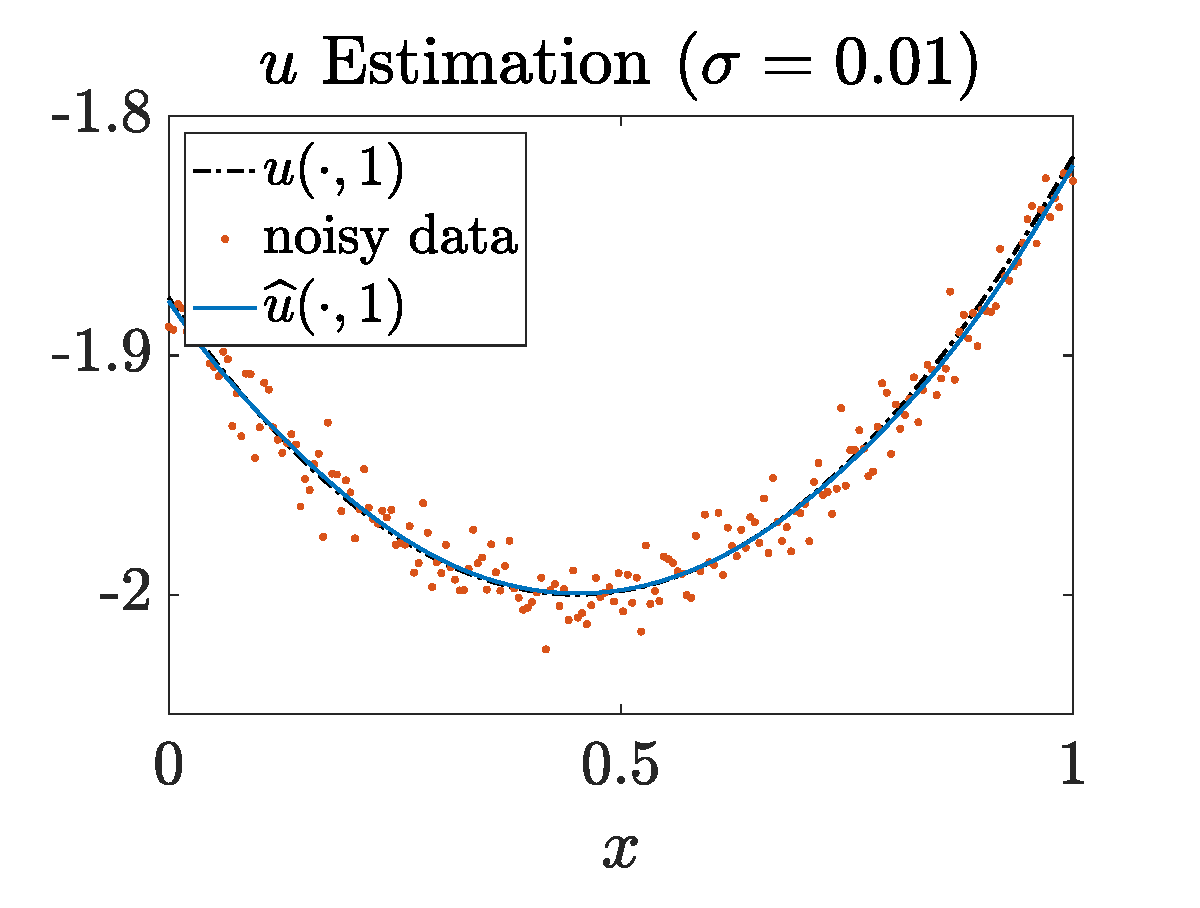
\includegraphics[width=2in]{Figures/localpolyExp1_slow.eps}&
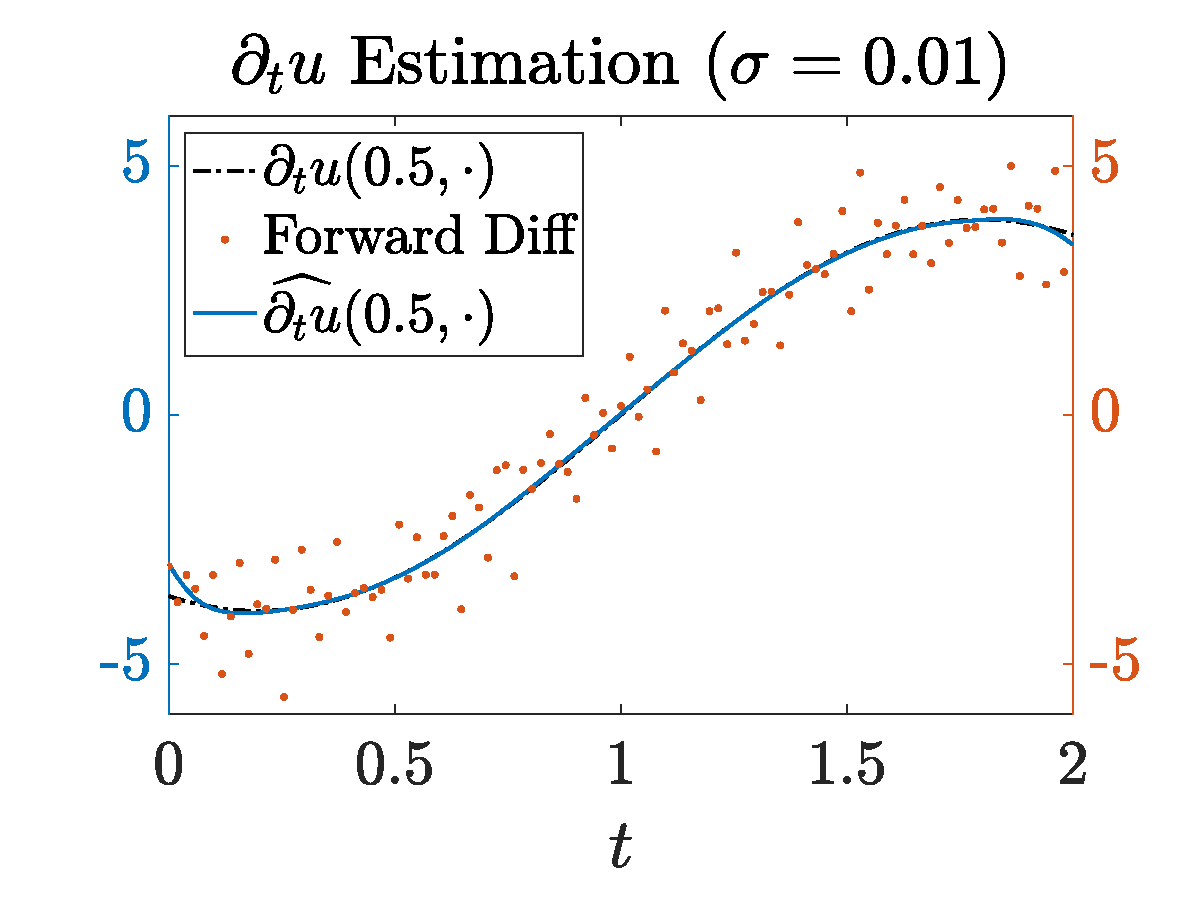
\includegraphics[width=2in]{Figures/localpolyExp3_slow.eps}&
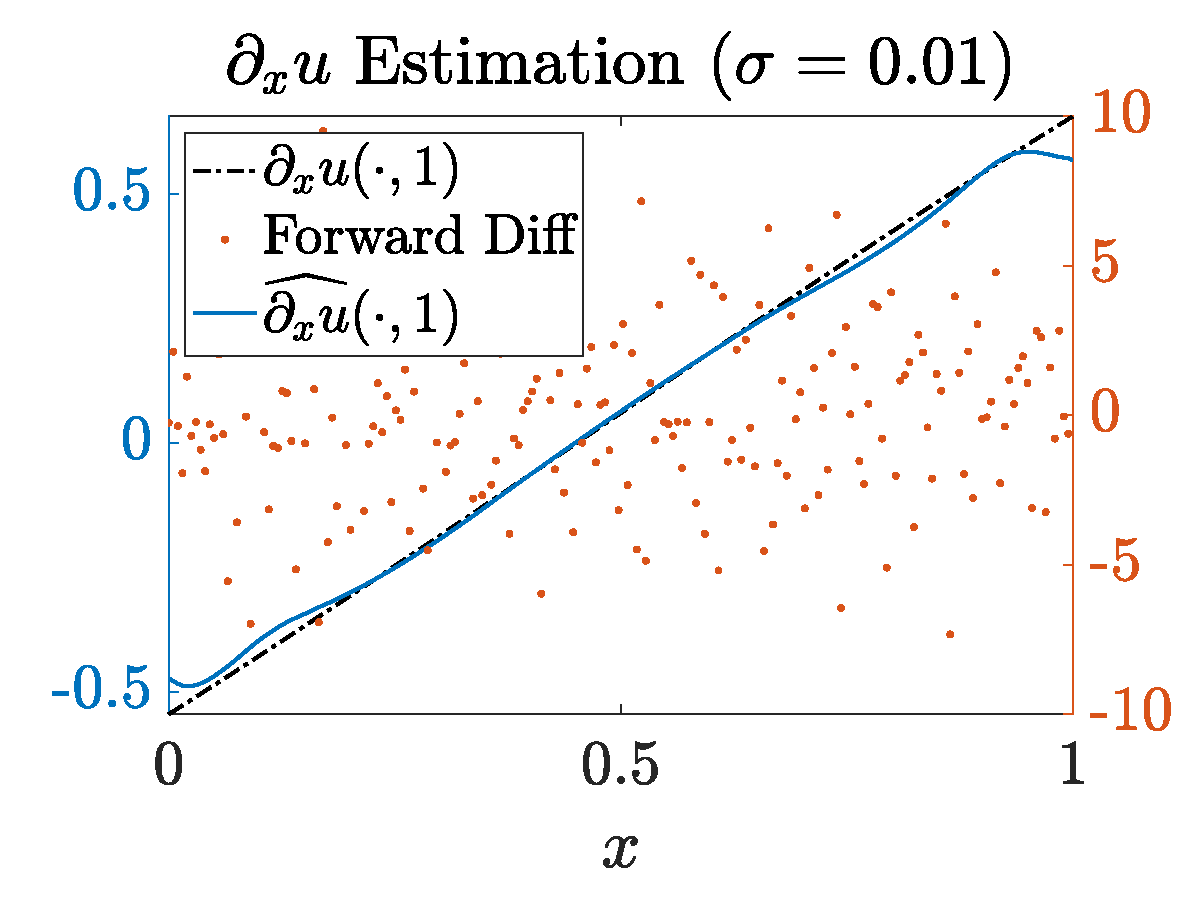
\includegraphics[width=2in]{Figures/localpolyExp2_slow.eps}
\end{tabular}
\caption{Local polynomial regression estimation for  $u(x,t) = 2\sin(\pi(x-2.5t)/4)$, for $0\leq x\leq 1$ and $0\leq t\leq 2$, and its derivatives using noisy data ($\sigma=0.01$). (a) $u$ versus $\widehat{u}$ when $t=1$. (b) $u_t$ versus $\widehat{u_t}$ when $x=0.5$ (c) $\partial_xu_x$ versus $\widehat{\partial_xu}$ when $t=1$.  $\Delta x=1/(M-1)$ and $\Delta t = 1/(N-1)$, where $M=200$ and $N=M^{7/8}\approx103$; $h_N=N^{-1/7}\approx0.5158$ and $w_M=1.2M^{-1/8}\approx0.6188$, which are determined by Theorem~\ref{thm1}.}\label{fig.derapprox}	
\end{figure}




\section{Recovery Theory for $\ell_1$-PsL based PDE Identification}
In this section, we present our main results on the $\ell_1$-PsL model for PDE identification. We focus on four aspects of the minimizer $\widehat{\bbeta}^\lambda$ of~\eqref{eq.lassoPSL}: uniqueness, proper support recovery ($\widehat{\bbeta}^\lambda\subseteq\bbeta^*$), $\ell_\infty$-norm of the coefficient error on true support ($||\widehat{\bbeta}_mS^\lambda-\bbeta_mS^*||_\infty$), and signed support recovery ($\text{sgn}\,\widehat{\bbeta}^\lambda=\text{sgn}\,\bbeta^*$). These properties strongly affect the behaviors of the identified PDE compared to those of the underlying PDE. We show that, under some assumptions, the PDE identified by the $\ell_1$-PsL model converges to the true PDE with high probability.

Here is an outline of our strategy: Using the \textit{primal-dual witness method} (PDW)~\cite{wainwright2009sharp}, we construct the pair $(\check{\bbeta},\check{\mathbf{z}})\in\mathbb{R}^{K}\times\mathbb{R}^{K}$ with $\check{\bbeta}$ satisfying the KKT equation associated with~\eqref{eq.lassoPSL} such that $\mS(\check{\bbeta})=\mS(\bbeta^*)$, and $\check{\mathbf{z}}$ being a subgradient of the $\ell_1$-norm evaluated at $\check{\bbeta}_\mS$. The desired properties of $\widehat{\bbeta}^\lambda$ hold immediately if $||\check{\mathbf{z}}||_\infty<1$ with high probability, based on Lemma 2 and 3 of~\cite{wainwright2009sharp}. It turns out that bounding the norm of the PDE estimation error  $||\btau||_\infty$ is sufficient. This quantity is further associated with two important aspects of the local polynomial regression estimation: asymptotic bias~\cite{fan1997local} and asymptotic uniform convergence~\cite{mack1982weak}. With well-designed bandwidths for the kernel of the local polynomial regression, we complete the proof. Before stating the main results, we list important assumptions in Section~\ref{sec.assumptions}.



\subsection{Model Assumptions and Implications on PDEs}\label{sec.assumptions}
We introduce three key conditions whose deterministic versions are frequently assumed to hold in $\ell_1$-regularized regression models. They were introduced during the process of proving sufficient conditions for exact sparse recovery. In our context, they carry special meanings and impose general properties on the observed solution $u$ and the underlying PDEs for a successful PDE identification from data.

\paragraph{Invertibility condition --- Identifiability of PDE from single solution}
\begin{align}
\widehat{\bF}_{\mS}^T\widehat{\bF}_\mS~\text{is invertible, almost surely.}~\label{assum1}\tag{A1}
\end{align}
This assumption is traditionally linked to the uniqueness of the solution of a linear regression model. If it fails, multicolinearity exists among the columns of $\widehat{\bF}_\mS$, which leads to intrinsic ambiguity in the modeling. The necessity of~\eqref{assum1} largely depends the fact that, in many practical settings, e.g., ocean surface monitoring~\cite{fox2001monitoring} and flock tracking~\cite{michele2016radar}, we may not be able to record multiple solutions of a single PDE determined by some unique combination of numerous known and unknown environmental factors. For example, it is impossible to choose between $u_t=3u_{xx}+u_x$ and $u_t = 5u_{xx}+u_x$ when we only observe $u(x,t)=x+t$. In Section~\ref{sec.invertibility}, we prove that, provided with sufficiently many data, \eqref{assum1} is equivalent to whether $u$ is a common solution of the underlying PDE and a derived test PDE.

\paragraph{Mutual incoherence condition --- Exhibition of signature variation} For some \textit{incoherence parameter} $\mu\in (0,1]$ and $P_\mu\in [0,1]$:
\begin{align}
\mathbb{P}\big[||\widehat{\bF}_{\mS^c}^T\widehat{\bF}_\mS(\widehat{\bF}_{\mS}^T\widehat{\bF}_\mS)^{-1}||_\infty\leq 1-\mu\big]\geq P_\mu\;.\label{assum2}\tag{A2}
\end{align}
Compared to the invertibility condition~\eqref{assum1},~\eqref{assum2} is  quantitative and more challenging to verify. This condition sets apart the group of correct feature variables from the the group of the others with probability $P_\mu$. A larger $\mu$ indicates less similarity between these two groups, thus it is easier to identify the correct model. In the literature, the deterministic version of~\eqref{assum2} is called the \textit{mutual incoherence condition}~\cite{fuchs2005recovery, tropp2006just,wainwright2009sharp}, and we refer the readers to~\cite{van2009conditions} for more well-known recoverability conditions and discussion on their relations.

The validity of \eqref{assum2} is closely related to the characteristic shapes or movements of the solution $u$. Intuitively, this means that, the observed solution $u$ of the underlying PDE needs to present the signature variation within the time-space domain for us to distinguish the correct feature variables from the others.
\paragraph{Minimal eigenvalue condition ---Threshold on noticeable magnitude} There exists some constant $C_{\min}>0$ such that:
\begin{align}
\Lambda_{\min}\Big(\frac{1}{NM}\widehat{\bF}_\mS^T\widehat{\bF}_\mS\Big)\geq C_{\min}\;,~\text{almost surely.}\label{assum3}\tag{A3}
\end{align}
Here $\Lambda_{\min}(\mathbf{A})$ denotes the minimal eigenvalue of a square matrix $\mathbf{A}\in\mathbb{R}^{n\times n}$. This condition can be considered as strengthend~\eqref{assum1}. Similarly to~\eqref{assum2},~\eqref{assum3} concerns the quantitative properties of the feature variables associated with the solution $u$. However,~\eqref{assum3} generally does not involve the characteristic variation of $u$ that is unique to the combination of the underlying feature variables.

\subsection{Main Result: Uniqueness and Proper Support Recovery}

\begin{thm}\label{thm1}
Provided with $\mathcal{D}=\{(X_i,t_n,U_i^n)~|~i=0,1,\cdots,M-1,~n=0,1,\cdots,N-1\}\subset\Omega$ and under the assumptions in Section~\ref{sec.assumptions}, there exists a constant $C'>0$ independent of $N$ and $M$, such that if we take $M = N^{(6+P_{\max})/7}$, $h_N=N^{-1/7}$ in the time direction, $w_{M} = M^{-1/(6+P_{\max})}$ in the space direction, and
\begin{align}
\lambda\geq \frac{C'}{\mu}\sqrt{\frac{K(6+P_{\max})\ln N}{7N^{4/7}}}\;,\label{lambdaBound}
\end{align}
then with probability greater than
\begin{align}
	P_\mu-\underbrace{(8K+2)N^{(13+P_{\max})/7}K\exp(-\frac{(N^{1/7}-||u||_{L^\infty(\Omega)})^2}{2\sigma^2})}_{:=P'(K,N,\sigma,||u||_{L^\infty(\Omega)})~\text{or simply}~P'}\longrightarrow P_\mu\;,~\text{as}~N\to\infty\;,\label{eq.probability}
\end{align}
the minimizer $\widehat{\bbeta}^\lambda$ of~\eqref{eq.lassoPSL} is unique, and its support is properly contained in the true support:
\begin{align}
\mS(\widehat{\bbeta}^\lambda)\subseteq\mS(\bbeta^*)\;.
\end{align}	
\end{thm}
\begin{proof}
See Appendix~\ref{app.proofthm1}	
\end{proof}


In the proof of Theorem~\ref{thm1}, we apply the PDW technique~\cite{wainwright2009sharp} to arrive at the necessary conditions for the PDW dual variable $\widetilde{\mathbf{z}}$ to be a local minimizer. Whether the support of $\widehat{\beta}^\lambda$ is contained in the true support depends on the magnitude of $||\check{\mathbf{z}}_{S^c}||_\infty$, which involves a careful estimation of the error $\btau$ defined in~\eqref{eq.tau}, which is a random vector with inaccessible probability distribution.  To overcome this difficulty, we propose to combine the results in~\cite{fan1997local} and~\cite{mack1982weak}, and derive an explicit upper-bound  for $||\btau||_\infty$ as $N,M\to\infty$ in probability. This strategy is similarly applied in~\cite{liang2008parameter} to prove the asymptotic convergence of the PsL estimators for dynamical systems. We also note that in~\cite{wainwright2009sharp}, they apply the Chernoff inequality to control  $||\check{\mathbf{z}}_{S^c}||_\infty$, under the assumption that the model residue is i.i.d.~subgaussian, which in our case does not hold in general.

The threshold for $\lambda$ characterized by~\eqref{lambdaBound} shows that when the number of data increases, there is more flexibility in tuning this parameter. If the incoherence parameter $\mu$ is small, or equivalently, the group of correct feature variables and the group of the others are similar, then the threshold~\eqref{lambdaBound} increases. In Theorem 1 of~\cite{wainwright2009sharp}, the threshold for the regularization parameter shows consistent behavior.
\begin{figure}
\centering
\begin{tabular}{ccc}
(a)&(b)&(c)\\
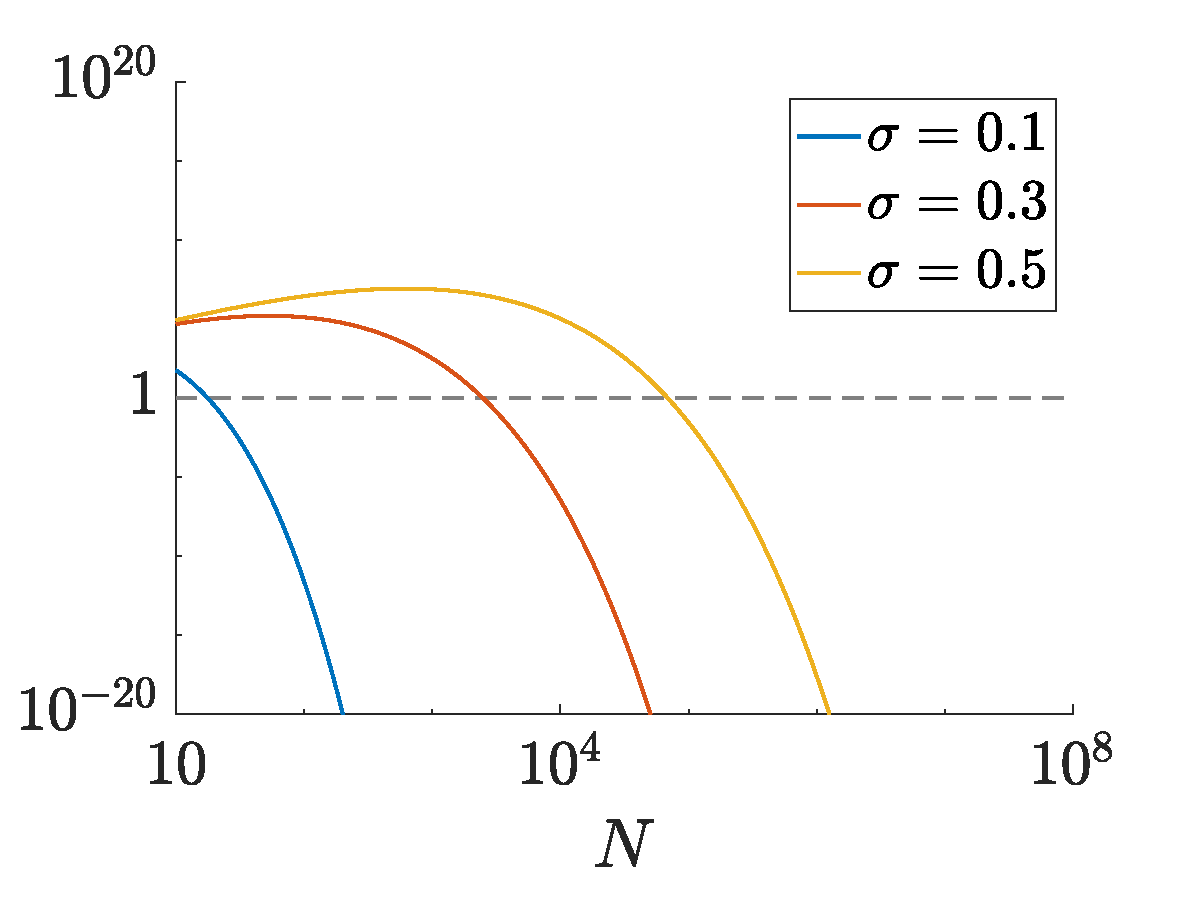
\includegraphics[width=2in]{Figures/prob1.eps}&	
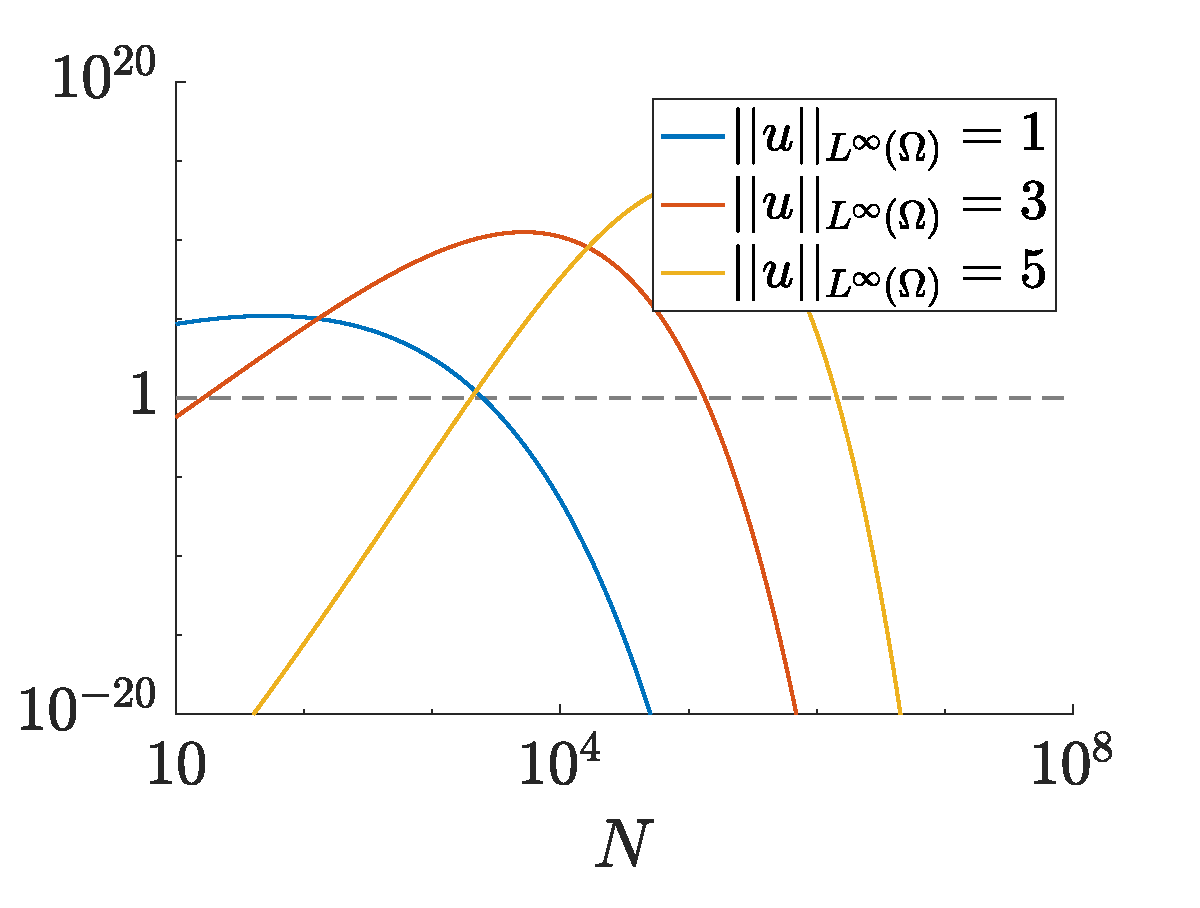
\includegraphics[width=2in]{Figures/prob2.eps}&
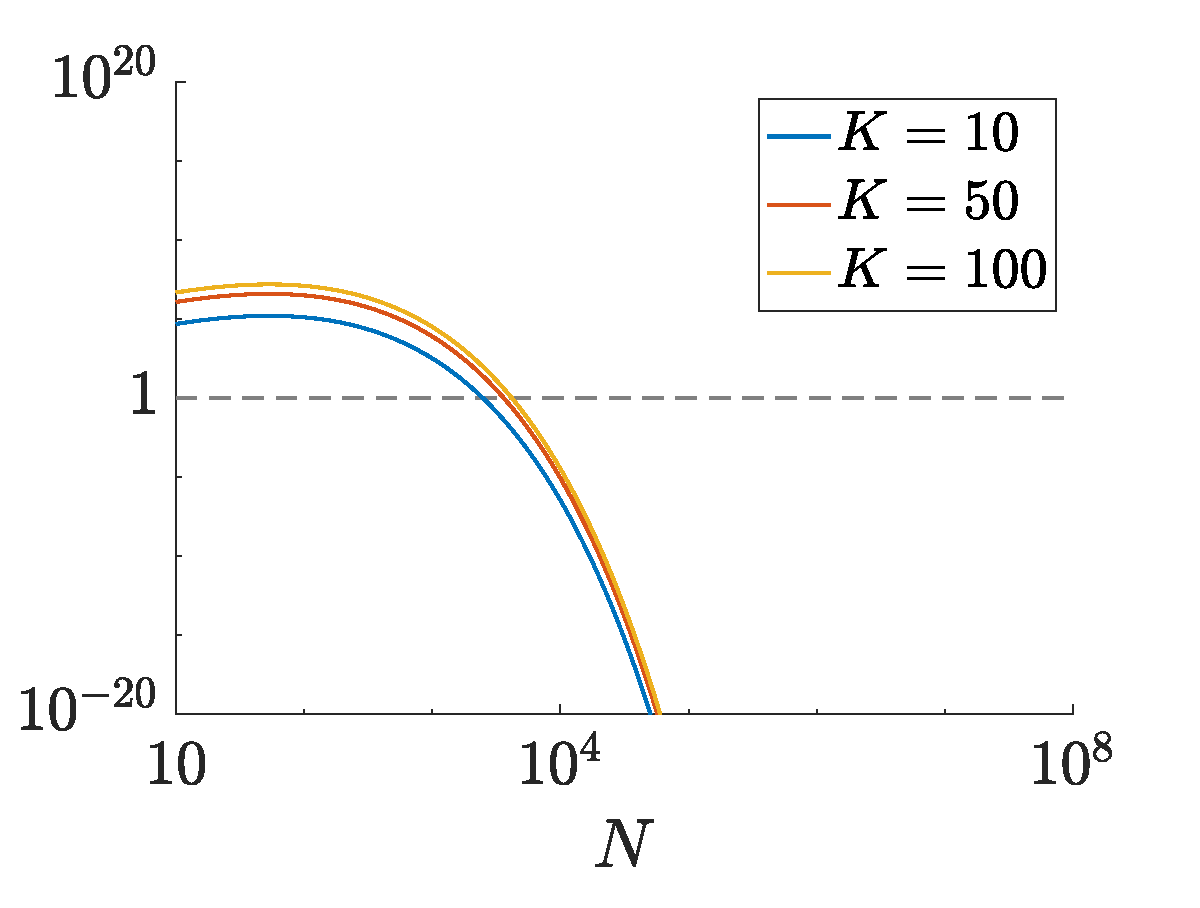
\includegraphics[width=2in]{Figures/prob3.eps}
\end{tabular}
\caption{As $N$ increases, the variation of $P'(K,N,\sigma,||u||_{L^\infty(\Omega)})$ for different (a) noise level $\sigma$ ($||u||_{L^\infty(\Omega)}=1$, $K=10$); (b) solution bound $||u||_{L^\infty(\Omega)}$ ($\sigma=0.3$, $K=10$); and (c) number of candidate feature variables $K$ ($\sigma=0.3$, $||u||_{L^\infty(\Omega)}=3$). In all cases, $P_{\max}=2$.}\label{fig.probstudy}
\end{figure}

It is worthy noticing that, $P_\mu-P'$ in~\eqref{eq.probability} is truly a probability for sufficiently large $N$, and $P'$ reduces to $0$ exponentially fast after certain amount of data is collected. Figure~\ref{fig.probstudy} shows the dependence of $P'$ on the noise level $\sigma$, solution bound $||u||_{L^\infty(\Omega)}$, and the number of candidate feature variables $K$. As seen in (a), when the underlying data is contaminated by heavier noise, it requires more data to guarantee the conclusion of Theorem~\ref{thm1} with high probability. (b) shows that with higher function magnitude, the range for $P'$ exceeding $1$ becomes narrower. There is little effect of $K$ on the effectiveness of~\eqref{eq.probability} as shown in (c).

Unlike Theorem 1 of~\cite{wainwright2009sharp}, the uniqueness and proper support recovery in our case hold only up to probability $P_\mu\in [0,1]$, rather than $1$ as $N\to\infty$. The limiting probability $P_\mu$ is determined by the mutual incoherence condition~\eqref{assum2}; therefore, for different combinations of the observe solution and the underlying PDE, the certainty about the conclusion in Theorem~\ref{thm1} can vary. We numerically study $P_\mu$ for various examples in Section~\ref{sec.numerical} which demonstrate this complexity.

We also observe that the highest partial derivative order of the candidate feature variables, $P_{\max}$, has effect on the convergence rate of~\eqref{eq.probability}. The accuracy of high-order derivative estimation is deprecated using local polynomial regression. We  often need to set $P_{\max}$ large enough to lower the model bias.  The larger $P_{\max}$ indicates more data is needed before $P'$ starts to exponentially drops to $0$.
\subsection{$\ell_\infty$ Error Bound and Signed Support Recovery}
From~\eqref{eqKKT2}, let $\Delta \bu_t=\widehat{\bu}_t-\bu_t$, $\Delta \bF=\widehat{\bF}-\bF$ denote the error terms, then we  have:
\begin{align*}
\bbeta-\bbeta^*=\Big(\widehat{\bF}^T\widehat{\bF}\Big)^{-1}	\Big[\widehat{\bF}^T(\Delta \bu_t-\Delta \bF\bbeta^*)-\lambda NM \mathbf{z}\Big]\;.
\end{align*}
Focusing on the indices corresponding to the support of $\bbeta^*$, the error of the coefficient estimation is bounded
\begin{align*}
\max_{k\in \mS}|\bbeta_k-\bbeta^*_k|&\leq	||\Big(\widehat{\bF}_S^T\widehat{\bF}_\mS\Big)^{-1}||_\infty||\widehat{\bF}_\mS^T\btau||_\infty+\lambda NM||\Big(\widehat{\bF}_\mS^T\widehat{\bF}_\mS\Big)^{-1}||_\infty\\
&\leq ||\Big(\widehat{\bF}_\mS^T\widehat{\bF}_\mS/(NM)\Big)^{-1}||_\infty\,\big(||\widehat{\bF}_\mS^T\btau||_\infty/(NM)+\lambda\big)\\
&\leq \sqrt{K}C_{\min}\,\big(||\widehat{\bF}_\mS^T\btau||_\infty/(NM)+\lambda\big)\\
&\leq \sqrt{K}C_{\min}\,\Big((||\bF_\mS||_1+||\Delta \bF_\mS||_1)\frac{||\btau||_\infty}{NM}+\lambda\Big)\\
&\leq \sqrt{K}C_{\min}\,\Big((||\bF_\mS||_1+NM\sqrt{K}||\Delta \bF||_{\max})\frac{||\btau||_\infty}{NM}+\lambda\Big)\\
&=\sqrt{K}C_{\min}\,\Big(\frac{||\bF_\mS||_1||\btau||_\infty}{NM}+\sqrt{K}||\Delta \bF||_{\max}||\btau||_\infty+\lambda\Big)
\end{align*}
Hence, applying Theorem~\ref{theorem.main1} and Lemma 3 (b) of~\cite{wainwright2009sharp} gives the following result.
\begin{thm}\label{inftythm}
Suppose the conditions for Theorem~\ref{thm1} hold,  with probability greater than
\begin{align}
	P_\mu-(8K+2)N^{(13+P_{\max})/7}K\exp(-\frac{(N^{1/7}-||u||_{L^\infty(\Omega)})^2}{2\sigma^2})\longrightarrow P_\mu\;,~\text{as}~N\to\infty\;,
\end{align}
then
\begin{align}
||\widehat{\bbeta}_\mS^\lambda-\bbeta_\mS^*||_\infty\leq \sqrt{K}C_{\min}\,\Big(\frac{C'\big(||\bF_\mS||_1+C'\sqrt{K}\big)}{N^{(19+P_{\max})/7}}+\lambda\Big)\;.\label{infbound}
\end{align}
Moreover, if $\min_{k\in \mS}|\bbeta_k^*|>\sqrt{K}C_{\min}\,\Big(\frac{C'(||\bF_\mS||_1+C'\sqrt{K})}{N^{(19+P_{\max})/7}}+\lambda\Big)$, then $\widehat{\bbeta}^\lambda$ has the correct signed support.
\end{thm}
The upper-bound for the $\ell_\infty$-norm of the coefficient error in~\eqref{infbound} consists of two components. The first one contains information about the underlying PDE, the data size, and the number of candidate features. As $N$ increases to $\infty$, this part converges to $0$ without explicit dependence on the choice of feature variables selected from $\ell_1$-PsL. The second component is simple: $\sqrt{K}C_{\min}\lambda$. When $N$ increases, this part does not vary. However, we note that by adjusting $\lambda$ so that it is above the threshold stated in Theorem~\ref{thm1}, $\ell_1$-PsL is guaranteed to recover the correct feature variables under some conditions. Since the threshold~\eqref{lambdaBound} decreases to $0$ as $N\to\infty$, we see that we can choose smaller $\lambda$ to achieve the recovery. As an overall effect,  increasing the data size $N$ leads to more accurate coefficient estimation.

An important implication of Theorem~\ref{inftythm} is the correct signed support. Many PDEs are sensitive to the sign of the coefficients. For example, changing the sign of the advection term in transport equation reverses the moving direction, and changing the sign of the laplacian term of the heat equation leads to instability.  Theorem~\ref{inftythm} guarantees the correct signs provided that the magnitudes of the coefficients of the correct feature variables are larger than a threshold same as~\ref{infbound}. Therefore, asymptotically, we are sure that the recovered coefficients are close to the true ones and that the signs are correct, even for those with small absolute values.
\section{Recoverability Conditions and PDE Identification}
\subsection{Invertibility Condition}\label{sec.invertibility}
When there exist sufficiently many data, we prove that \eqref{assum1} fails if and only if the observed function $u$ is a common solution of the underlying PDE and a derived test PDE. The  test PDE is a stationary ($u_t=0$) PDE of the same type as the underlying one, i.e., the coefficient vectors for the feature variables share the same support. First, we prove the following technical lemma:
\begin{lemma}\label{nonoise_lemma}
Denoting $\bF_p$ as the column of the feature matrix corresponding to the feature $\partial_x^p u$, $p=0,1,\cdots,P_{\max}$, then
\begin{align}
	\abs{\int_\Omega \partial_x^pu(x,t)\,dx\,dt-\mathbf{1}^T\bF_p\Delta x\Delta t}\to 0\;,
\end{align}
as the resolution $\Delta x,\Delta t\to 0$. Here $\mathbf{1}\in\mathbb{R}^{NM}$ is the $1$-vector. Similarly, if $\bF_{p,q}$ denotes the column of the feature matrix corresponding to the product feature $\partial_x^pu\,\partial_x^qu$, then
\begin{align}
	\abs{\int_\Omega\partial_x^pu(x,t)\partial_x^qu(x,t)\,dx\,dt-\bF_{p}^T\bF_{q}\Delta x\Delta t}\to 0\;.
\end{align}
\end{lemma}
\begin{proof}
See Appendix~\ref{proof_nonoise_lemma}.	
\end{proof}

Lemma~\ref{nonoise_lemma} justifies using the normal matrix $\bF^T\bF\Delta x\Delta t$ to approximate the Gram matrix $\mathbf{G}$ whose $(j,k)$-entry is the $L^2(\Omega)$ inner product of the $j$-th and $k$-th  candidatefeature variable, when there are sufficiently many data. Since it is well-known that the Gram matrix is invertible if and only if its associated vectors are linearly independent, we have the following characterization:
\begin{prop}\label{prop.invert}Suppose an evolutionary function $u:\Omega\to\mathbb{R}$, i.e., $u_t\neq 0$, satisfies~\eqref{eq.PDE2}. When the number of data is sufficiently large,  $\bF_\mS^T\bF_\mS$ is not invertible if and only if $u$  also satisfies a stationary PDE:
\begin{align}
&0= F(u,u_x,u_{xx}\dots;\widetilde{\bbeta}):=\widetilde{\beta}_0+\widetilde{\beta}_1u+\widetilde{\beta}_2u_x+\widetilde{\beta}u_{xx}+\dots+\widetilde{\beta}_{p,q}\partial^p_xu\partial^q_xu+\dots	\;,\nonumber\\
&(x,t)~\text{in}~\Omega = (0,X_{\max})\times(0,T_{\max})\;,\label{eq.PDEtest}
\end{align}
for some  $\widetilde{\bbeta}\in\mathbb{R}^{K}$ which has the same support as $\bbeta^*$.
\end{prop}

In this paper, we call the stationary PDE~\eqref{eq.PDEtest} as the \textit{test PDE} associated with the solution-PDE pair $\big(u,\mathcal{F}(\cdot,\bbeta^*)\big)$. Notice that the test PDE is essentially an ordinary differential equation (ODE); hence, verifying~\eqref{assum1} involves solving  the test PDE then plugging it to the original.

For any PDEs consisting of one feature variable, i.e., $\abs{\mS(\bbeta^*)}=1$, with sufficiently many data, the invertibility condition~\eqref{assum1} always holds for any non-stationary function $u$, $u_t\neq 0$. This includes non-stationary solutions of transport equation, heat equation, or inviscid Burgers equation, etc. In the following, we show some non-trivial examples.
\begin{figure}
\centering
\begin{tabular}{ccc}
(a)&(b)&(c)\\
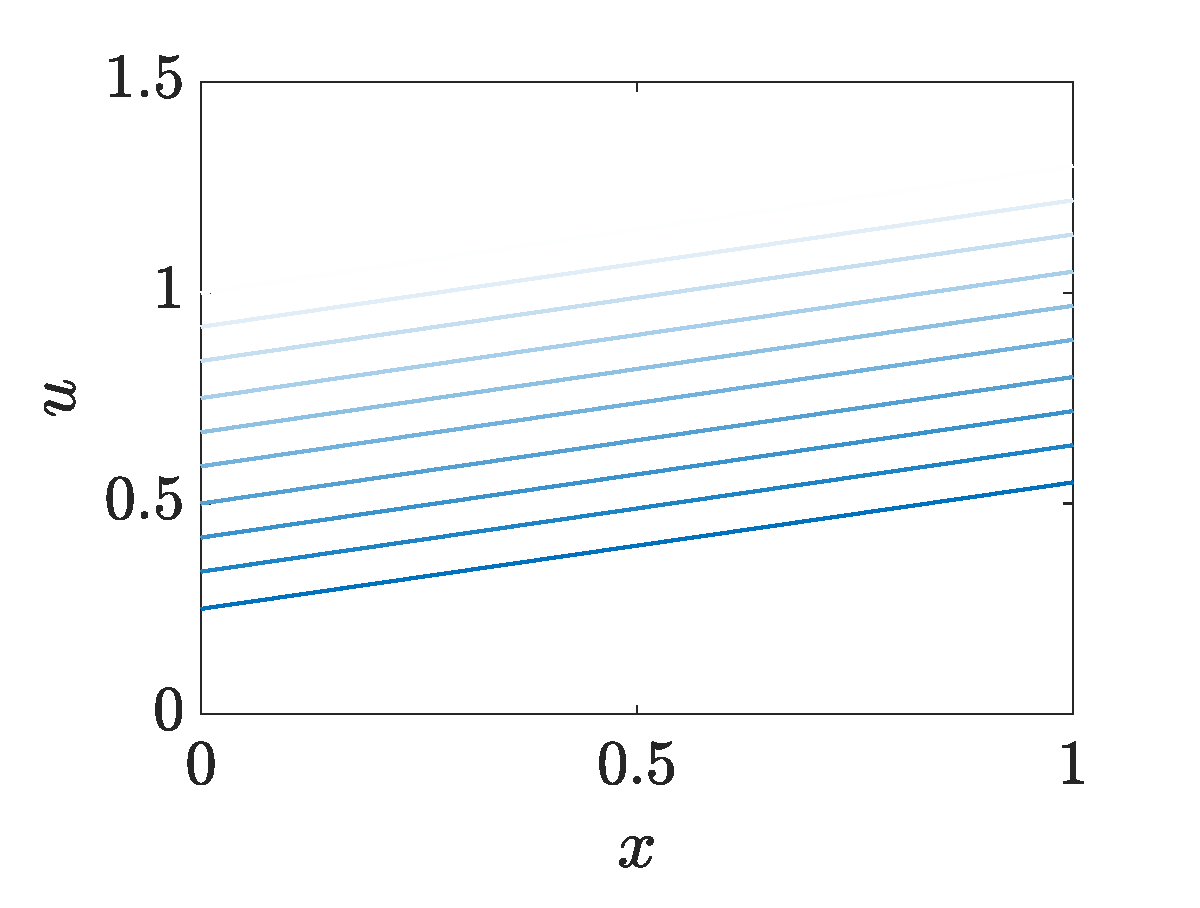
\includegraphics[width=2in]{Figures/advdiffExp2.eps}&
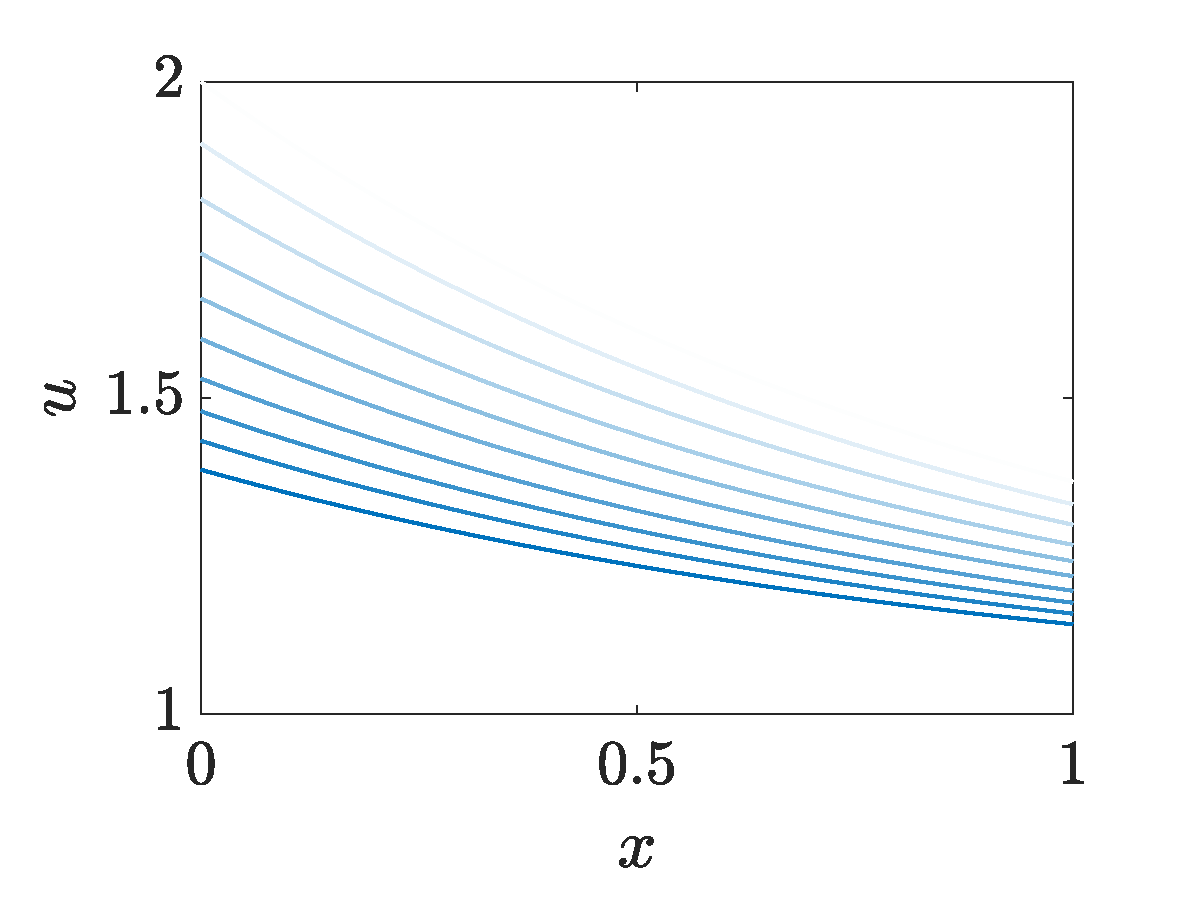
\includegraphics[width=2in]{Figures/advdiffexp1.eps}&
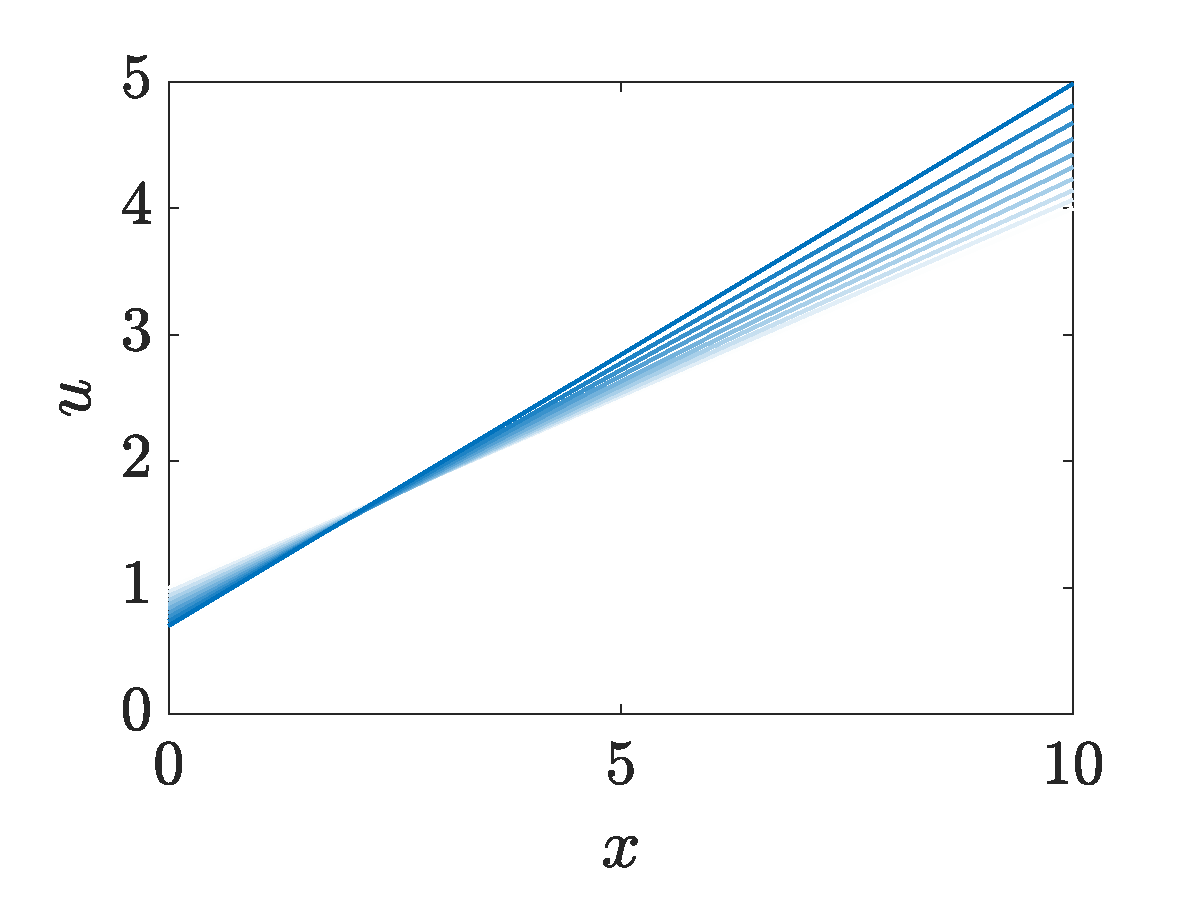
\includegraphics[width=2in]{Figures/vBurgersExp1.eps}
\end{tabular}
\caption{Special solutions that fail~\eqref{assum1}. (a) A solution for the advection-diffusion equation~\eqref{advdiff}. (b) Another solution for the advection-diffusion equation~\eqref{advdiff}. (c) A solution for the viscous Burgers' equation~\eqref{original.Burger}. Curves with lighter color represents the solution at earlier time.}\label{fig.invertibility}	
\end{figure}

\begin{example}
Consider an advection-diffusion equation:
\begin{align}
&u_t=Du_{xx}-vu_x\;,~0<x<X_{\max},0<t<T_{\max}\;,\label{advdiff}
\end{align}
where $D>0$ is the diffusitivity coefficient, and $v>0$ is the advection speed. It describes the evolution of the concentration distribution of a non-decaying pollutant in a flowing stream. Suppose we observe a solution $u$ of \eqref{advdiff} which also satisfies the test PDE:
\begin{align}
au_{xx}+bu_{x}=0\label{eq.test}	
\end{align}
for some $a,b\in\mathbb{R}$ such that $a^2+b^2\neq 0$.
\begin{enumerate}
\item If $b= 0$, then solving~\eqref{eq.test} gives $u=A(t)x+B(t)$ for arbitrary functions $A$ and $B$; plugging this into PDE~\eqref{advdiff} leads to:
\begin{align}
\begin{cases}
A(t)=A_0\\
B(t) = -vA_0t+B_0\;
\end{cases}\,,\quad 0\leq t\leq T_{\max}
\end{align}
where $A_0$ and $B_0$ are arbitrary constants.
\item If $a=0$,~\eqref{eq.test} gives $u=A(t)$ for an arbitrary function $A$; plugging this into~\eqref{advdiff} leads to  that $u$ is stationary, hence a contradiction.
\item If $a\neq0$ and $b\neq 0$,  solving~\eqref{eq.test} gives $u=A(t)+B(t)\exp(-bx/a)$; then~\eqref{advdiff} implies:
\begin{align}
\begin{cases}
A(t)=A_0\\
B(t)=B_0\exp\big((Db^2/a^2+vb/a)t\big)
\end{cases}\,,\quad 0\leq t\leq T_{\max}\label{test3}	
\end{align}
\end{enumerate}
To sum up, with sufficiently many data, if we observe $u(x,t)=A_0x-vA_0t+B_0$ or $u(x,t)=A_0+B_0\exp((Db^2/a^2+vb/a)t-bx/a)$ for arbitrary constants $A_0,B_0$, $A_0^2+B_0^2\neq 0$, then the invertibility condition~\eqref{assum1} associated with the PDE~\eqref{advdiff} fails. In Figure~\ref{fig.invertibility}, we show the special solution $u(x,t)=0.3x-0.75t+1$ in (a) and $u(x,t)=1+\exp(-0.95t-x)$ in (b) for illustration.
\end{example}
\begin{example}
Consider the viscous Burgers' equation:
\begin{align}
u_t=Du_{xx}+uu_x\label{original.Burger}	
\end{align}
which is the fundamental model for the dissipative system such as traffic flow. The associated test PDE is the following
\begin{align}
au_{xx}+buu_{x}=0\label{test.Burger}	
\end{align}
with $a^2+b^2\neq 0$.
\begin{enumerate}
\item If $a = 0$, then~\eqref{test.Burger} leads to a general solution $u=A(t)$ for an arbitrary function $A$. However,~\eqref{original.Burger} then forces that $u$ to be a constant; hence, $a\neq 0$.
\item If $b = 0$, then~\eqref{test.Burger} leads to a general solution $u=A(t)x+B(t)$ for  arbitrary functions $A$  and $B$.~\eqref{original.Burger} then imposes conditions:
\begin{align}
\begin{cases}
A^2(t)=A'(t)\\
A(t)B(t)-B'(t)=0
\end{cases}	\implies\begin{cases}
A(t)=\frac{A_0}{1-A_0t}\\
B(t)=1-A_0t
\end{cases}
\end{align}
where $A_0\neq 0$ is an arbitrary constant. Since we assume that $u$ is continuous in $\Omega$, $A_0<1/T_{\max}$.
\item If $a\neq 0$ and $b\neq 0$,~\eqref{test.Burger} can be transformed to a Riccati equation in terms of $u_x$, from which we may solve for the general solution of~\eqref{test.Burger} as:
\begin{align}
u(x,t)=	\frac{cA(t)\exp(\frac{bc}{a}x)-cB(t)\exp(-\frac{bc}{a}x)}{A(t)\exp(\frac{bc}{a}x)+B(t)\exp(-\frac{bc}{a}x)}\label{testsol2.Burger}
\end{align}
where $c$ is an arbitrary constant, and $A$, $B$ are arbitrary functions. By plugging~\eqref{testsol2.Burger} into~\eqref{original.Burger}, we immediately see that the common solution exists if and only if $a=2Db$, which is:
\begin{align}
u(x,t) = \frac{cA_0\exp(cx/(2D))-cB_0\exp(-cx/(2D))}{A_0\exp(cx/(2D))+B_0\exp(-cx/(2D))}\;.	
\end{align}
However, this is a stationary solution, hence a contradiction.
\end{enumerate}
In Figure~\ref{fig.invertibility} (c), we show the solution $u(x,t)=0.3x/(1-0.3t)+1-0.3t$ for illustration.
\end{example}

It is relatively easy to investigate the invertibility condition when the underlying PDE is linear. As for general nonlinear PDEs, various techniques are designed for nonlinear ODEs which can be applied to the test PDEs. In some cases, such as Fischer's equation, Korteweg-de Vries equation, etc., the solutions to the test PDEs may involve elliptic integrals, which makes it more difficult to validate the invertibility condition.

Combining Lemma~\ref{nonoise_lemma} with Corollary~\ref{cor.singlespace} and Corollary~\ref{cor.doublespace} allows us to extend the discussion above to the case where noise is included.
\begin{corollary}
Denoting $\widehat{\bF}_k$ as the column of the approximated feature matrix corresponding to the feature $\partial_x^k u$, $k=0,1,\cdots,P_{\max}$, then
\begin{align}
	\abs{\int_\Omega\partial_x^ku(x,t)\,dx\,dt-\mathbf{1}^T\widehat{\bF}_k\Delta x\Delta t}\to |\Omega|\,||\widehat{\bF}_k-\bF_k||_\infty
\end{align}
as the number of data $N,M\to\infty$. Similarly, if $\widehat{\bF}_{k,j}$ denotes the column of the feature matrix corresponding to the product feature $\partial_x^ku\,\partial_x^ju$, then
\begin{align}
	\abs{\int_\Omega\partial_x^ku(x,t)\partial_x^ju(x,t)\,dx\,dt-\widehat{\bF}_{k}^T\widehat{\bF}_{j}\Delta x\Delta t}\to |\Omega|\,||\widehat{\bF}^T_{k}\widehat{\bF}_{j}-\bF^T_{k}\bF_{j}||_\infty\;.
\end{align}

\end{corollary}
\begin{proof} By triangle inequality
\begin{align*}
	\abs{\int_\Omega \partial_x^ku(x,t)\,dx\,dt-\mathbf{1}^T\widehat{\bF}_k\Delta x\Delta t}&\leq \abs{\int_\Omega\partial_x^ku(x,t)\,dx\,dt-\mathbf{1}^T\bF_k\Delta x\Delta t}+||\widehat{\bF}_k-\bF_k||_1\Delta x\Delta t\\
	&\leq o(\Delta x) + o(\Delta t)+|\Omega|\,||\widehat{\bF}_k-\bF_k||_\infty\;.
\end{align*}
\end{proof}
\begin{corollary}
For any $\varepsilon >C'|\Omega|M^{-2/(6+p)}$ with sufficiently large $M$ and $N$, we have:
\begin{align}
\mathbb{P}\Big[\abs{\int_\Omega\partial_x^pu(x,t)\,dx\,dt-\mathbf{1}^T\widehat{\bF}_p\Delta x\Delta t}>\varepsilon\Big]<2M\exp(-\frac{M^{1/(6+p)}-||u||_{L^\infty(\Omega)}^2}{2\sigma^2})\;,
\end{align}
and
\begin{align}
\mathbb{P}\Big[\abs{\int_\Omega\partial_x^pu(x,t)\partial_x^qu(x,t)|\,dx\,dt-\widehat{\bF}^T_p\widehat{\bF}_q\Delta x\Delta t}>\varepsilon\Big]<8M\exp(-\frac{M^{1/(6+\max\{p,q\})}-||u||_{L^\infty(\Omega)}^2}{2\sigma^2})\;.
\end{align}
\end{corollary}

\subsection{Mutual Incoherence Condition}\label{sec.MIP}
Mutual incoherence condition is more challenging to verify. Intuitively, this assumption is closely related to whether the observed solution $u$ displays characteristic  movements that are representative to the underlying PDE. Therefore, the data-size, the observed solution of the underlying PDE, and the choice of candidate feature variables have deterministic impacts.
\begin{example} Diffusion and decaying can cause confusion for PDE identification. As analyzed in the previous subsection, when there is no noise, we may consider the following continuous approximation of~\eqref{assum2} provided that the candidates only include $u$ and $u_{xx}$ and $u_{xx}$ is the only true feature:
\begin{align}
\frac{|\langle u,u_{xx}\rangle_{L^2(\Omega)}|}{||u_{xx}||_{L^2(\Omega)}^2}\leq 1-\mu.\label{diffdecay}
\end{align}
Suppose the observed solution can be expressed as $u(x,t)=A(t)\cos \omega x+B(t)\sin \omega x$ for some $\omega>0$, then the quantity on the left hand side of~\eqref{diffdecay} is simply $1/\omega^2$. Therefore, when $\omega< 1$,~\eqref{diffdecay} fails; and if $\omega> 1$, it holds for some $\mu$. Due to possibly insufficient sampling, the frequency demonstrated in the data can be lowered, thus~\eqref{diffdecay} may not hold even if $\omega$ is large. We may extend the discussion here to $u$ which is analytic along space for every time, and conclude that if the observed solution consists of low frequency components in space, then~\eqref{assum2} fails when $u$ and $u_{xx}$ are the candidates. Furthermore, we mention that the statements above is exactly reversed if $u$ is the true feature instead of $u_{xx}$.
\end{example}
In Section~\ref{sec.numerical}, we look into the \textit{plane wave solutions} of a transport equation which are completely characterized by their magnitudes and wavenumbers.

\subsection{Minimal Eigenvalue Condition}\label{sec.minimalEigen}
Minimal eigenvalue condition~\eqref{assum3} is associated with the detectable magnitude of the observed solution of the underlying PDE, rather than specific features determined by the PDE. For instance, if the underlying PDE consists of only one feature variable, such as the cases in transport equation and heat equation, then~\eqref{assum3} is simply requiring that, with sufficiently many data, the $L^2(\Omega)$-norm of the  feature variable exceeds $C_{\min}>0$. We present another example to illustrate this idea.
\begin{example} If the underlying PDE is advection-diffusion equation, then the associated normal matrix $\bF_\mS^T\bF_\mS$ is:
\begin{align}
\begin{bmatrix}
||u_x||^2_{L^2(\Omega)}&\langle u_x,u_{xx}\rangle_{L^2(\Omega)}\\
\langle u_x,u_{xx}\rangle_{L^2(\Omega)}&||u_{xx}||^2_{L^2(\Omega)}
\end{bmatrix}
\end{align}
whose minimal eigenvalue $\Lambda_{\min}$ can be proved to satisfy:
\begin{align}
&0\leq \Lambda_{\min}\leq \min\{||u_x||^2_{L^2(\Omega)},||u_{xx}||^2_{L^2(\Omega)}\}\;,\quad\text{If}~\langle u_x,u_{xx}\rangle_{L^2(\Omega)}\geq 0\;;\\
&\min\{||u_x||^2_{L^2(\Omega)},||u_{xx}||^2_{L^2(\Omega)}\}\leq \Lambda_{\min}\;,\quad\text{If}~\langle u_x,u_{xx}\rangle_{L^2(\Omega)}\leq 0\;.
\end{align}
In both cases,~\eqref{assum3} holds more easily if the magnitudes of the underlying feature variables are large. An interesting aspect of this example is that, when $u_x$ and $u_{xx}$ are negatively correlated,~\eqref{assum3} immediately holds by setting $C_{\min} = \min\{||u_x||^2_{L^2(\Omega)},||u_{xx}||^2_{L^2(\Omega)}\}$.
%\begin{align}
%\lambda^2-\lambda(||u_x||_{L^2(\Omega)}+||u_{xx}||_{L^2(\Omega)})-\langle u_x,u_{xx}\rangle_{L^2(\Omega)}^2+||u_x||_{L^2(\Omega)}||u_{xx}||_{L^2(\Omega)}=0
%\end{align}
%\begin{align}
%&\frac{(||u_x||_{L^2(\Omega)}+||u_{xx}||_{L^2(\Omega)})-\sqrt{(||u_x||_{L^2(\Omega)}-||u_{xx}||_{L^2(\Omega)})^2+4\langle u_x,u_{xx}\rangle_{L^2(\Omega)}}}{2}
%\end{align}
%\begin{align}
%&\frac{(||u_x||_{L^2(\Omega)}+||u_{xx}||_{L^2(\Omega)})-\sqrt{(||u_x||_{L^2(\Omega)}-||u_{xx}||_{L^2(\Omega)})^2+4\langle u_x,u_{xx}\rangle_{L^2(\Omega)}}}{2}\leq \\
%&	\frac{(||u_x||_{L^2(\Omega)}+||u_{xx}||_{L^2(\Omega)})-\abs{||u_x||_{L^2(\Omega)}-||u_{xx}||_{L^2(\Omega)}}}{2}=\min\{||u_x||_{L^2(\Omega)},||u_{xx}||_{L^2(\Omega)}\}
%\end{align}
\end{example}



\section{Numerical Experiments}\label{sec.numerical}

\subsection{Identification of PDEs using $\ell_1$-PsL: Examples}
In this section, we apply the proposed $\ell_1$-PsL method to identify some classical PDEs using noisy data. From the huge families of PDEs, we select the heat equation (second-order linear equation) and Burgers' equation (first-order non-linear equation) as our examples here. Each of them plays a fundamental role in modeling physical phenomenon and demonstrates characteristic behaviors shared by more complex systems, such as dissipation and shock-formation. We refer the readers to~\cite{haberman1983elementary} for derivations and more.
\subsubsection{Heat Equation}
Heat equation is one of the most fundamental PDEs in physics as well as mathematics. It models the variation of the temperature distribution along a conductive material as the time proceeds. For a metal ring, one can equip the heat equation with a periodic boundary condition:
\begin{align}
&u_t(x,t) = \nu u_{xx}(x,t)\;,0<x<1,~0<t<T_{\max}\;.\label{eq.heatPDE}\\
&u(x,0)=f(x)\;, 0\leq x\leq 1\;;\label{eq.heatPDE.ival}\\
&u(0,t)=u(1,t)\;,0\leq t\leq T_{\max}\label{eq.heatPDE.bd}\;.
\end{align}
Here $u(x,t)$ denotes the temperature of the bar at location $0\leq x\leq 1 $ and time $0\leq t\leq 1$, $\nu>0$ is the material conductivity, and $f(x)$ describes the initial heat distribution on the ring.

The analytical solution of \eqref{eq.heatPDE}--\eqref{eq.heatPDE.bd} can be found via methods such as Fourier transform, and the accessibility of these formulae heavily depends on properties of $f$. Instead, we numerically solve \eqref{eq.heatPDE}--\eqref{eq.heatPDE.bd} by some finite difference scheme on a grid finer than the grid where the data $\mathcal{D}$ is located. Then, we downsample the numerical solution and add Gaussian noise to obtain $\mathcal{D}$.

Figure~\ref{fig.heat}~(a) shows the numerical solution when the initial condition is $f(x)=5(1-x)^2x\cos(3\pi x),~0\leq x\leq 1$, terminal time is $T_{\max}=0.1$, and the conductivity constant is $\nu =0.1$.  Here we solve \eqref{eq.heatPDE}--\eqref{eq.heatPDE.bd} by the FTCS scheme using $\Delta t=6.6667\times10^{-7} (=0.0033/5000)$ and $\Delta x= 0.02$, then we downsample the solution by $5000$ in time, resulting in $N=30$ and $M=50$. (b) demonstrates the noisy data ($\sigma=0.1$), from which, we apply the $\ell_1$-PsL and identify the correct PDE which reproduce the underlying dynamic in (c).

Figure~\ref{expr.heat} illustrates the dependence of the feature variable identification on the choice of $\lambda$, under different levels of noise: (a) $\sigma=0.01$, (b) $\sigma=0.1$, and (c) $\sigma=0.3$. The dashed curves represent  the coefficients of the false features, and the red one represents that of the correct one.  As $\lambda$ increases, the false feature variables are filtered out, while the correct one $u_{xx}$ remains active. As the noise level increases, it becomes more difficult to separate the correct feature variables from the false: The vanishing points of the dashed curves are approaching to that of the red curve.
\begin{figure}
\centering
\begin{tabular}{ccc}
(a)&(b)&(c)\\
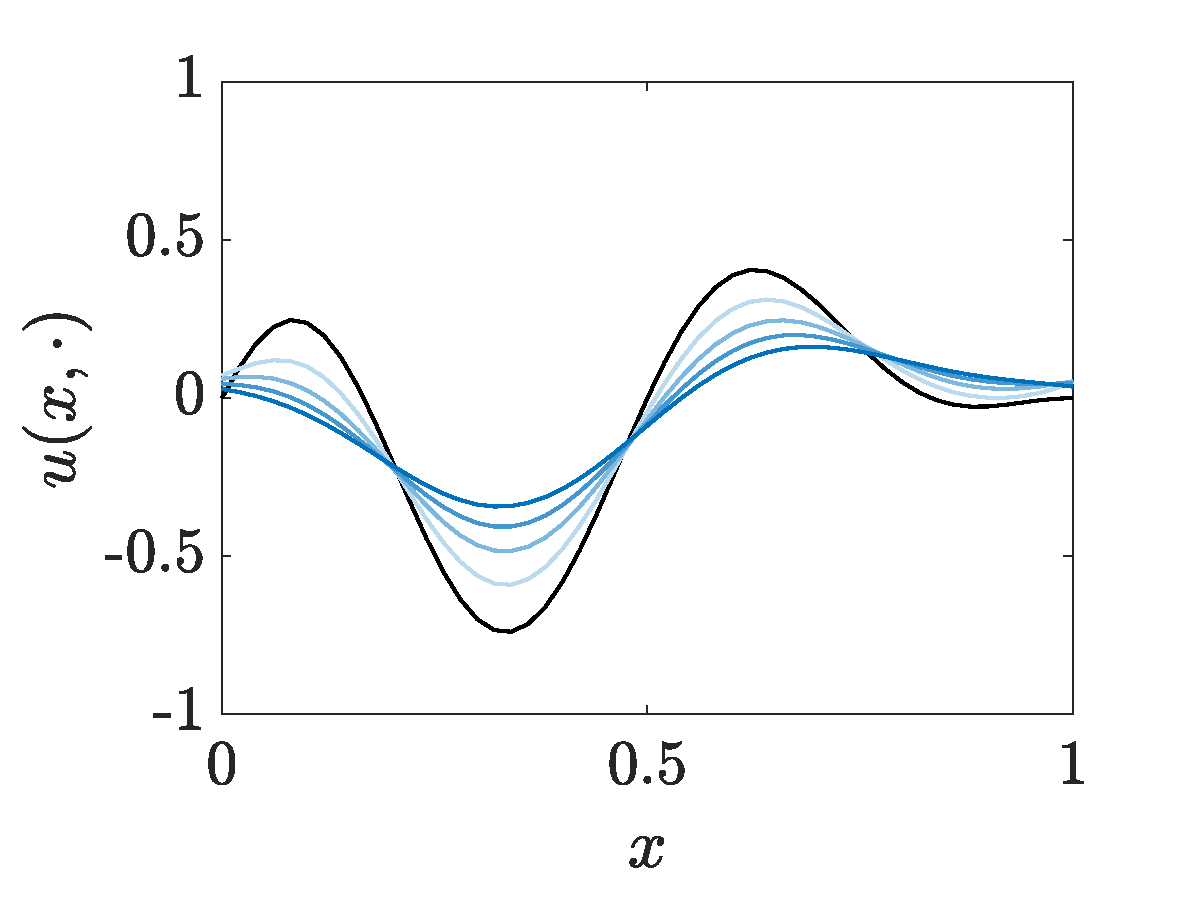
\includegraphics[width=2in]{Figures/heat_sol.eps}&
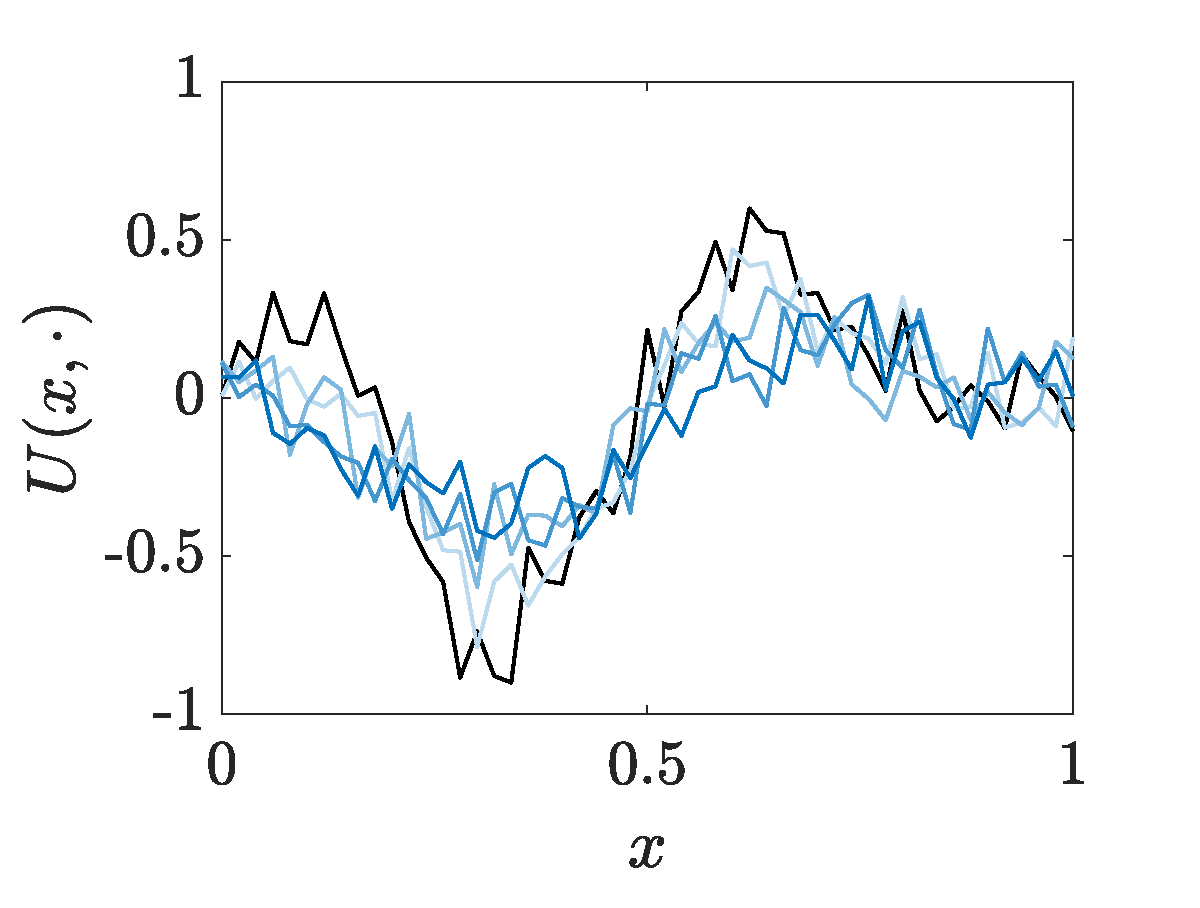
\includegraphics[width=2in]{Figures/heat_noise.eps}&
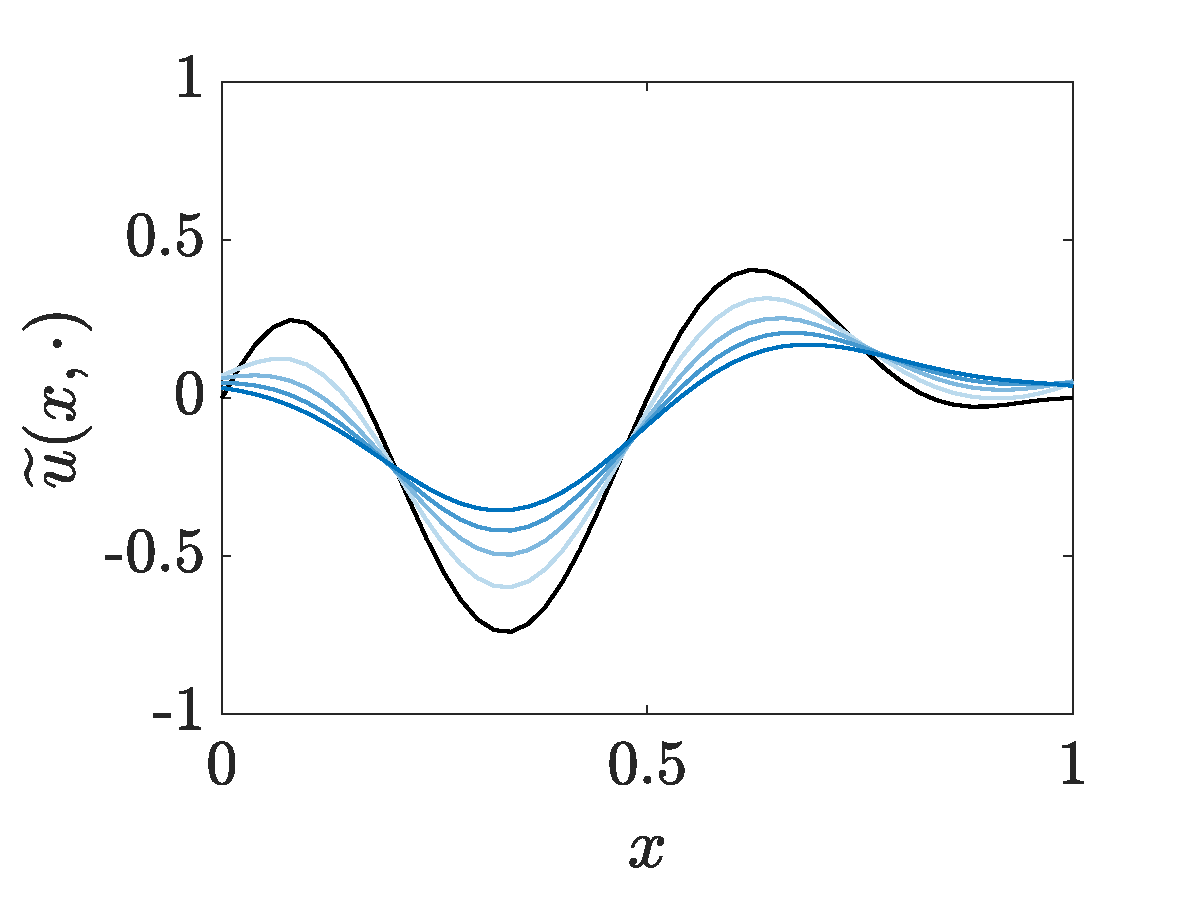
\includegraphics[width=2in]{Figures/heat_resimu.eps}
\end{tabular}
\caption{[Heat equation] (a) Numerical solution of $u_t=0.1u_{xx}$ with initial condition: $f(x)=5(1-x)^2x\cos(3\pi x),~0\leq x\leq 1$. (b) Data obtained from (a) with additive Gaussian noise of intensity $\sigma=0.1$. (c) Numerical solution of the identified PDE: $u_t=0.0939u_{xx}$. }	\label{fig.heat}
\end{figure}
\begin{figure}
\centering
\begin{tabular}{ccc}
(a)&(b)&(c)\\
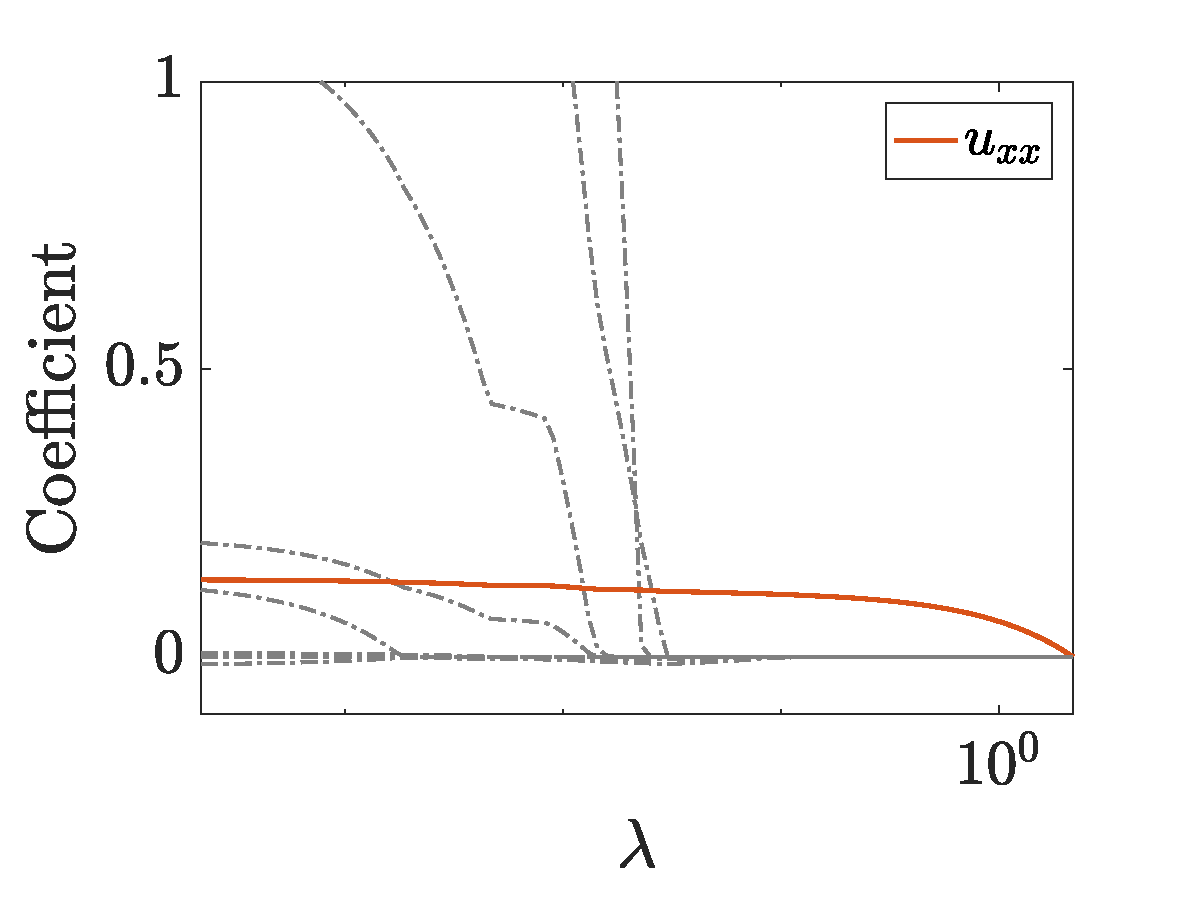
\includegraphics[width=2in]{Figures/heat_0_01.eps}&
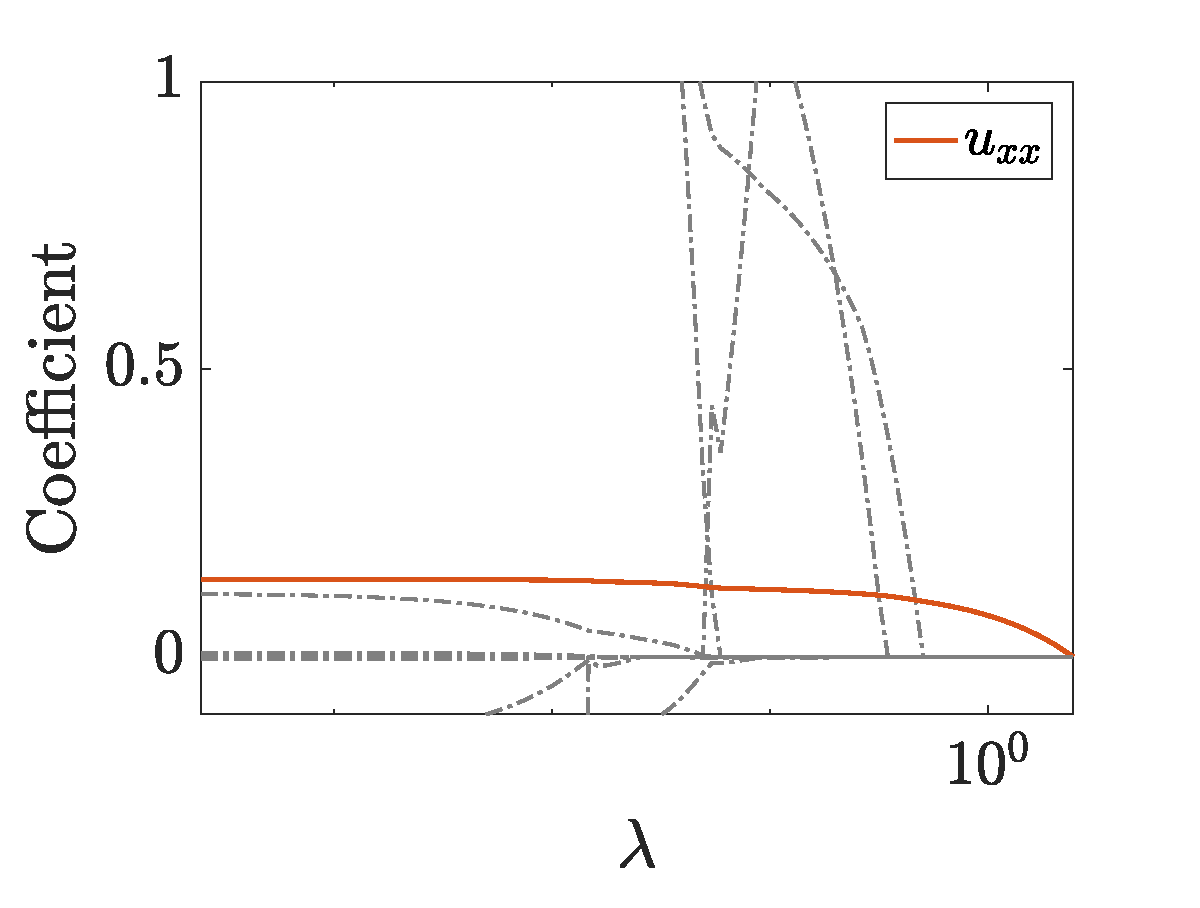
\includegraphics[width=2in]{Figures/heat_0_1.eps}&
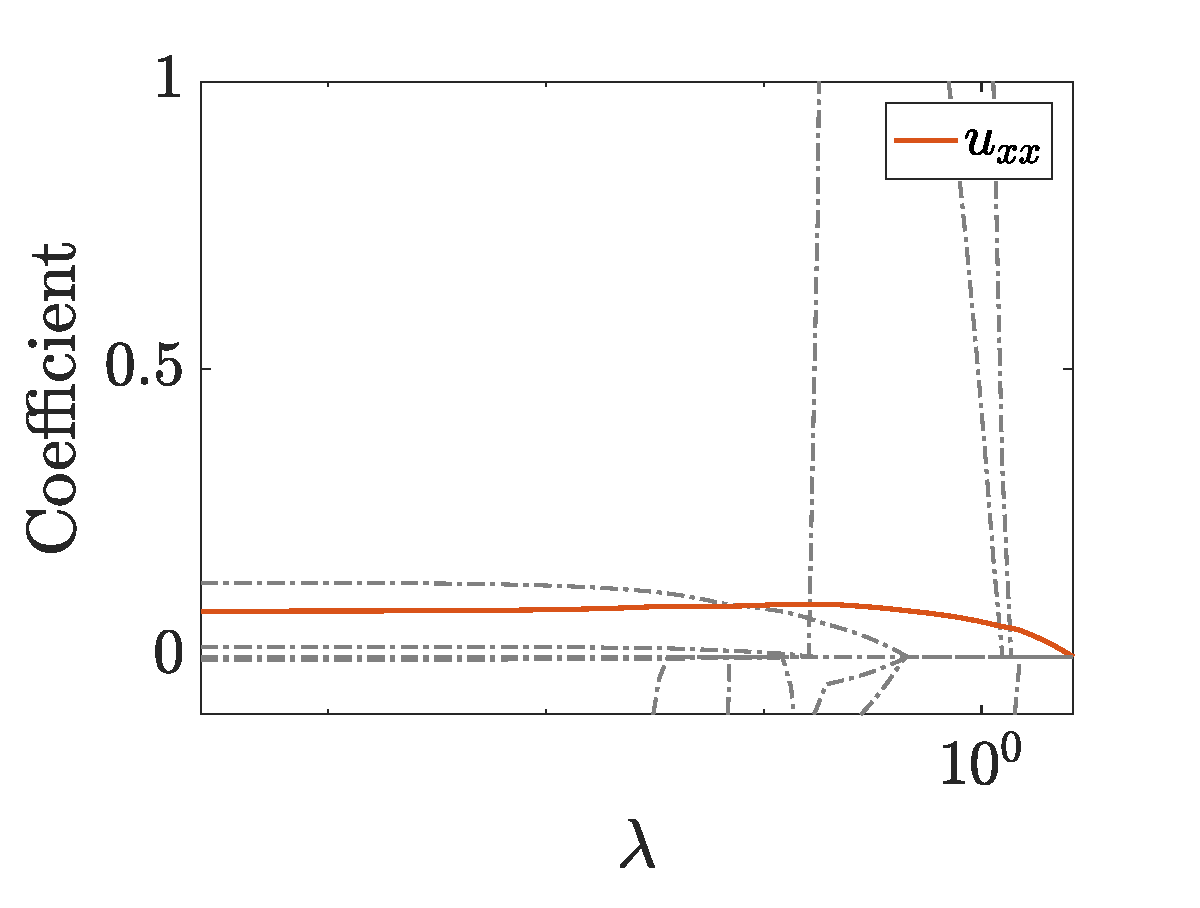
\includegraphics[width=2in]{Figures/heat_0_3.eps}
\end{tabular}	
\caption{[Heat equation] Plots of the coefficients of the candidate feature variables for various parameters $\lambda$ in the $\ell_1$-PsL model under different noise levels: (a) $\sigma=0.01$, (b) $\sigma=0.1$, $\sigma=0.3$. The dashed lines correspond to coefficients of the false feature variables, while the correct one is highlighted by red. As $\lambda$ increases, only the coefficient of the correct feature variable remain non-zero.}\label{expr.heat}
\end{figure}

%\subsubsection{Hyperbolic Equation}
%
%
%\begin{figure}
%\centering
%\begin{tabular}{ccc}
%(a)&(b)&(c)\\
%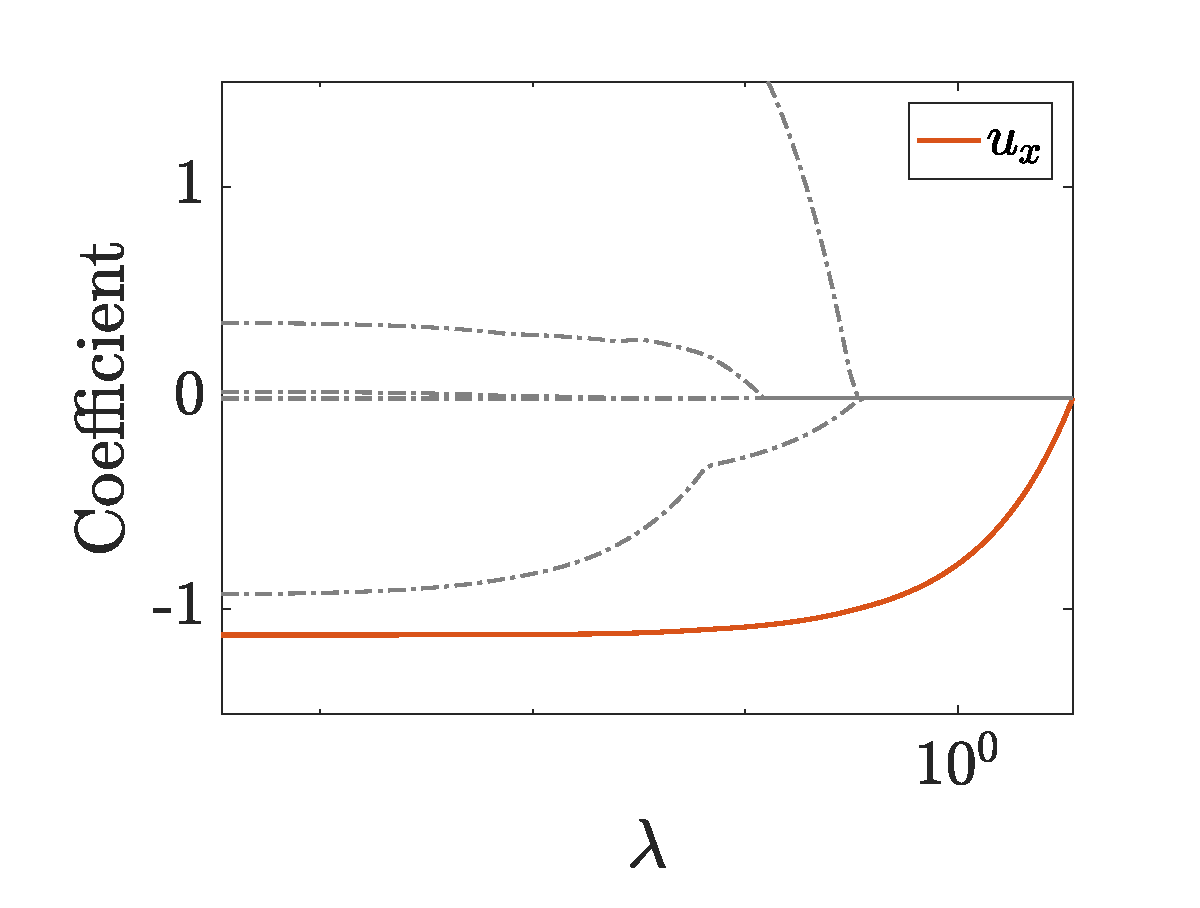
\includegraphics[width=2in]{demotransport_0_5.eps}&
%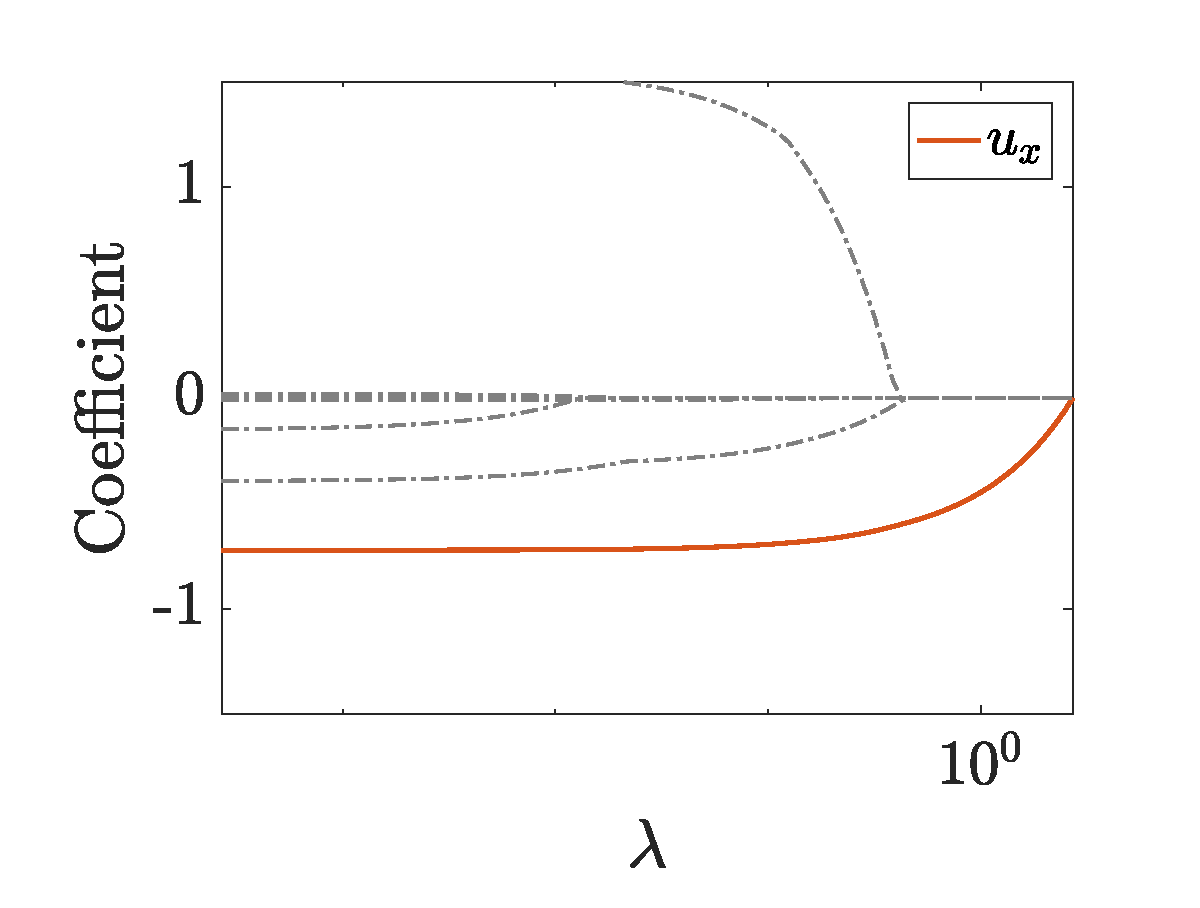
\includegraphics[width=2in]{demotransport_1.eps}&
%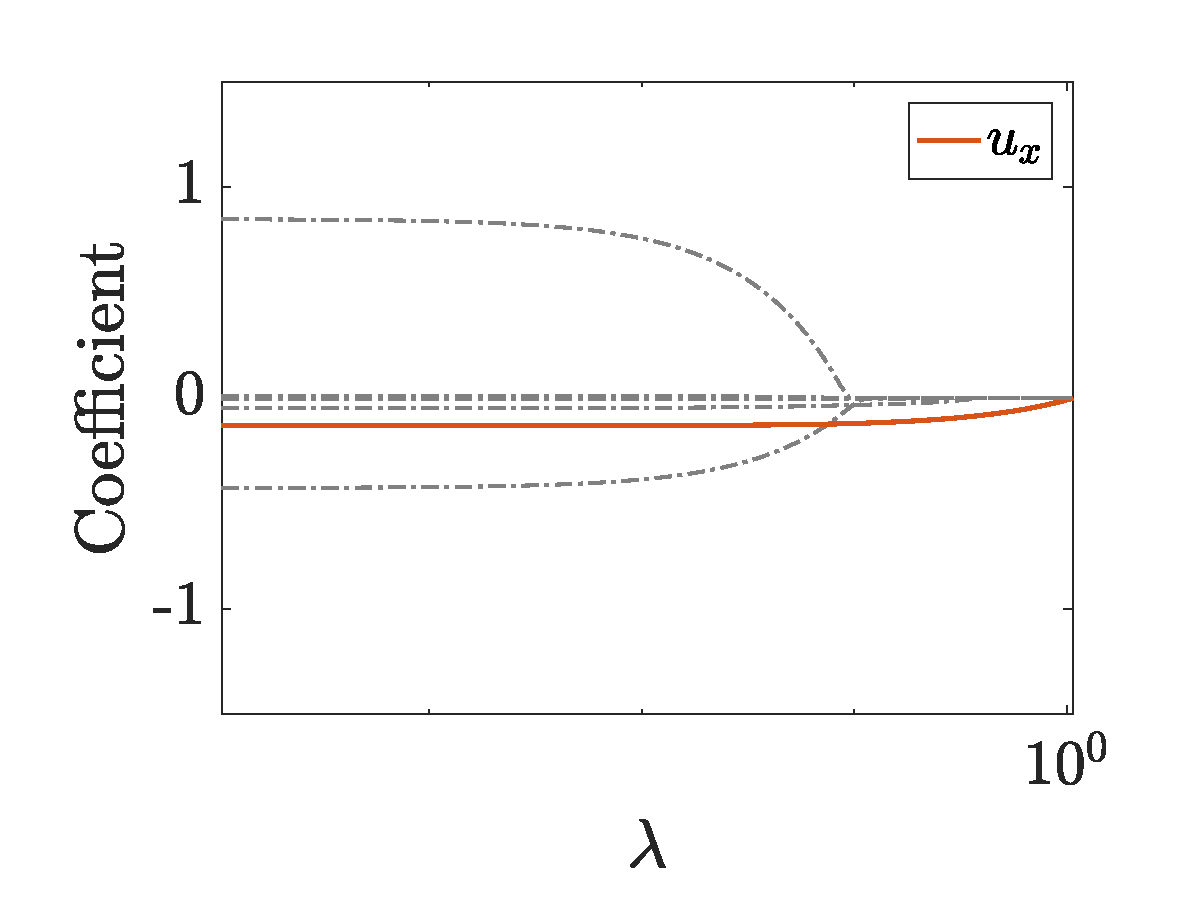
\includegraphics[width=2in]{demotransport_3.eps}
%\end{tabular}	
%\caption{Plots of the coefficients of the candidate feature variables for various parameters $\lambda$ in the $\ell_1$-PsL model under different noise levels: (a) $\sigma=0.01$, (b) $\sigma=0.1$, $\sigma=0.3$. The dashed lines correspond to coefficients of the false feature variables, while the correct one is highlighted by red.}\label{expr.heat}
%\end{figure}


\subsubsection{Burgers' Equation}
Burgers' equation is a simplified Navier-Stokes equation when the pressure gradient is zero. The one-dimensional case equipped with 0-Dirichlet boundary condition is:
\begin{align}
&u_t(x,t) = -(\frac{1}{2}u^2)_x+\nu u_{xx}(x,t)\;,0<x<1,~0<t<T_{\max}\;.\label{eq.burgersPDE}\\
&u(x,0)=f(x)\;, 0\leq x\leq 1\;;\label{eq.burgersPDE.ival}\\
&u(0,t)=u(1,t)=0\;,0\leq t\leq T_{\max}\label{eq.burgersPDE.bd}\;.
\end{align}
When the viscosity coefficient $\nu=0$, the PDE \eqref{eq.burgersPDE}--\eqref{eq.burgersPDE.bd} is often called inviscid Burgers' equation, and it is closely related to the conservation law. If $\nu>0$, then \eqref{eq.burgersPDE}--\eqref{eq.burgersPDE.bd} is referred to as viscous Burgers' equation, which takes the energy dissipation into consideration.

In Figure~\ref{fig.burgers}~(a), we show the numerical solution of the inviscid Burgers' equation with $f(x)=\sin(2\pi x),~0\leq x\leq 1$, $T_{\max}=0.1$, using $\Delta x = 0.01$ and $\Delta t=3.5714\times 10^{-7} (=0.0018/5000)$. We  downsample the solution in times by $5000$, which results in $N=56$ and $M=100$. (b) shows the noisy data ($\sigma=0.3$) and  (c) displays the numerical solution of the PDE identified by $\ell_1$-PsL. The coefficient of the identified feature variable is slightly smaller than the true one; this is due to insufficient time resolution (See Table~\ref{tab.coeff.burgers}) and the smoothing effects of the local polynomial regression technique. Figure~\ref{expr.burgers} shows the dependence of the coefficients of the candidate feature variables on the choice of $\lambda$. As the noise increases, the coefficient of the correct feature variable becomes less accurate, and those of the false feature variables becomes more significant.
\begin{table}
\centering
\begin{tabular}{c|c|c|c}
Time resolution $(N_0=100^{7/8})$&$N_0$&$10N_0$&$100N_0$\\\hline
Estimated coefficient for $uu_x$&$-0.6794$&$-0.7499$&$-0.8005$
\end{tabular}	
\caption{[Inviscid Burgers' equation] Increased time resolution results in higher accuracy of the estimated coefficient of the identified feature variable: $uu_x$ in the inviscid Burgers' equation. The true value is $-1$, and the space resolution is remained at $M=100$.}\label{tab.coeff.burgers}
\end{table}


\begin{figure}
\centering
\begin{tabular}{ccc}
(a)&(b)&(c)\\
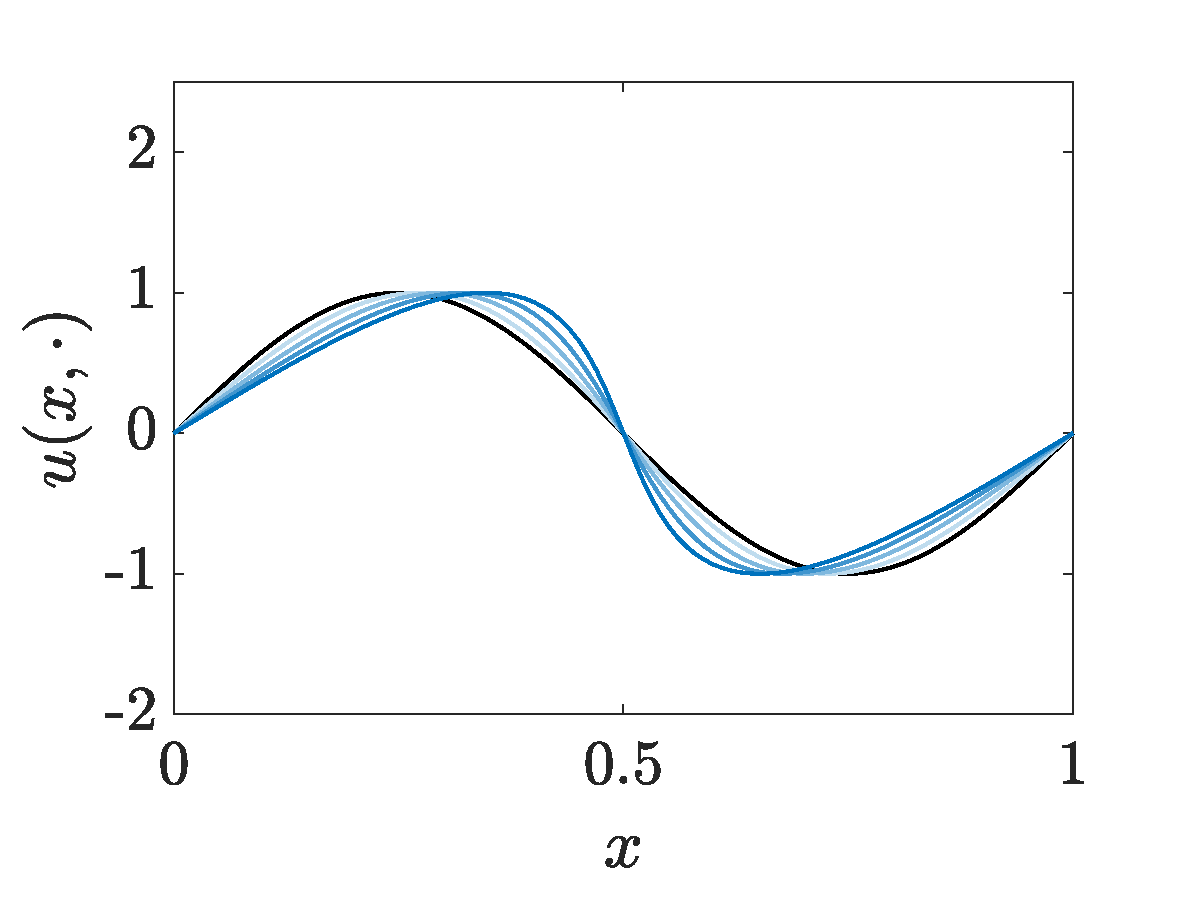
\includegraphics[width=2in]{Figures/burgers_sol.eps}&
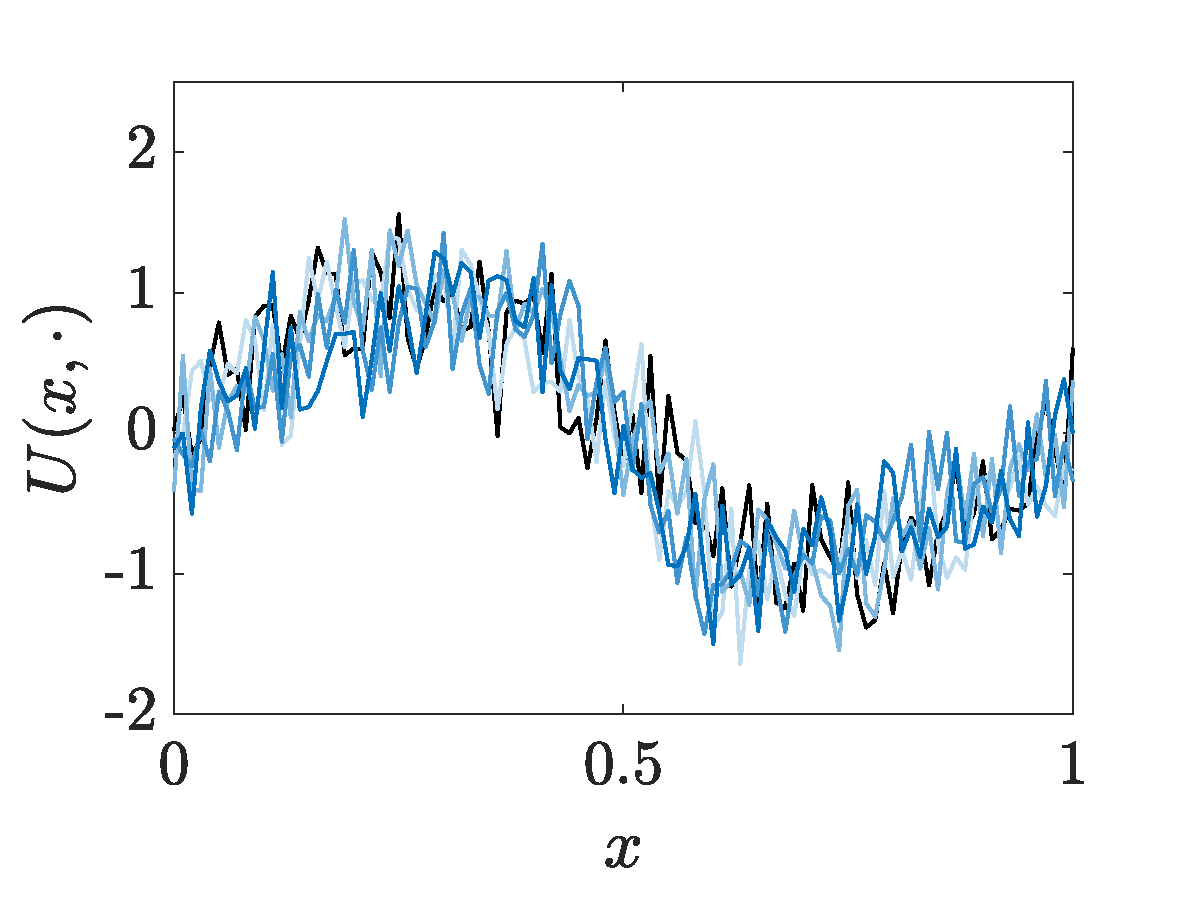
\includegraphics[width=2in]{Figures/burgers_noise.eps}&
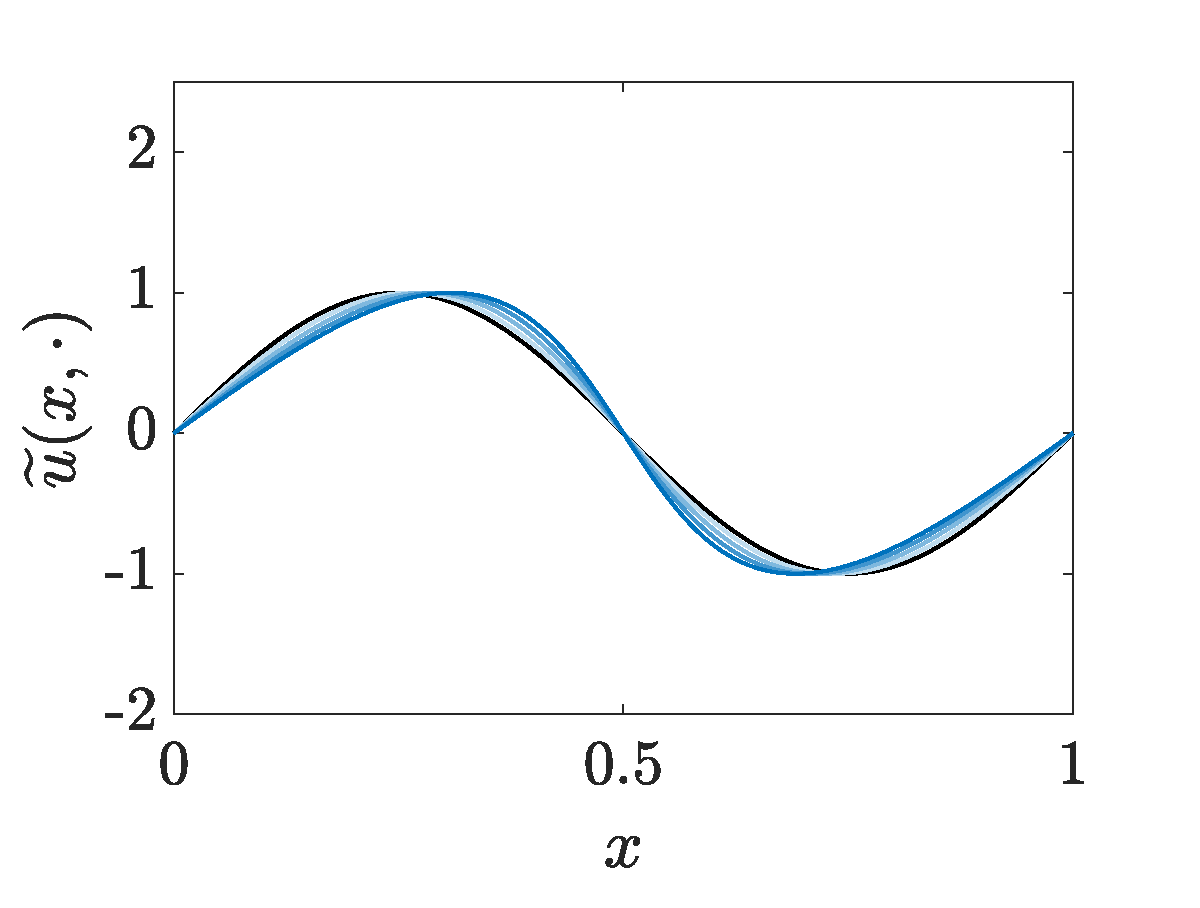
\includegraphics[width=2in]{Figures/burgers_resimul.eps}
\end{tabular}
\caption{[Inviscid Burgers' equation] (a) Numerical solution of the inviscid Burgers' equation: $u_t=-uu_{xx}$ with initial condition: $f(x)=\sin(2\pi x),~0\leq x\leq 1$. (b) Data obtained from (a) with additive Gaussian noise of intensity $\sigma=0.3$. (c) Numerical solution of the identified PDE: $u_t=-0.5946uu_{x}$. }	\label{fig.burgers}
\end{figure}

\begin{figure}
\centering
\begin{tabular}{ccc}
(a)&(b)&(c)\\
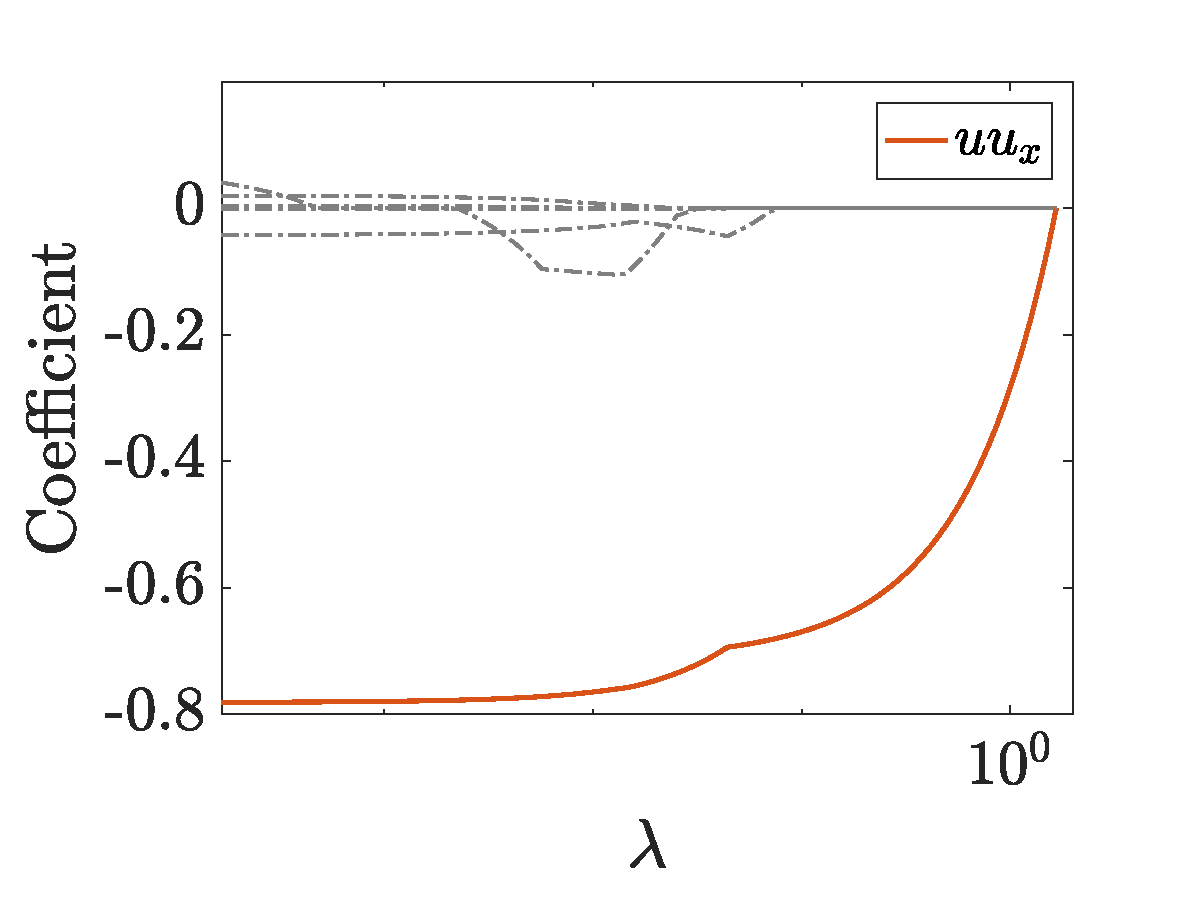
\includegraphics[width=2in]{Figures/burgers_0_1.eps}&
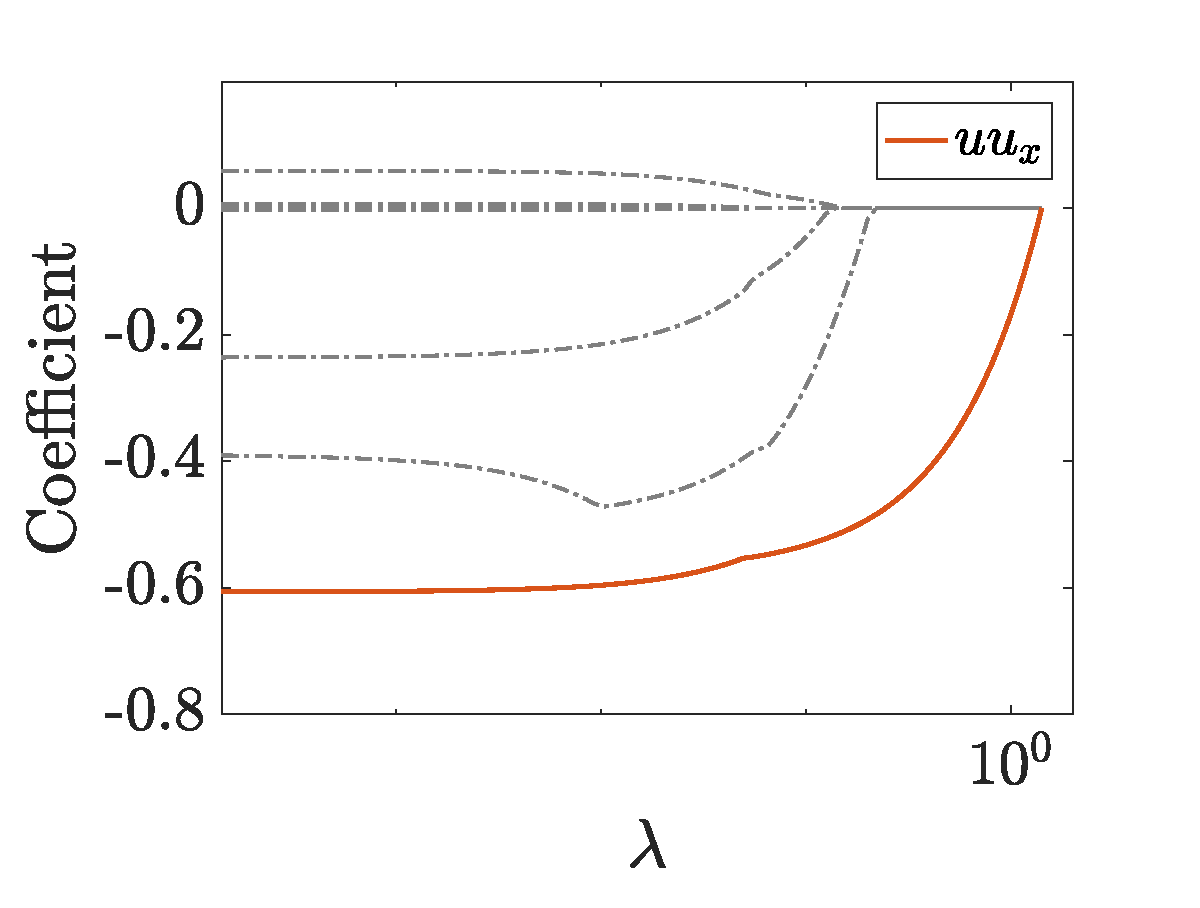
\includegraphics[width=2in]{Figures/burgers_0_5.eps}&
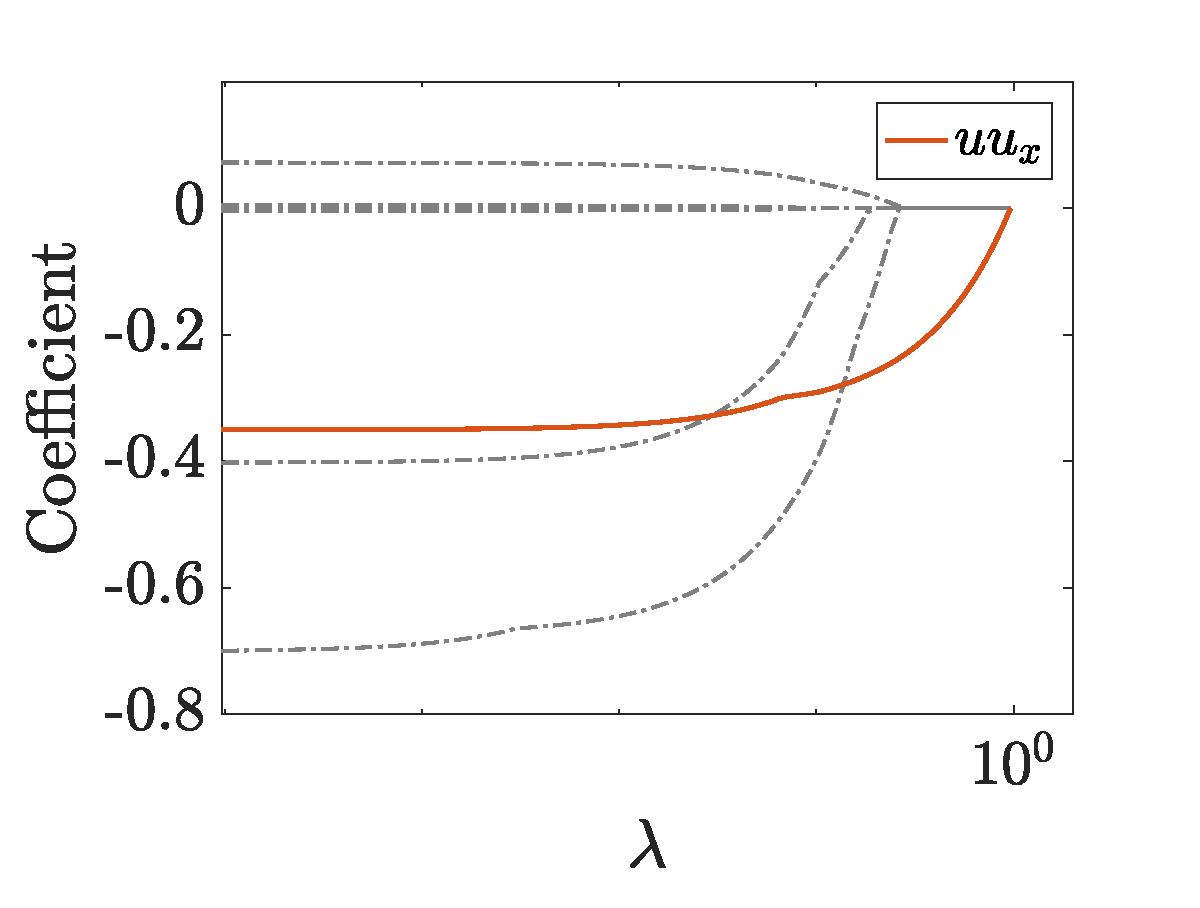
\includegraphics[width=2in]{Figures/burgers_1.eps}
\end{tabular}	
\caption{[Inviscid Burgers' equation] Plots of the coefficients of the candidate feature variables for various parameters $\lambda$ in the $\ell_1$-PsL model under different noise levels: (a) $\sigma=0.1$, (b) $\sigma=0.5$, $\sigma=1.0$. The dashed lines correspond to coefficients of the false feature variables, while the correct one is highlighted by red.}\label{expr.burgers}
\end{figure}


Figure~\ref{fig.visburgers}~(a) shows the numerical solution of the viscous Burgers' equation with $f(x)=\sin^2(4\pi x)+\sin^3(2\pi x),~0\leq x\leq 1$, $T_{\max}=0.1$, and $\nu=0.01$, while keeping the grid same as above. (b) shows the noisy data ($\sigma=0.5$) and (c) displays the  solution of the PDE identified by $\ell_1$-PsL. Higher level of noise submerges the shock formation determined by the feature $uu_x$, and the smoothing effects of the local polynomial regression analogous to the diffusion term $u_{xx}$ becomes obvious. This is clear in Figure~\ref{expr.visburgers}. After all the false feature variables have vanished, when the noise increases, $\ell_1$-PsL filters out the feature $u_{xx}$ later than $uu_x$.
\begin{figure}
\centering
\begin{tabular}{ccc}
(a)&(b)&(c)\\
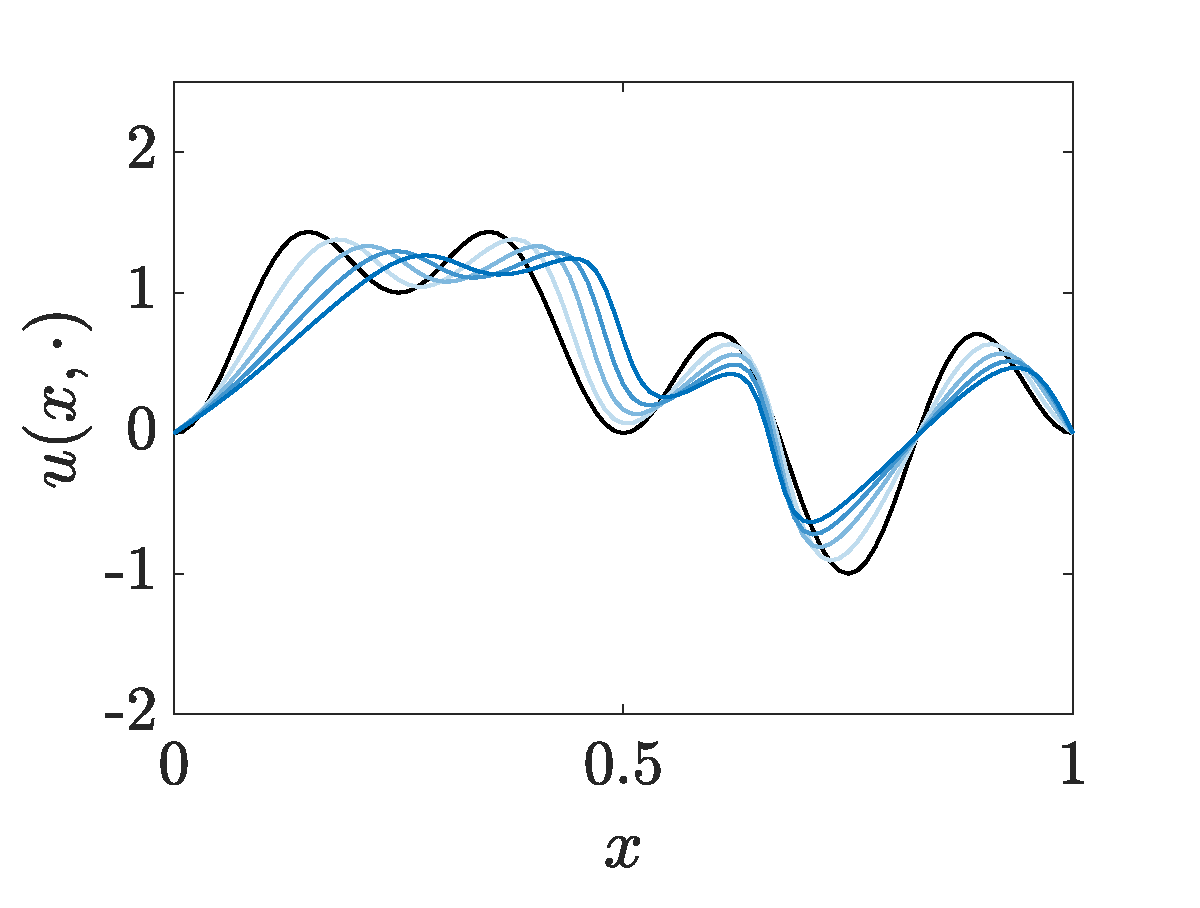
\includegraphics[width=2in]{Figures/visburgers_sol.eps}&
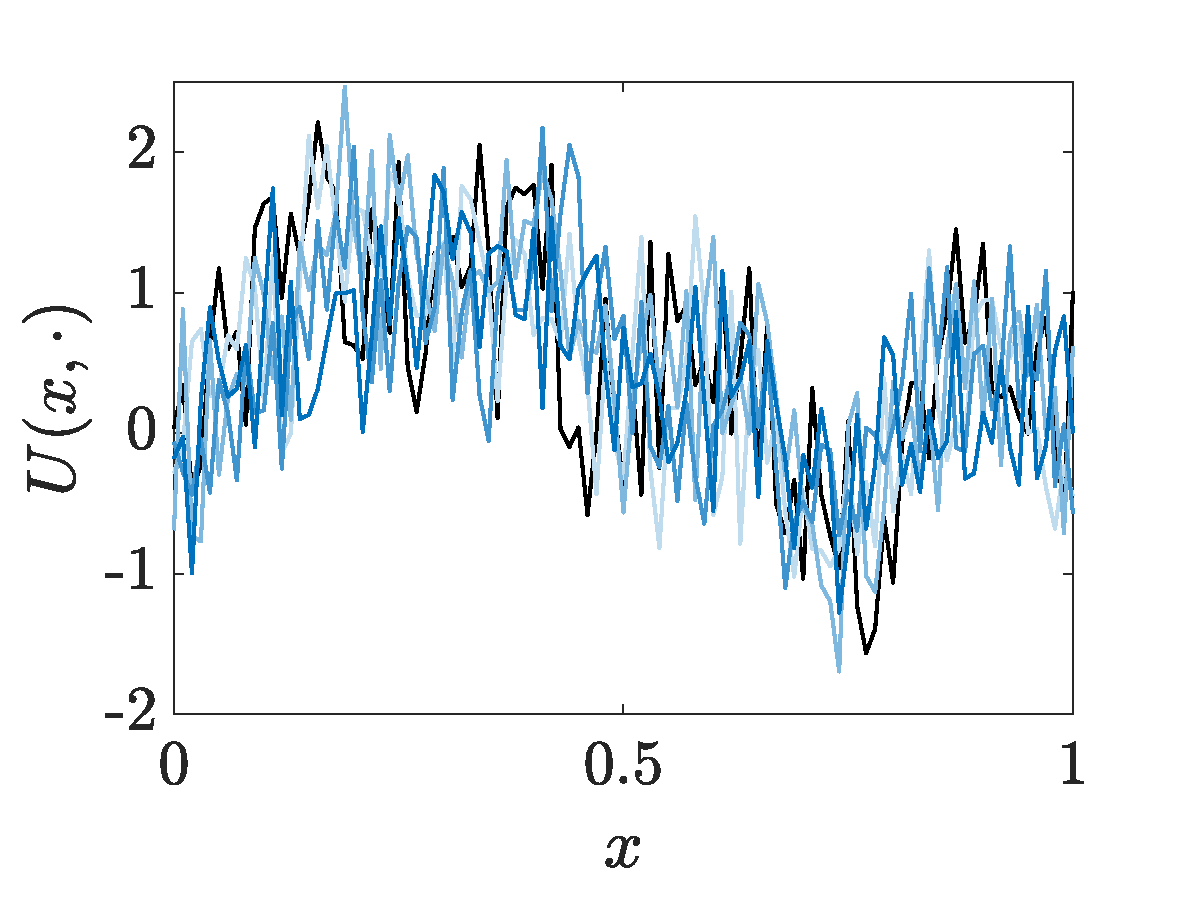
\includegraphics[width=2in]{Figures/visburgers_noise.eps}&
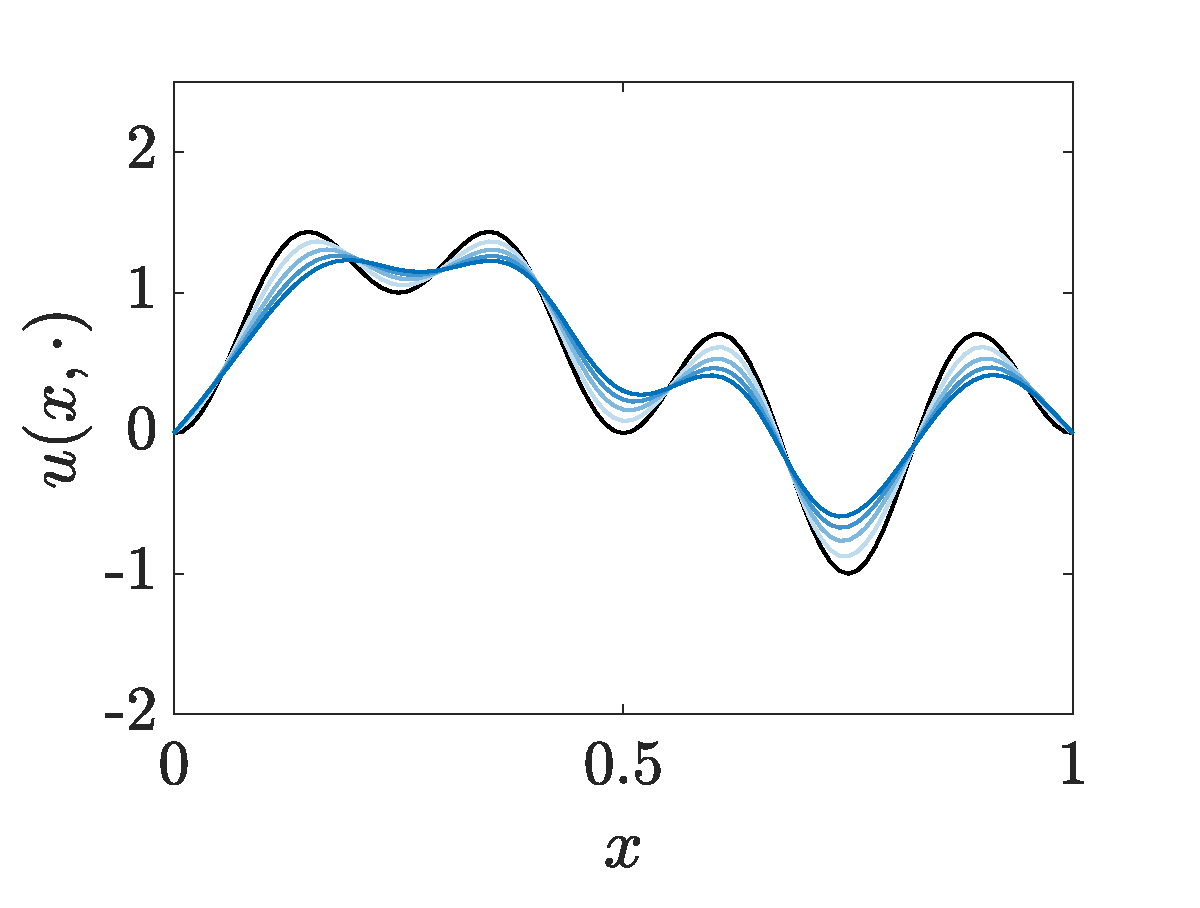
\includegraphics[width=2in]{Figures/visburgers_resimul.eps}
\end{tabular}
\caption{[Viscous Burgers' equation] (a) Numerical solution of the viscous Burgers' equation: $u_t=-uu_{x}+0.01u_{xx}$ with initial condition: $f(x)=\sin^2(4\pi x)+\sin^3(2\pi x);,~0\leq x\leq 1$. (b) Data obtained from (a) with additive Gaussian noise of intensity $\sigma=0.5$. (c) Numerical solution of the identified PDE: $u_t=-0.2115uu_{x}+0.0131u_{xx}$. }	\label{fig.visburgers}
\end{figure}
\begin{figure}
\centering
\begin{tabular}{ccc}
(a)&(b)&(c)\\
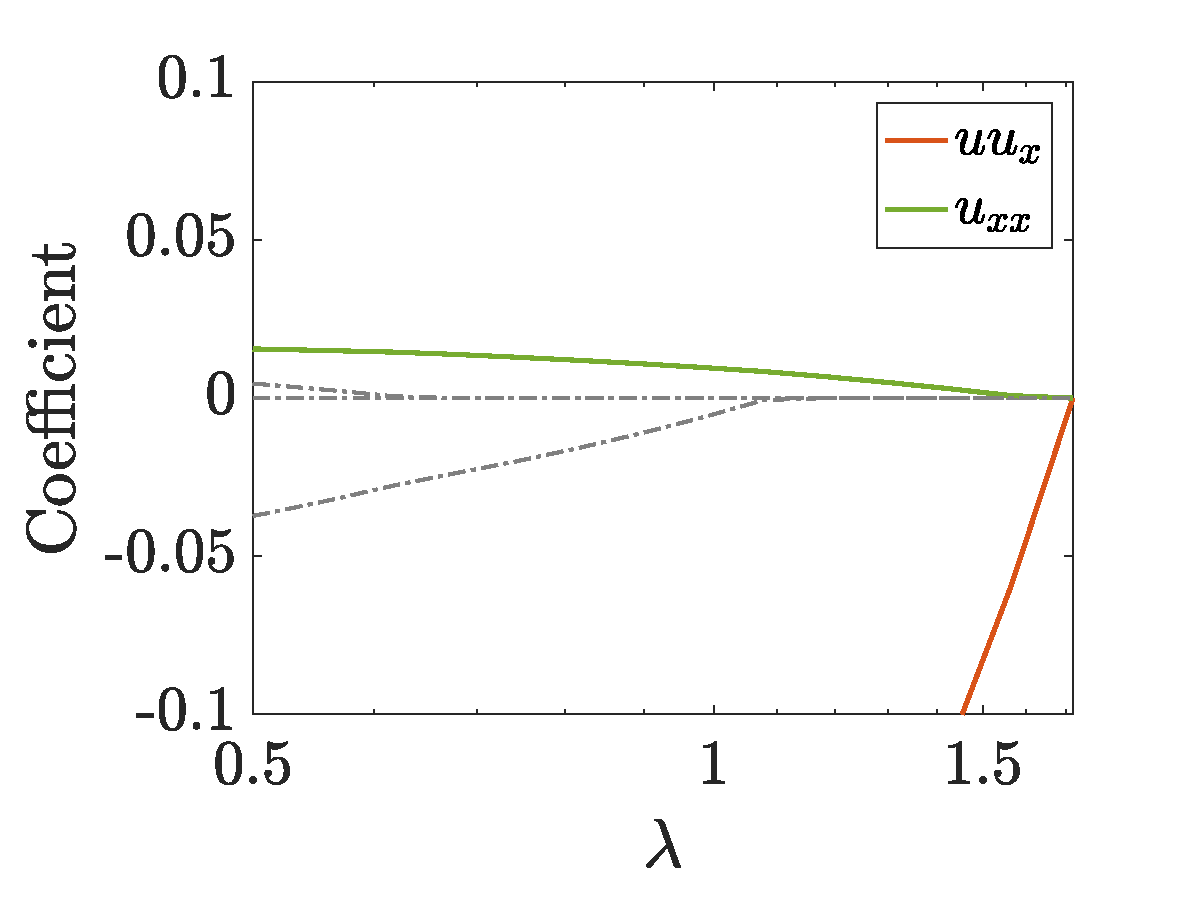
\includegraphics[width=2in]{Figures/visburgers_0_1.eps}&
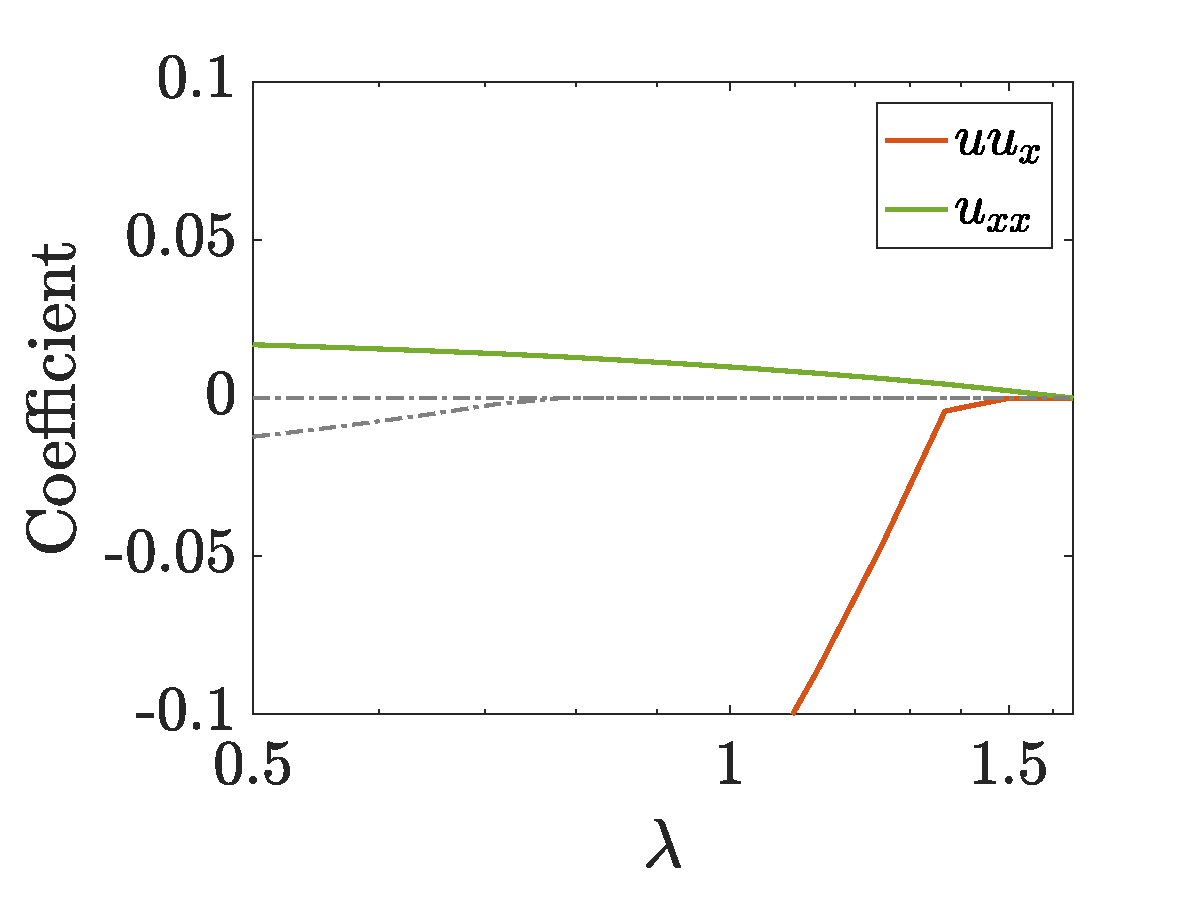
\includegraphics[width=2in]{Figures/visburgers_0_5.eps}&
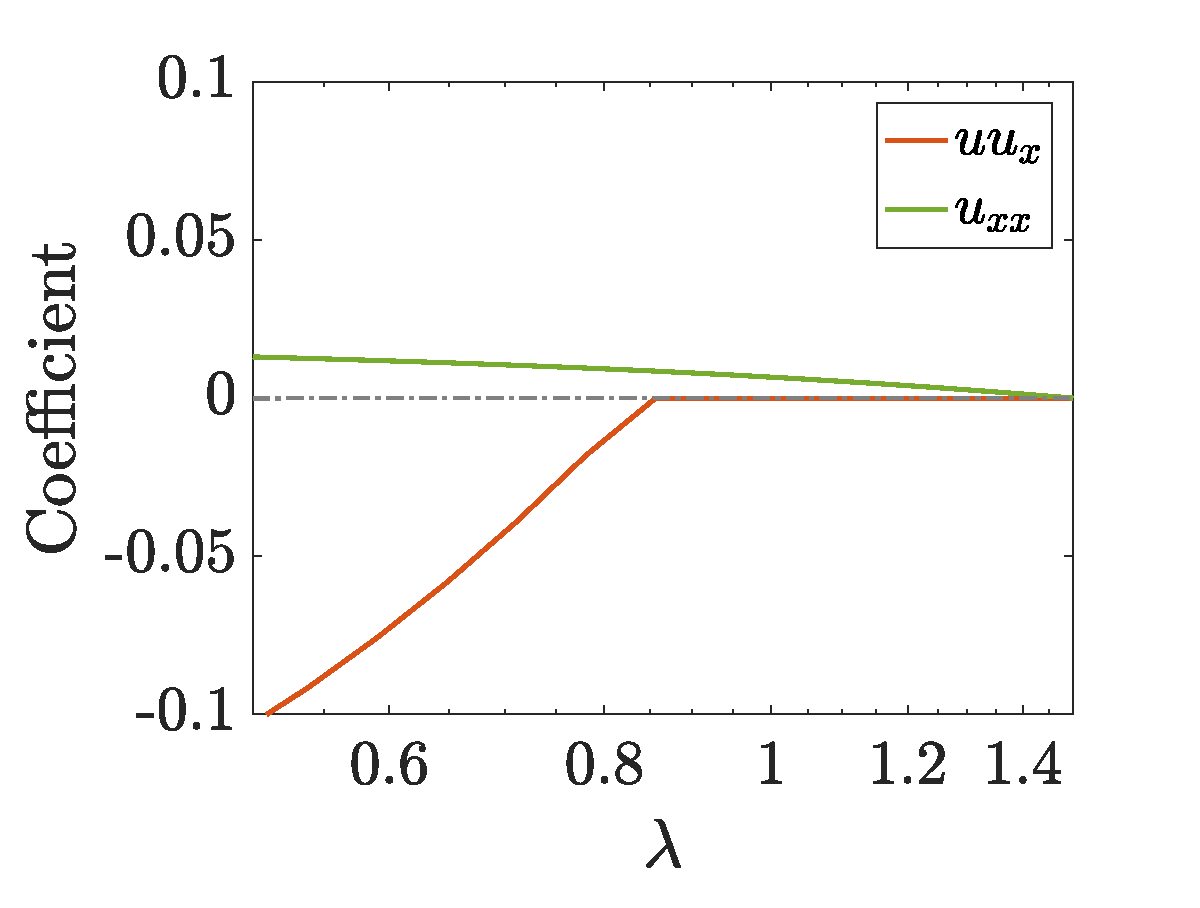
\includegraphics[width=2in]{Figures/visburgers_1.eps}
\end{tabular}	
\caption{[Viscous Burgers' equation] Plots of the coefficients of the candidate feature variables for various parameters $\lambda$ in the $\ell_1$-PsL model under different noise levels: (a) $\sigma=0.1$, (b) $\sigma=0.5$, and (c) $\sigma=1.0$. Here we focus on the range of $\lambda$ where the false feature variables have vanished. The dashed lines correspond to coefficients of the false feature variables, while the correct ones are highlighted by red and green.}\label{expr.visburgers}
\end{figure}



%\subsection{General Behavior of $\ell_1$-PsL based PDE Identification}
%Figure~\ref{expr.transport} for transport equation. Figure~\ref{expr.transport} for advection-diffusion equation.
%\begin{figure}
%\centering
%\begin{tabular}{ccc}
%(a)&(b)&(c)\\
%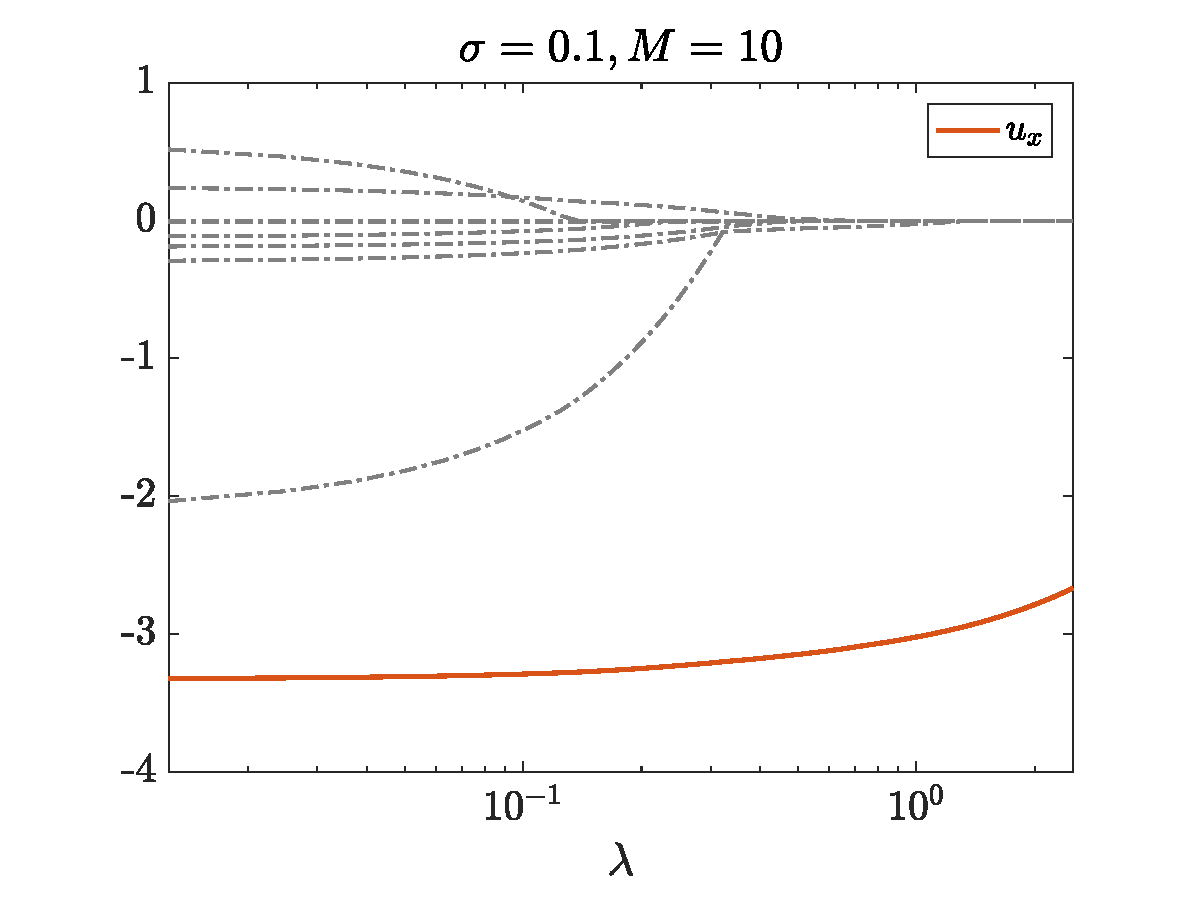
\includegraphics[width=2in]{transportExp1_10_0_1.eps}&
%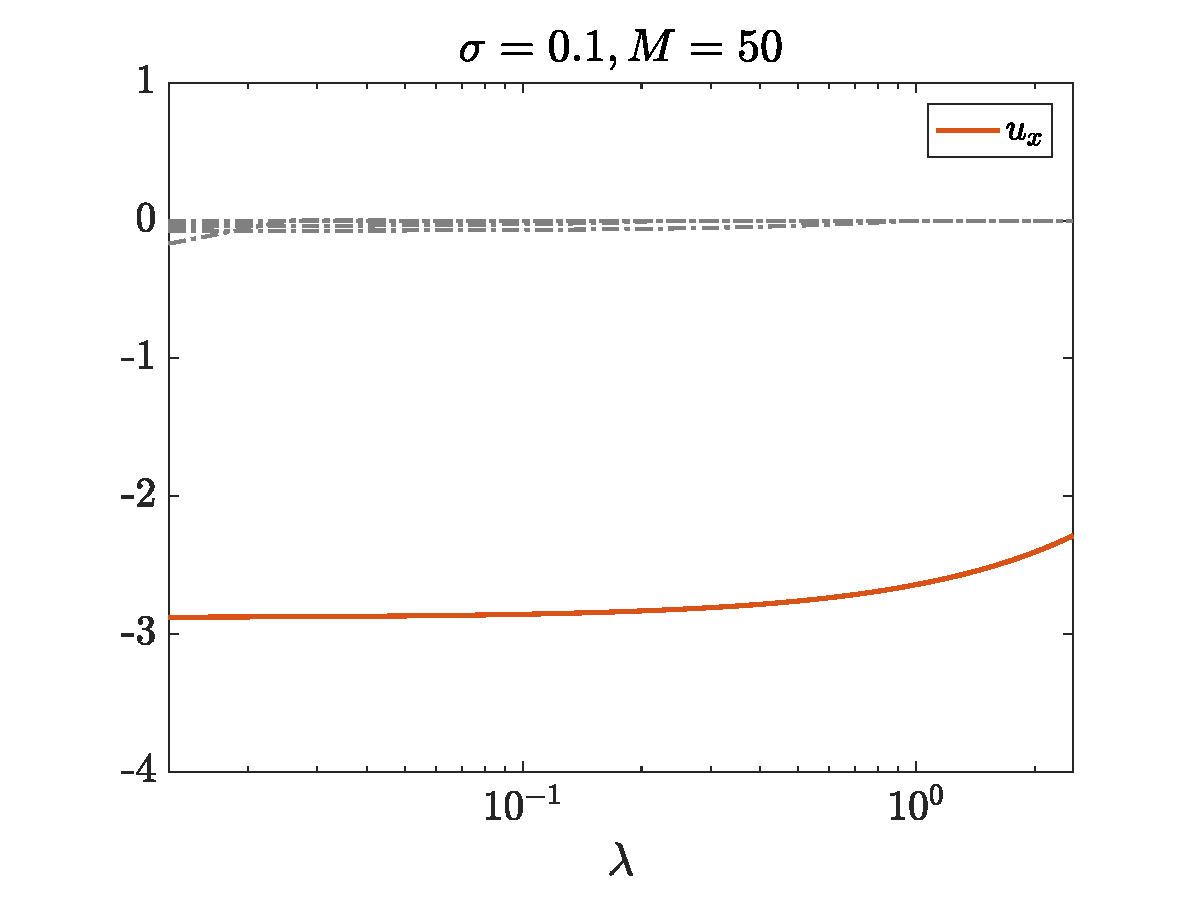
\includegraphics[width=2in]{transportExp1_50_0_1.eps}&
%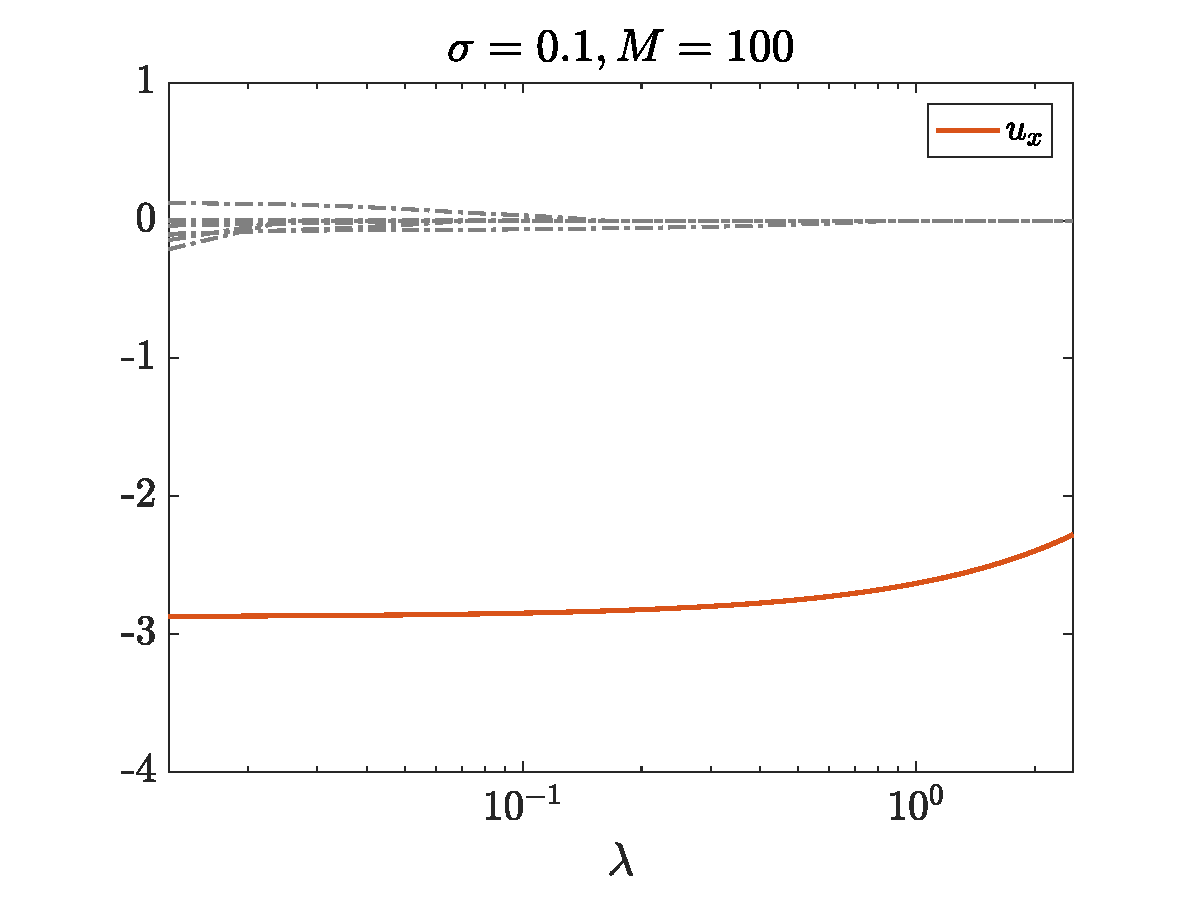
\includegraphics[width=2in]{transportExp1_100_0_1.eps}\\
%(d)&(e)&(f)\\
%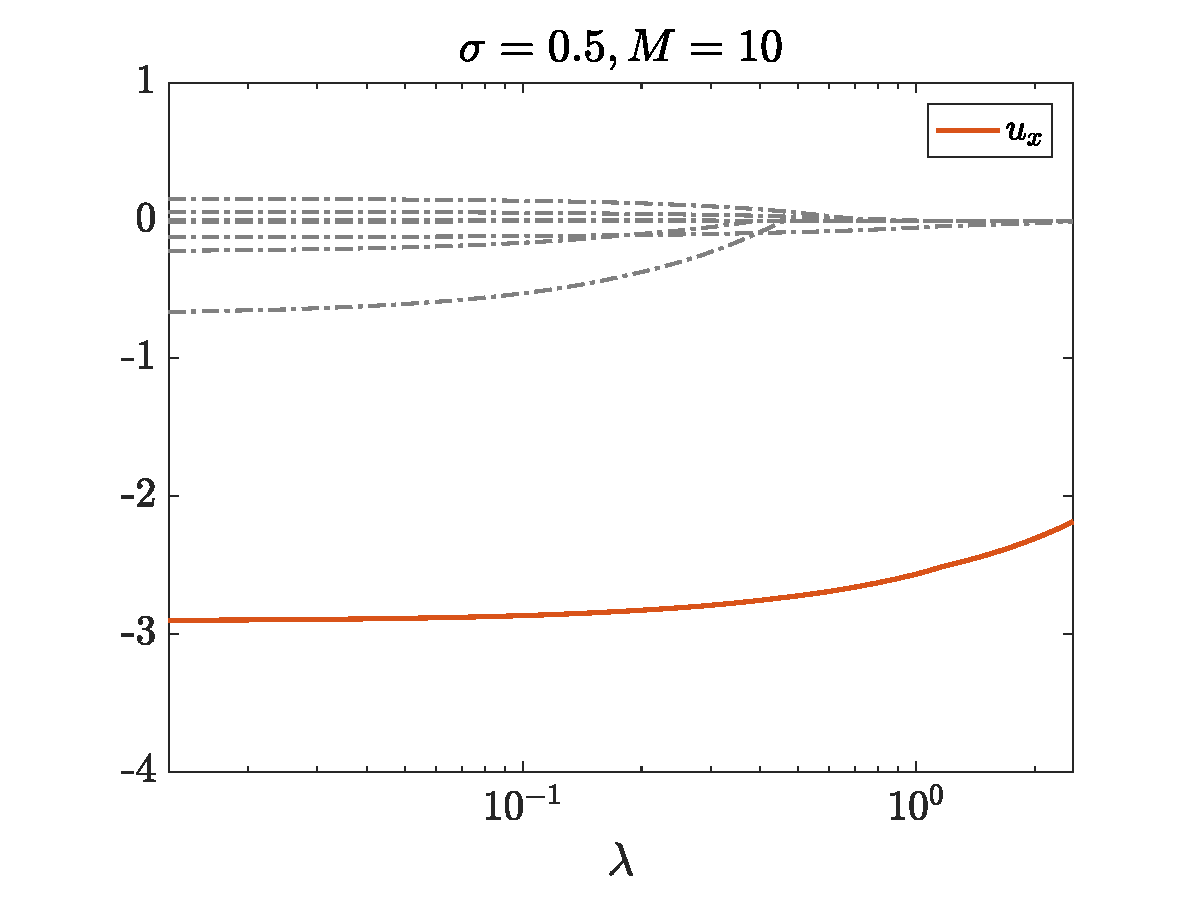
\includegraphics[width=2in]{transportExp1_10_0_5.eps}&
%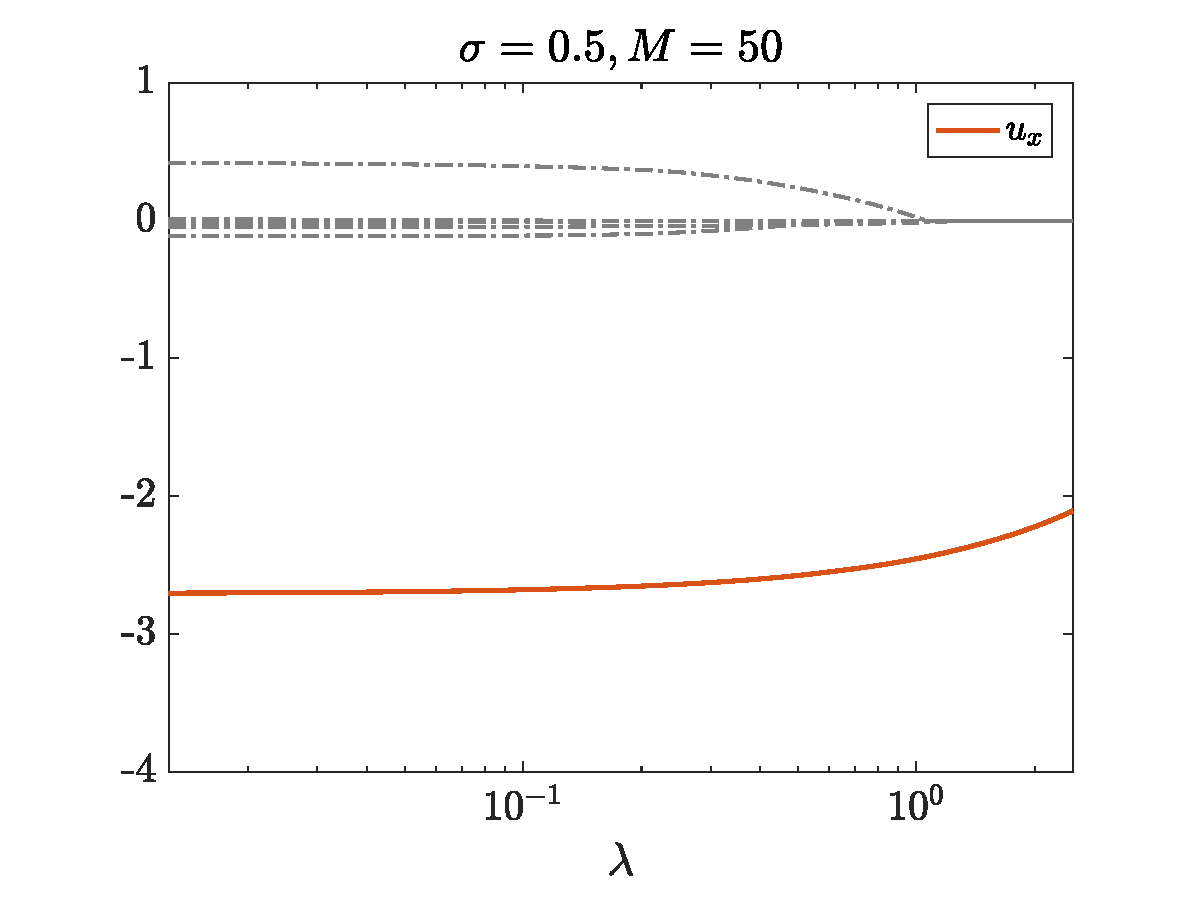
\includegraphics[width=2in]{transportExp1_50_0_5.eps}&
%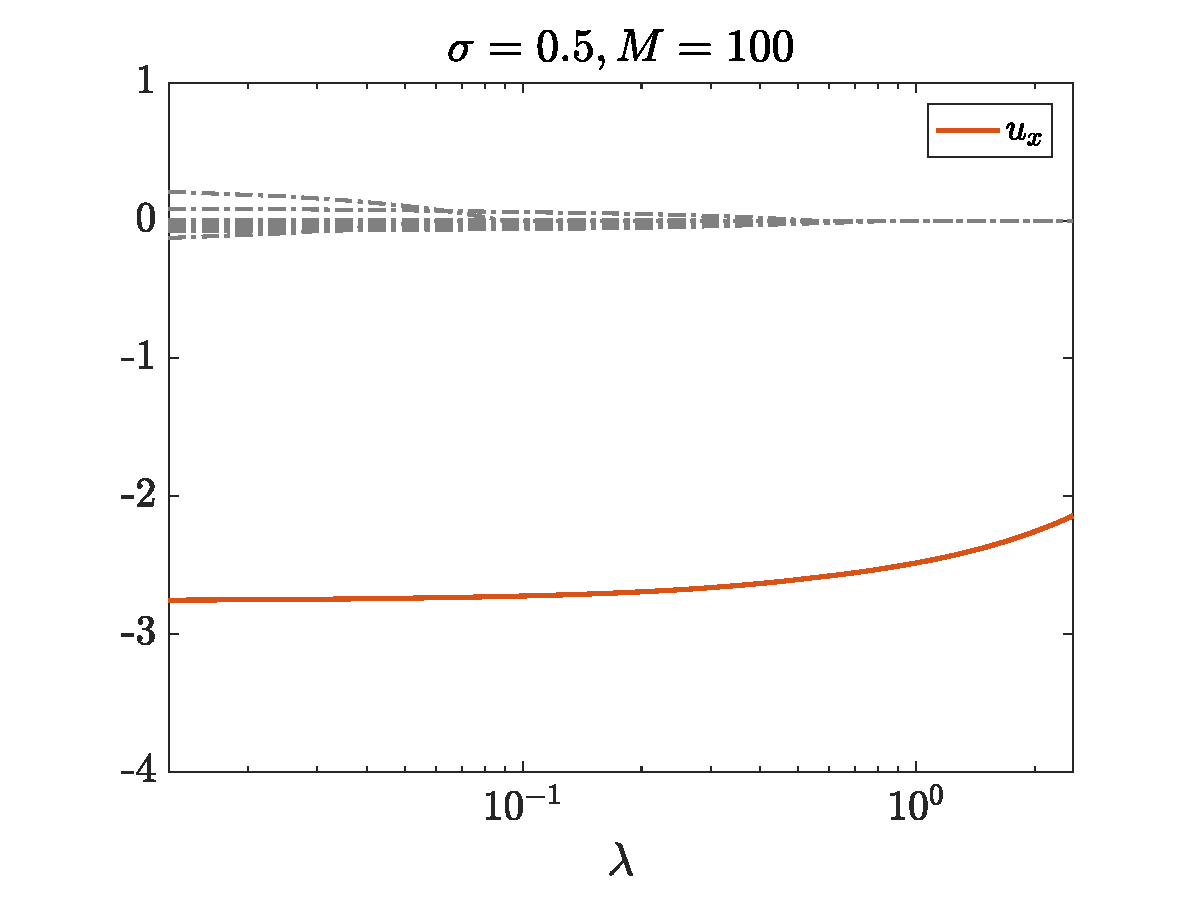
\includegraphics[width=2in]{transportExp1_100_0_5.eps}
%\end{tabular}	
%\caption{$\ell_1$-PsL model for PDE identification when the underlying PDE is transport equation: $u_t=-(8/3)u_x$ with an observed function: $u(x,t)=2\sin(3x-8t)$, $0\leq x\leq 1$, $0\leq t\leq 2$. (a) $\sigma=0.1, N=10$; (b) $\sigma=0.1, N=50$; (c) $\sigma=0.5, N=100$. (d) $\sigma=0.5, N=10$; (e) $\sigma=0.1, N=50$; (f) $\sigma=0.5, N=100$.}\label{expr.transport}
%\end{figure}
%
%
%\begin{figure}
%\centering
%\begin{tabular}{ccc}
%(a)&(b)&(c)\\
%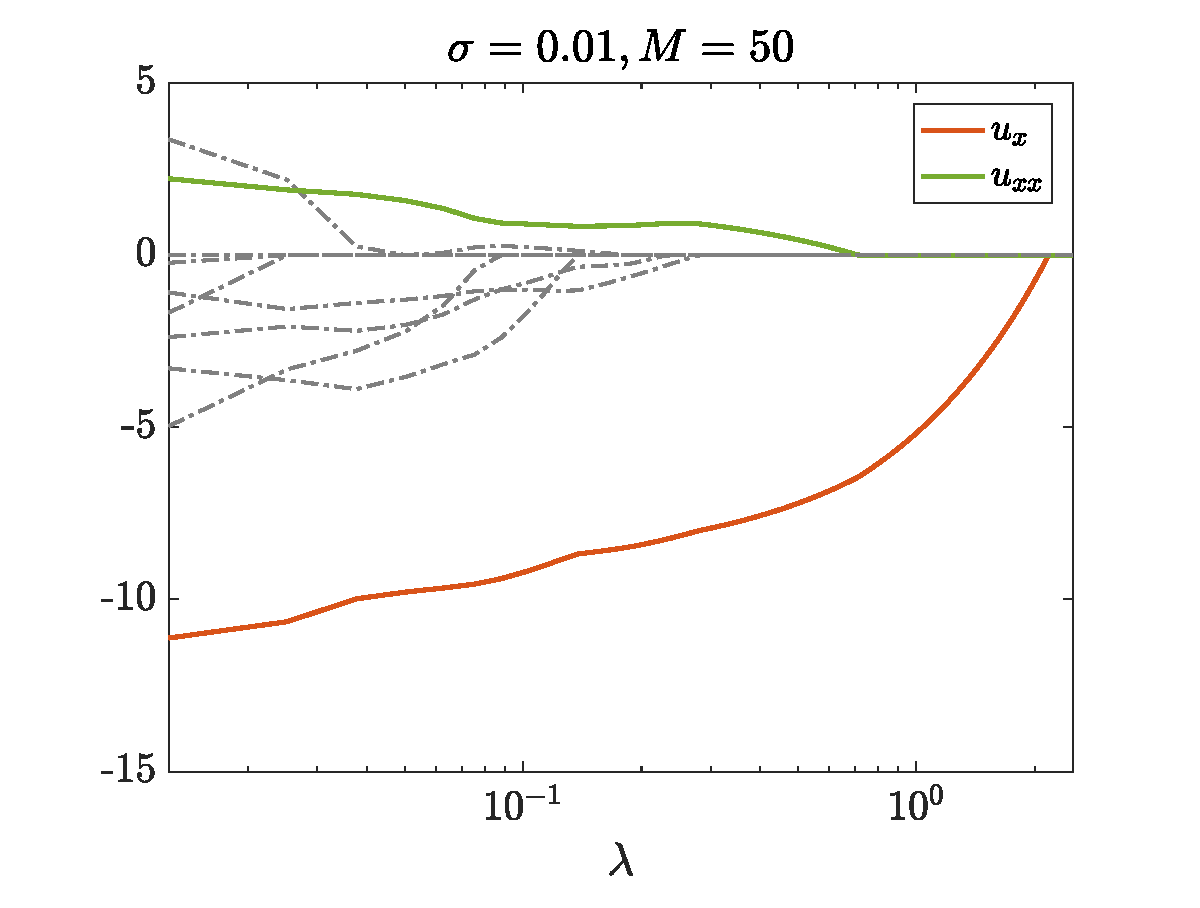
\includegraphics[width=2in]{advdiffExp1_50_0_01.eps}&
%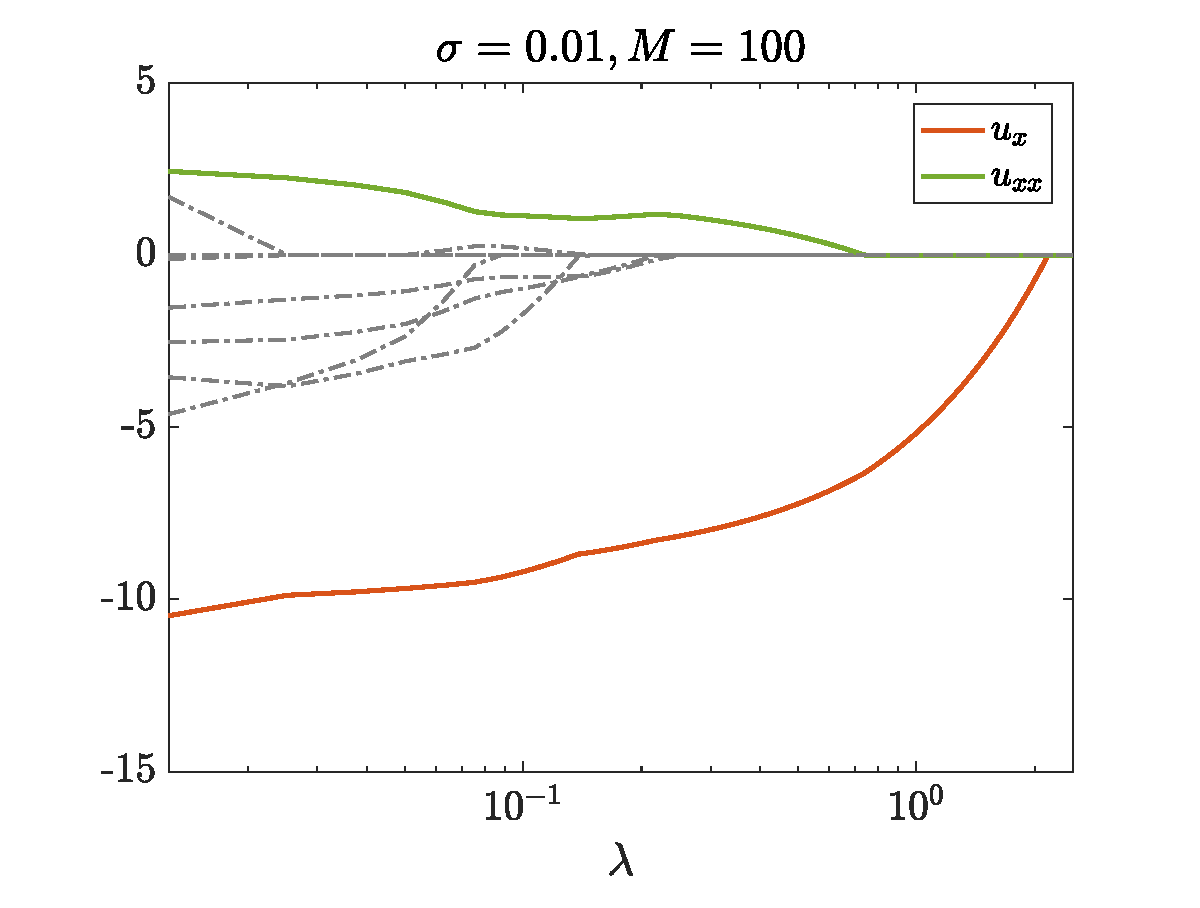
\includegraphics[width=2in]{advdiffExp1_100_0_01.eps}&
%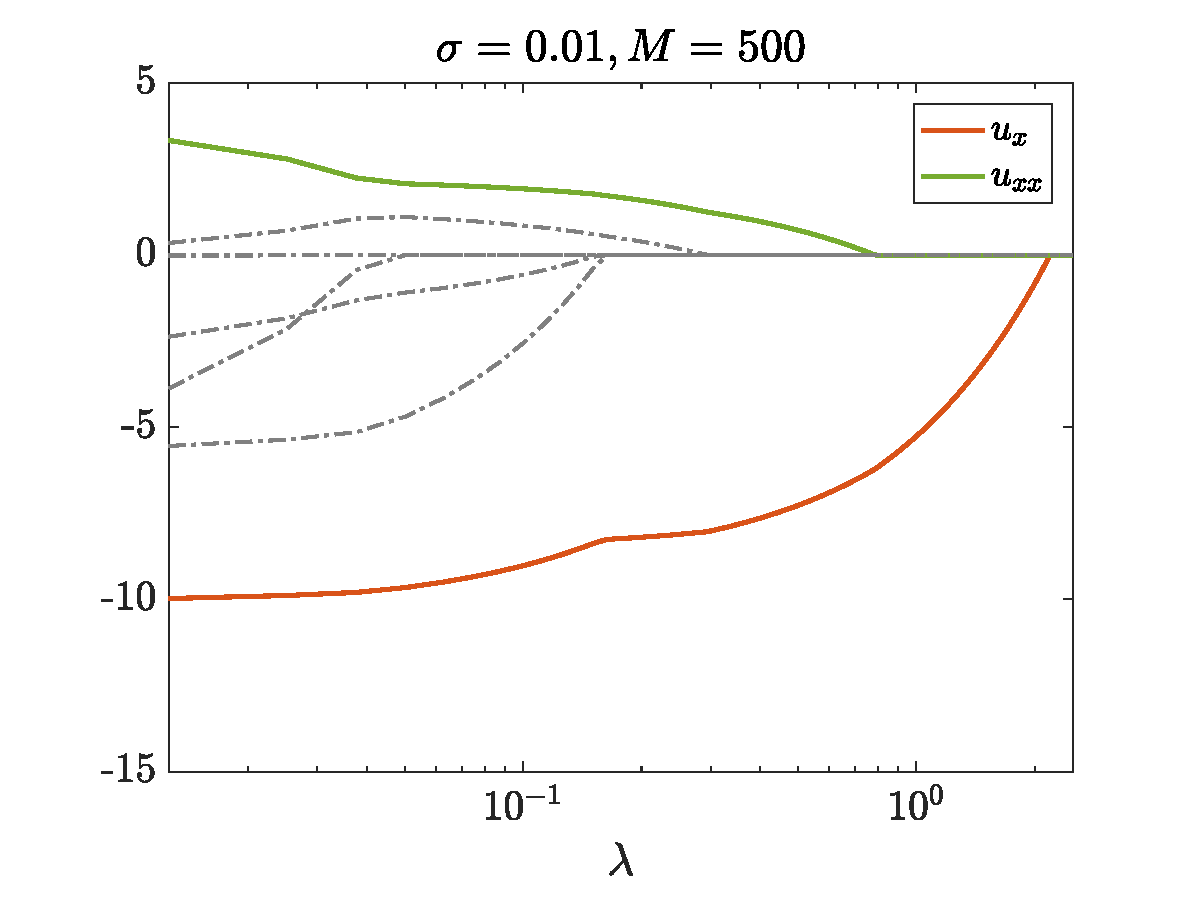
\includegraphics[width=2in]{advdiffExp1_500_0_01.eps}\\
%(d)&(e)&(f)\\
%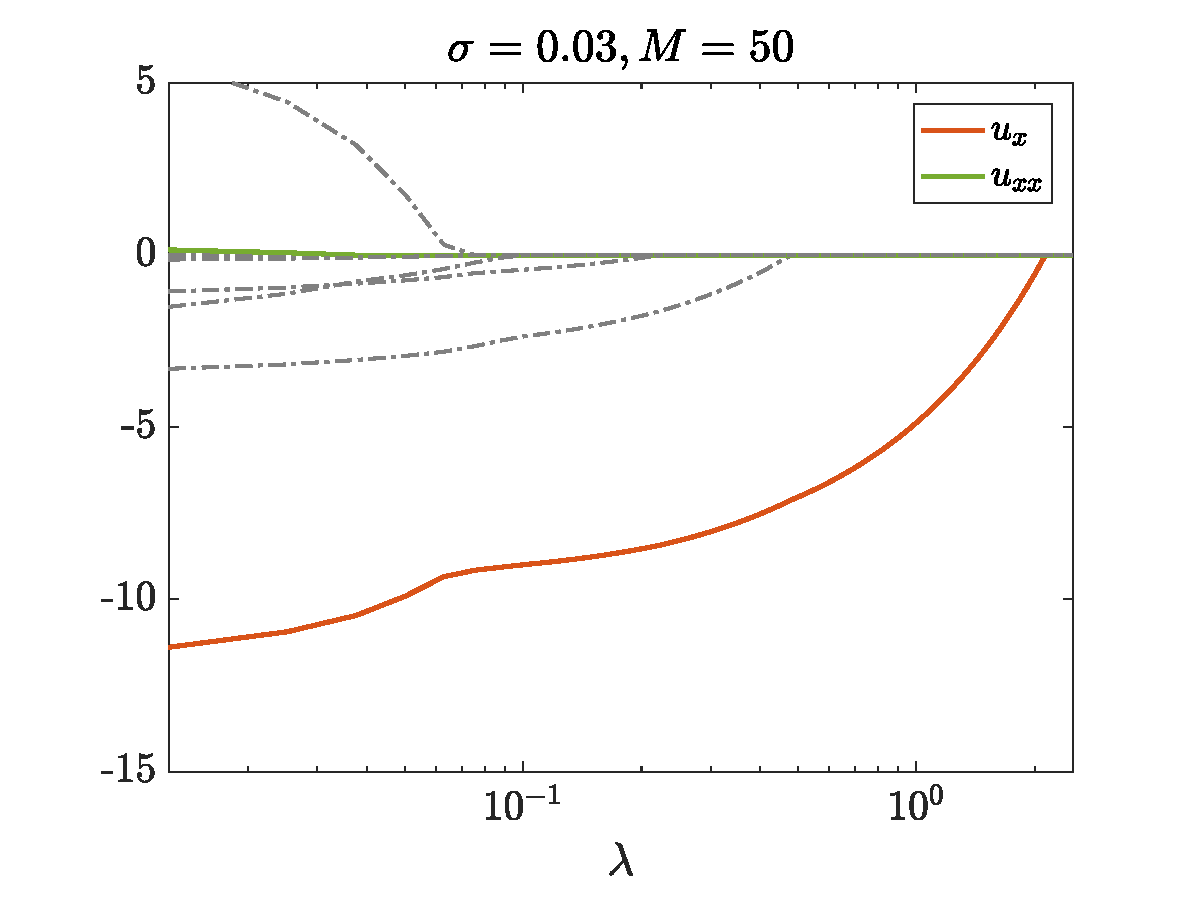
\includegraphics[width=2in]{advdiffExp1_50_0_03.eps}&
%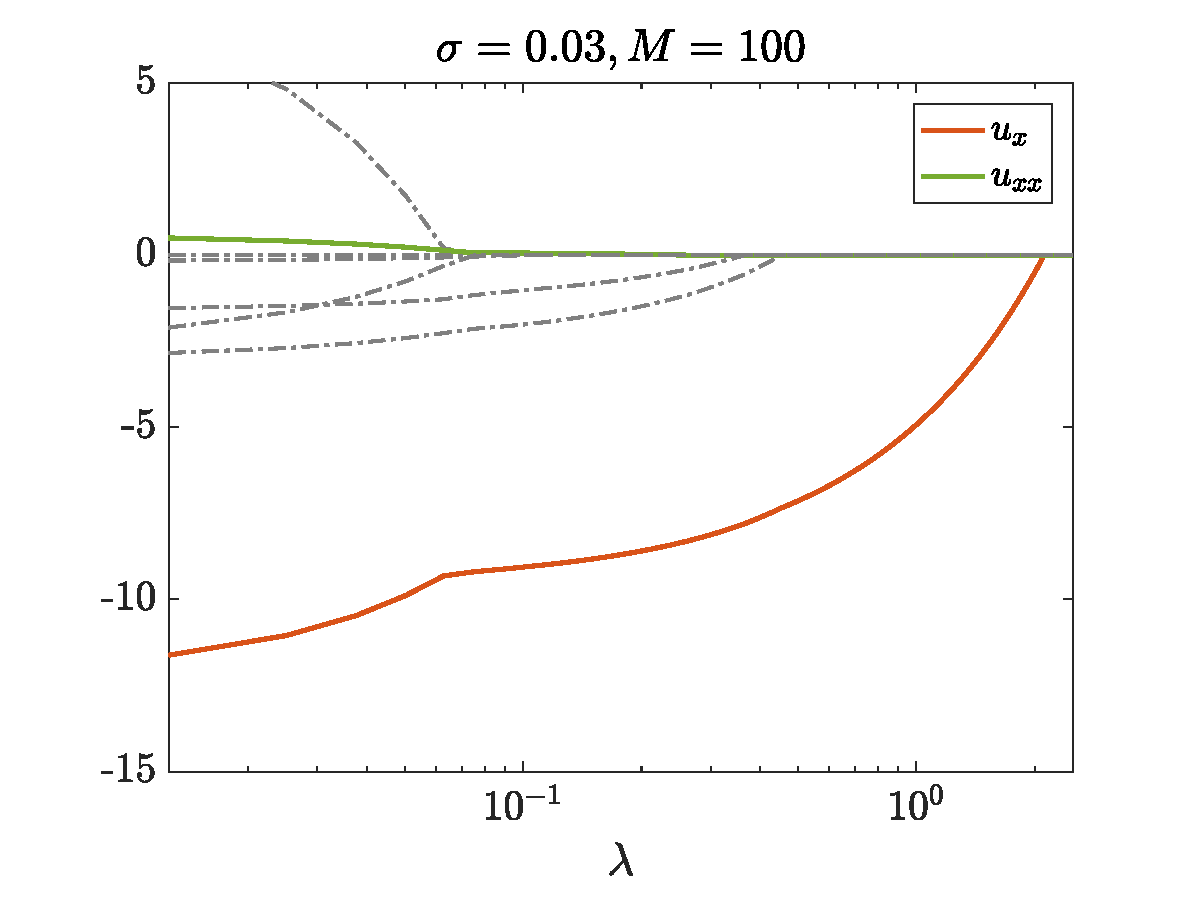
\includegraphics[width=2in]{advdiffExp1_100_0_03.eps}&
%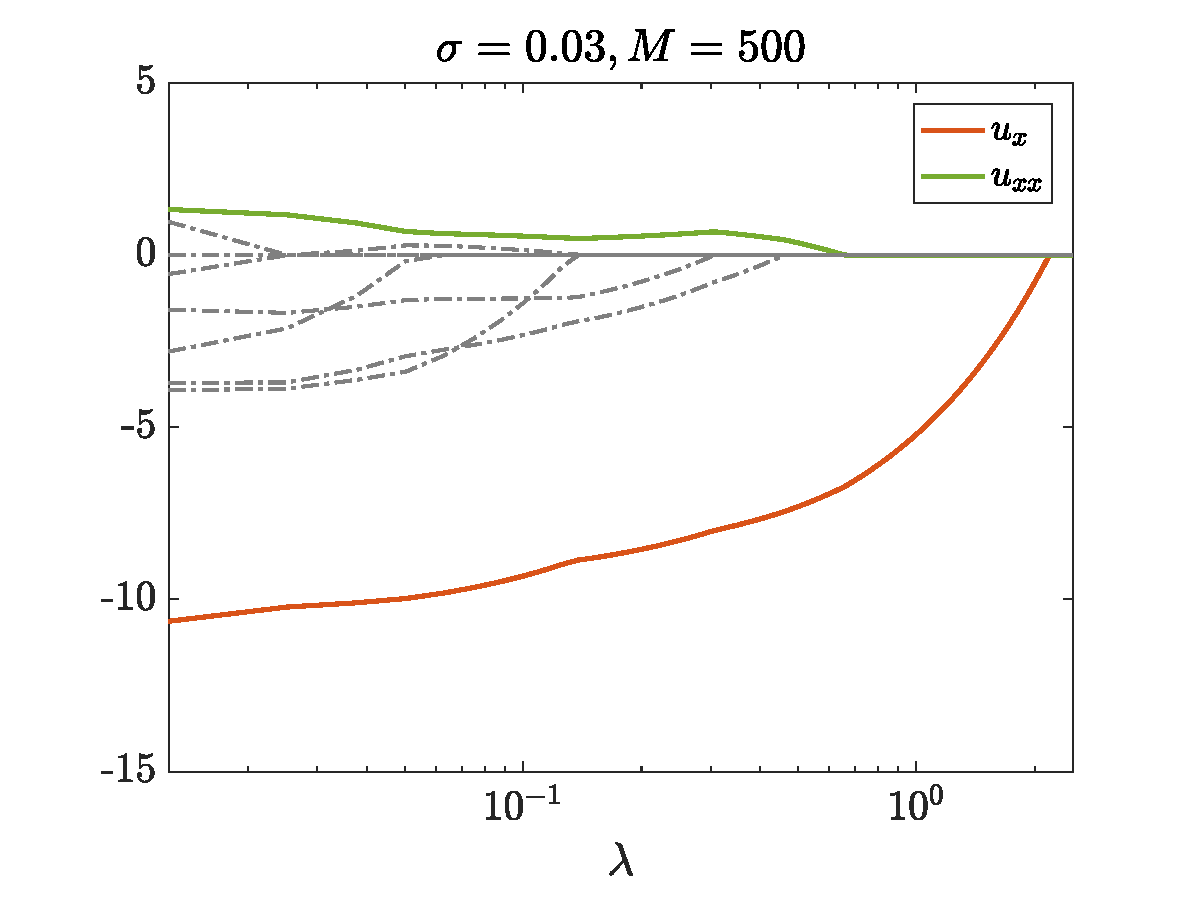
\includegraphics[width=2in]{advdiffExp1_500_0_03.eps}
%\end{tabular}	
%\caption{$\ell_1$-PsL model for PDE identification when the underlying PDE is advection-diffusion equation: $u_t=2u_{xx}-10u_x$ with an observed function: $u(x,t)=\sqrt{0.6/(0.6+8t)}\exp(-(x+0.7-10t)^2/(0.6+8t))$, $0\leq x\leq 3$, $0\leq t\leq 0.5$. (a) $\sigma=0.01, N=50$; (b) $\sigma=0.01, N=100$; (c) $\sigma=0.01, N=500$. (d) $\sigma=0.03, N=50$; (e) $\sigma=0.03, N=100$; (f) $\sigma=0.03, N=500$.}\label{expr.advdiff}
%\end{figure}
%
%
%


\subsection{Mutual Incoherence Condition and Data Size}
The deterministic version of~\eqref{assum2} is commonly employed as an important sufficient condition for exact sparse recovery. In Section~\ref{sec.MIP}, we relate this condition to the exhibition of characteristic behaviors of the underlying PDE, such as advection (in relation to $u_x$) and diffusion (in relation to $u_{xx}$). It is known that justifying the deterministic mutual incoherence property is NP-hard~\cite{tillmann2013computational}, thus validating~\eqref{assum2} for an unknown PDE and an arbitrary set of candidate feature variables is  impractical. Instead, we focus on a  concrete example where~\eqref{assum2} holds with high probability provided as the data size increases.

In particular, we study the transport equation:
\begin{align}
&u_t(x,t) = au_x\;,x\in\mathbb{R},~0<t<T_{\max}\;.\label{eq.adv.PDE}\\
&u(x,0)=f(x)\;, x\in\mathbb{R}\;.\label{eq.adv.ival}
\end{align}
where $a$ represents the advection speed. Notice that, although~\eqref{eq.adv.PDE}--\eqref{eq.adv.ival} specifies the PDE satisfied by $u$ over $\mathbb{R}$, the data $\mathcal{D}$ is only restricted within $0\leq x\leq X_{\max}$.  The solution to~\eqref{eq.adv.PDE}--\eqref{eq.adv.ival} is simply $u(x,t)=f(x+at)$, and our discussion below is based on the choices: $a=-2$, $X_{\max}=1$, $T_{\max}=1$, and $f(x)=2\sin 4x$, so that $u(x,t)=2\sin(4x-8t)$.

Before running the simulation, we slightly modify the implementation for local polynomial regression to largely reduce the computational cost. For the estimations of the values near the boundary, we symmetrically pad the time and space domain to compensate the missing points. This is equivalent to numerically imposing a Neumann boundary condition, i.e., the first-order partial derivatives are $0$. The implementation becomes simpler and the computation is $90\%$ faster.  More advanced techniques for addressing the boundary estimations can be found in~\cite{cheng1997automatic,hastie1993local}.

\begin{figure}
\centering
\begin{tabular}{ccc}
(a)&(b)&(c)\\
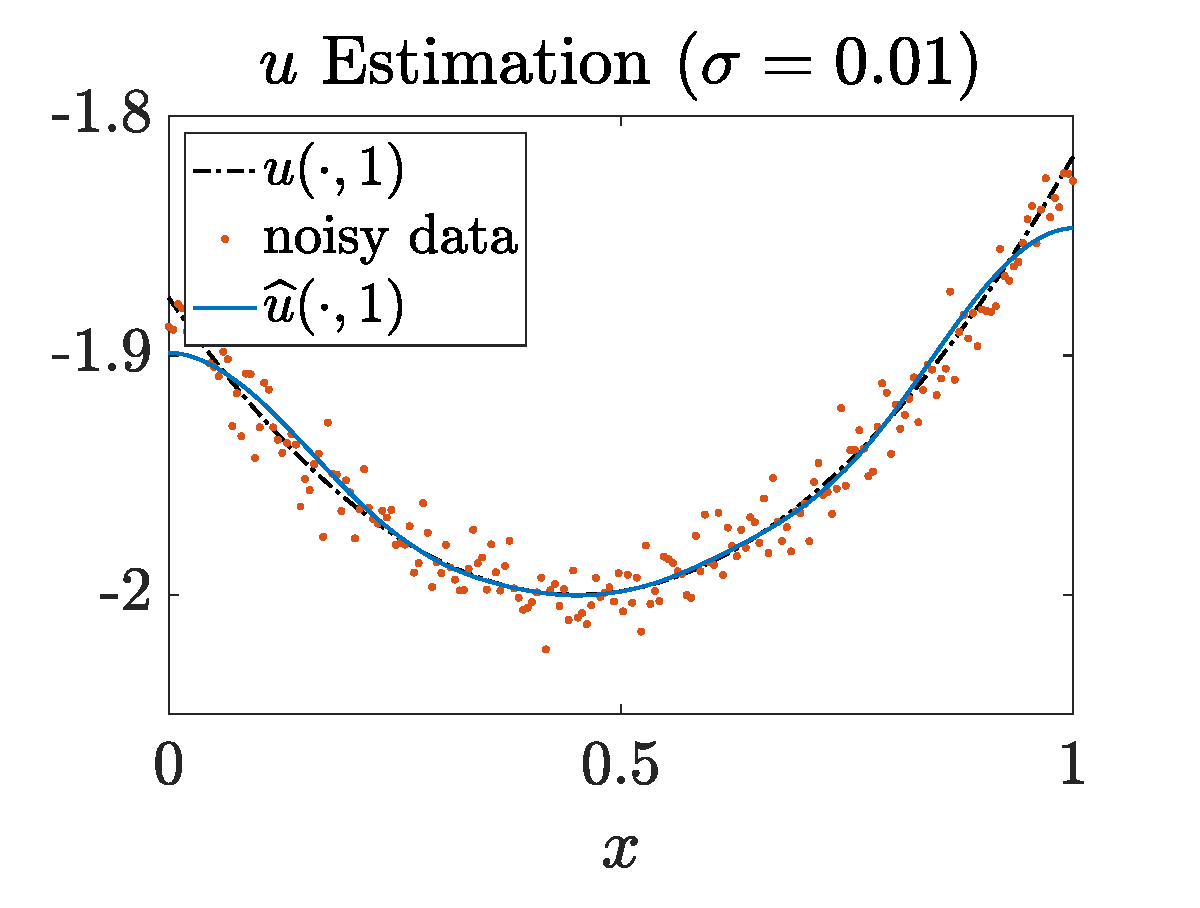
\includegraphics[width=2in]{Figures/localpolyExp1.eps}&
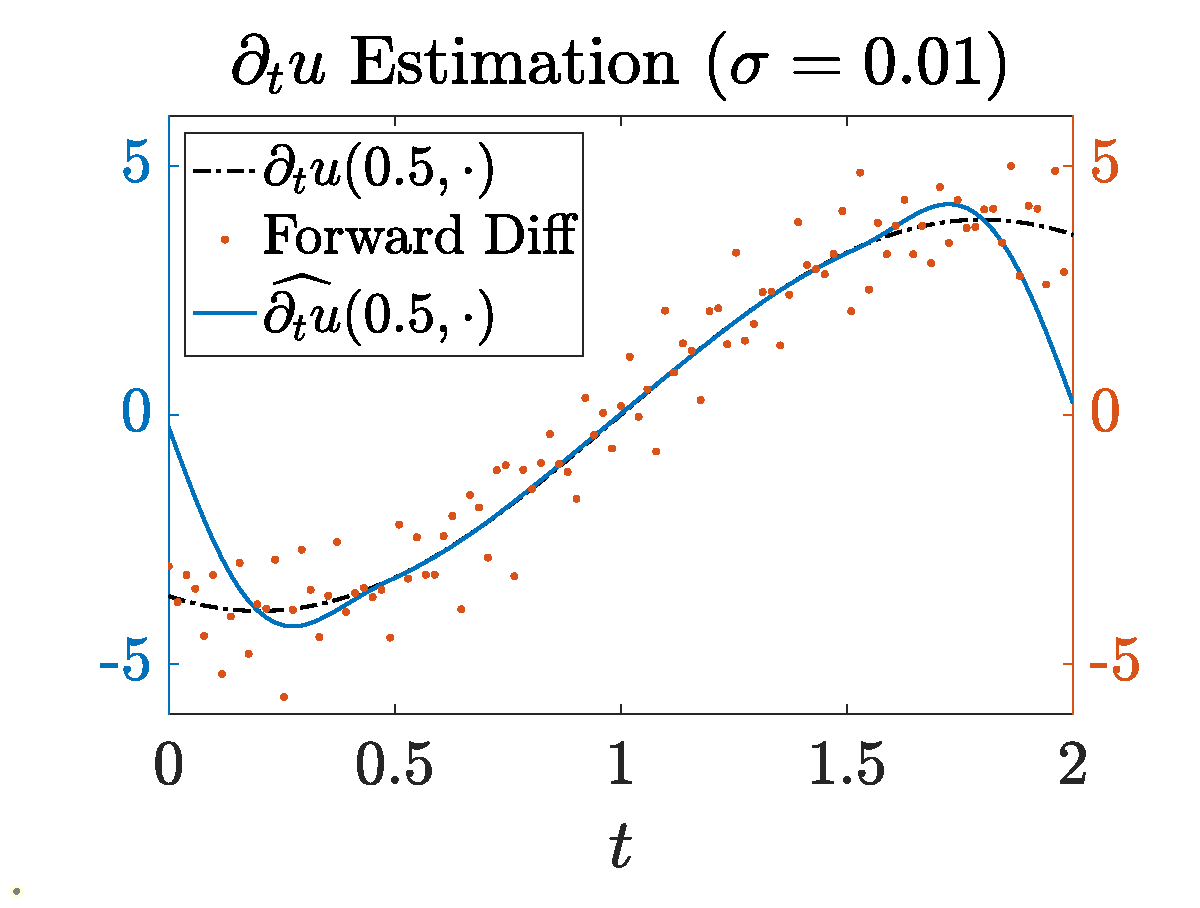
\includegraphics[width=2in]{Figures/localpolyExp3.eps}&
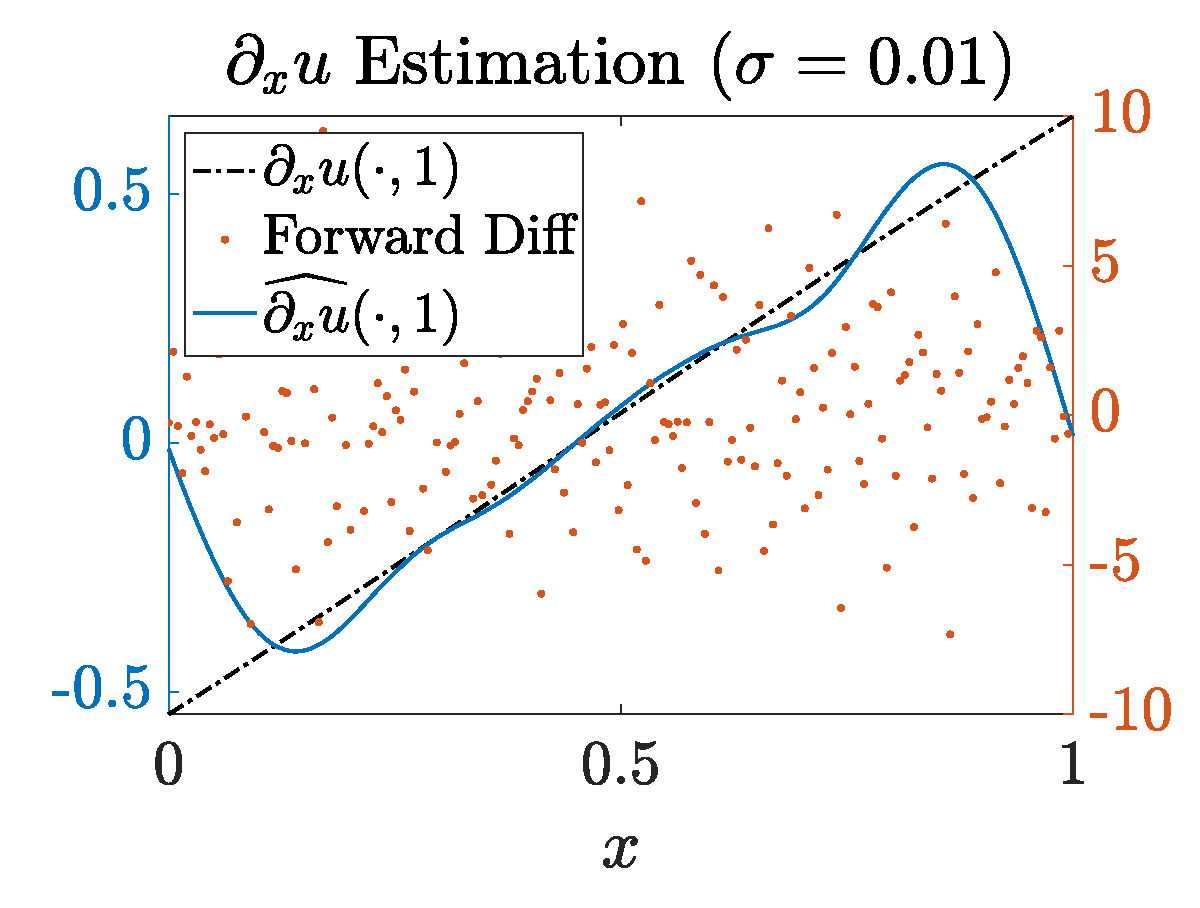
\includegraphics[width=2in]{Figures/localpolyExp2.eps}
\end{tabular}
\caption{Local polynomial regression estimation using symmetric padding for the values near the boundary. Here, the data, data-size, and noise levels are same as those in Figure~\ref{fig.derapprox}; $h_N=N^{-1/7}\approx0.5158$ and $w_M=0.8M^{-1/8}\approx0.4125$. The computation is $90\%$ faster than the one for the estimations in Figure~\ref{fig.derapprox}.}\label{fig.derapprox1}	
\end{figure}



Figure~\ref{fig.MIPtransport} shows the $\ell_\infty$-norm  $||\widehat{\mathbf{F}}_{\mathcal{S}^c}^T\widehat{\mathbf{F}}_{\mathcal{S}}\big(\widehat{\mathbf{F}}_{\mathcal{S}}^T\widehat{\mathbf{F}}_{\mathcal{S}}\big)^{-1}||_\infty$ for noise level $\sigma=0.1$ in (a) and $\sigma=0.3$ in (b) as the data size increases. If this $\ell_\infty$-norm is below $1$, \eqref{assum2} holds. Hence we can see that in both cases, \eqref{assum2} is satisfied with high probability when more data is provided. Notice that when the noise level is high, the number of data required for satisfying  \eqref{assum2} also rises. Moreover,  when the data size is relatively small, adding some noise to the data may lead to  satisfaction of~\eqref{assum2}, even if it does not hold when the data is clean. Different from reducing $||\widehat{\mathbf{F}}_{\mathcal{S}^c}^T\widehat{\mathbf{F}}_{\mathcal{S}}\big(\widehat{\mathbf{F}}_{\mathcal{S}}^T\widehat{\mathbf{F}}_{\mathcal{S}}\big)^{-1}||_\infty$ by  enhancing the resolution, the $\ell_\infty$-norm reduction induced by adding noise is unstable, and the underlying dynamics can be deformed.
\begin{figure}
\centering
\begin{tabular}{c}
(a)\\
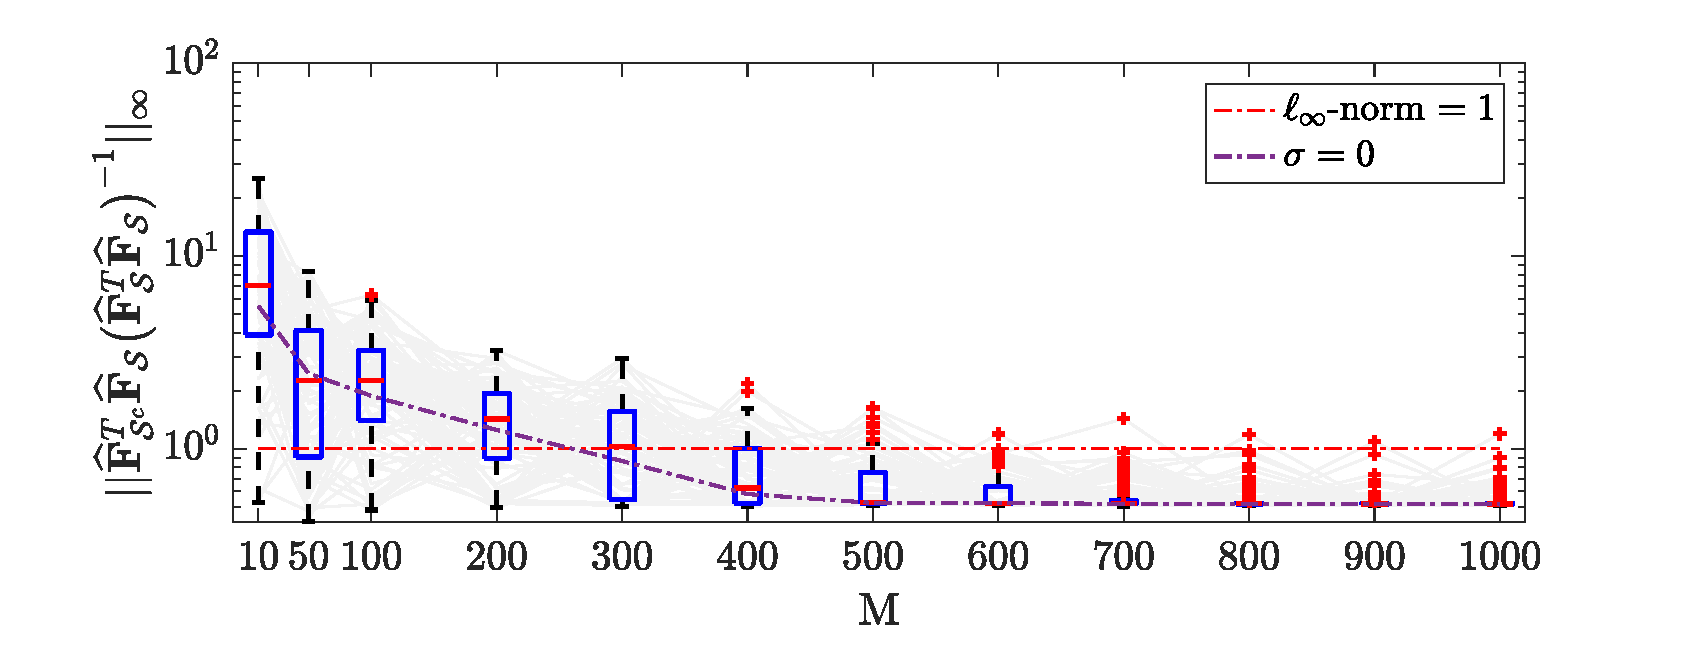
\includegraphics[scale=0.5]{Figures/transportMIP_0_1.eps}\\
(b)\\
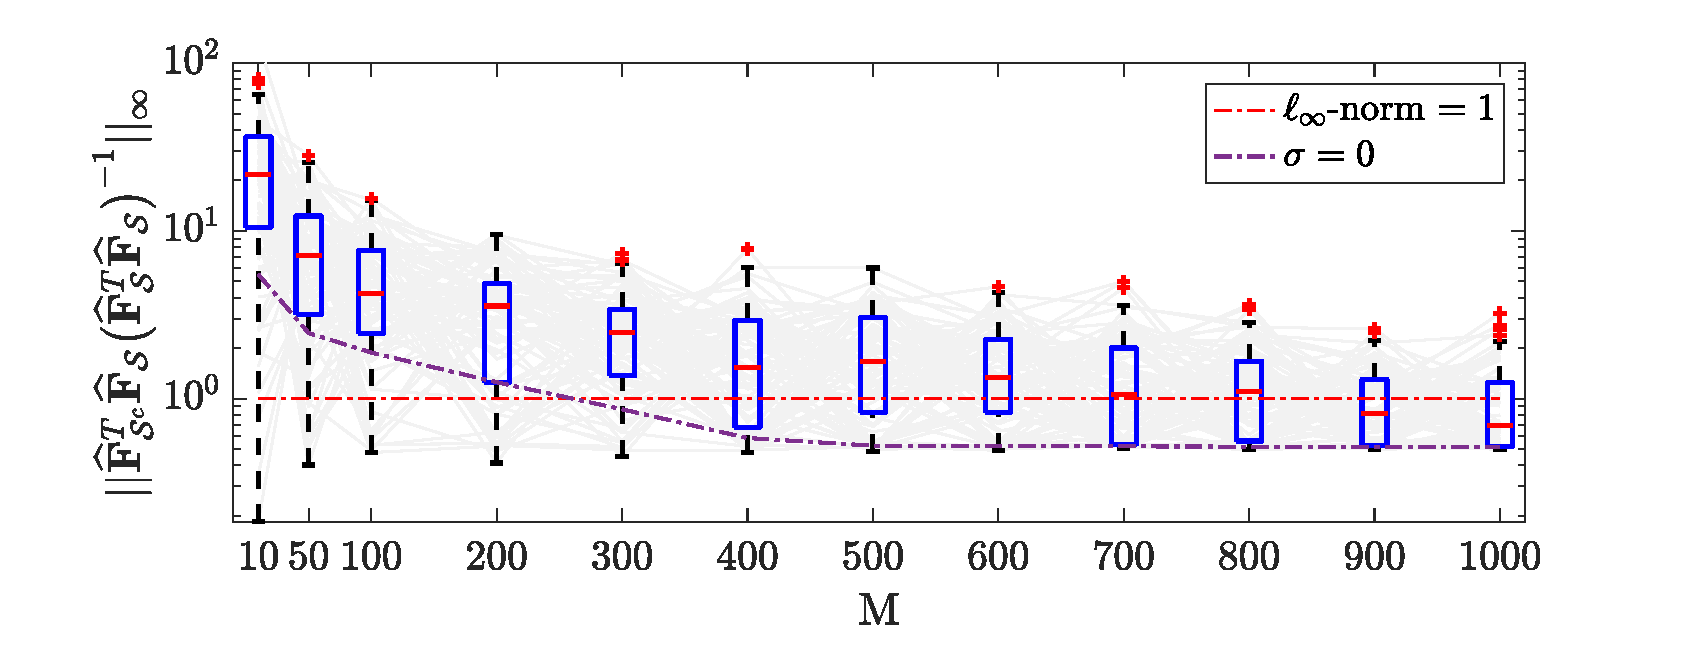
\includegraphics[scale=0.5]{Figures/transportMIP_0_3.eps}
\end{tabular}
\caption{Plot of $||\widehat{\mathbf{F}}_{\mathcal{S}^c}^T\widehat{\mathbf{F}}_{\mathcal{S}}\big(\widehat{\mathbf{F}}_{\mathcal{S}}^T\widehat{\mathbf{F}}_{\mathcal{S}}\big)^{-1}||_\infty$  computed based on the noisy data from $u(x,t)=2\sin(4x-8t)$ satisfying the PDE~\eqref{eq.adv.PDE}--\eqref{eq.adv.ival} with Gaussian noise of intensity (a) $\sigma=0.1$, (b) $\sigma=0.3$. The boxplots are obtained by $100$ independent experiments. As the data size increases ($M=N^{8/7}\to\infty$), this $\ell_\infty$-norm reduces below $1$ on average, indicating that the mutual incoherence condition~\eqref{assum2} holds with high probability with sufficiently many data in this case. }\label{fig.MIPtransport}
\end{figure}



\subsection{Mutual Incoherence Condition and the Observed Solution}
Suppose the underlying PDE is a transport equation $u_t=-(c/\omega)u_x$, $0\leq x\leq X_{\max}$, $0\leq t\leq T_{\max}$ which admits the solutuon: $u(x,t)=A\sin(\omega x-ct)$ for $A\neq 0$. For PDE identification, we choose constant, $u$, $u_x$ and $u_{xx}$ to be the candidate feature variables.

Provided with sufficiently many data, we note that both~\eqref{assum1} and~\eqref{assum3} hold trivially for transport equation, and the deterministic version of~\eqref{assum2}  holds if and only if
\begin{align}
H(\omega,c):=\frac{\max\{\abs{\langle 1,u_x\rangle_{L^2(\Omega)}},\abs{\langle u,u_x\rangle_{L^2(\Omega)}},\abs{\langle u_{xx},u_x\rangle_{L^2(\Omega)}}\}}{||u_x||^2_{L^2(\Omega)}}<1-\mu	\label{MIP.trans}
\end{align}
%If we do not have constant as one of the candidates, the function $H(\omega,c)$ is independent of the magnitude $A$.
Therefore,  in this case, if~\eqref{MIP.trans} holds, all the assumptions in Section~\ref{sec.assumptions} are satisfied; and we can apply Theorem~\ref{thm1} to guarantee recovery of $u_x$ when $\lambda$ is greater than some threshold.

We plot the contour of $H(\omega,c)$ in Figure~\ref{MIPtestExample} (a) when $X_{\max}=T_{\max}=A=0.5$. On the yellow region, $H(\omega,c)>1$, thus~\eqref{assum2} fails; on the light green region,  $0.5<H(\omega,c)<1$, and on the dark green region, $H(\omega,c)<0.5$.  Although~\eqref{assum2} is only a sufficient condition for recovering the feature, in this example, we identify the wrong feature variable $u$ as $\lambda$ increases if the pair $(\omega,c)$ is deeply inside the yellow region ($H(\omega,c)\gg 1$). See (b) and (c). When $(\omega,c)$ resides inside the dark green region ($H(\omega,c)<0.5$), the correct feature $u_x$ is chosen, as shown in (d).


If we vary the domain size $X_{\max}$, the observation time $T_{\max}$, or the magnitude of the the solution $A$, the contour of $H(\omega,c)$ will be modified accordingly. In Figure~\ref{fig.MIPtest1}, we fix $T_{\max}=0.5$ and $A=0.1$; as we increase $T_{\max}$, the yellow region gradually shrinks its area and flattens toward the $c$-axis. In Figure~\ref{fig.MIPtest2}, we fix $X_{\max}=0.5$ and $A=0.1$; as the $X_{\max}$ gets larger, the yellow region also shrinks its area and flattens toward the $\omega$-axis. The effects of increasing the magnitude $A$ are illustrated in Figure~\ref{fig.MIPtest3}, where the yellow region shrinks along the diagonal direction towards the origin.

These shrinking behaviors are expected. When the shape of $u(\cdot,t)$ for any $t$ contains sufficient variations (larger $\omega$), increasing the domain of observation, $X_{\max}$, will introduce more complexities into the data that help to distinguish different feature variables. Therefore, the yellow region shrinks and flattens towards the $c$-axis. Similarly, we can explain why the yellow region shrinks and flattens towards the $\omega$-axis as we increase the observation time $T_{\max}$. Changing the magnitude $A$ magnifies any variations in both space and time, hence the yellow region recedes towards the origin.



\begin{figure}
\centering
\includegraphics[scale=0.222]{Figures/MIPtestExample.eps}
\caption{The assumption \eqref{assum2} has deterministic effects on PDE identification. (a) Contour plot of $H(\omega,c)$ defined in~\eqref{MIP.trans}. On the yellow region, $H(\omega,c)>1$, on the light green region,  $0.5<H(\omega,c)<1$, and on the dark green region, $H(\omega,c)<0.5$. The underlying PDE is a transport equation $u_t=-(c/\omega)u_x$, and $A=X_{\max}=T_{\max}=0.5$. Here, only constant, $u$, $u_x$ and $u_{xx}$ are considered as candidates.  (b) Wrong feature is identified when $\omega=0.01,c=3$.  (c) Wrong feature is identified when $\omega=1\times10^{-4},c=8$. Both points in (b) and (c) belong to the yellow region where \eqref{assum2} fails. (d) Correct feature is identified when $\omega=4,c=8$, which lies in the dark green region where \eqref{assum2} holds. {\color{red} (b)(c)(d) are produced using slow  local polynomial regression. Can we use the slow version for single-run, and fast version for simulation?}}	\label{MIPtestExample}
\end{figure}


%
%\begin{align}
%\underbrace{\frac{\abs{\sin(2\omega X_{\max}-2cT_{\max})-\sin(2\omega X_{\max})+\sin(2cT_{\max})}}{\omega\big(4\omega cX_{\max}T_{\max}+1+\cos(2\omega X_{\max}-2cT_{\max})-\cos(2cT_{\max})-\cos(2cT_{\max})\big)}}_{:=H(\omega,c)}	<1-\mu
%\end{align}
\begin{figure}
\centering
\begin{tabular}{ccc}
(a)&(b)&(c)\\
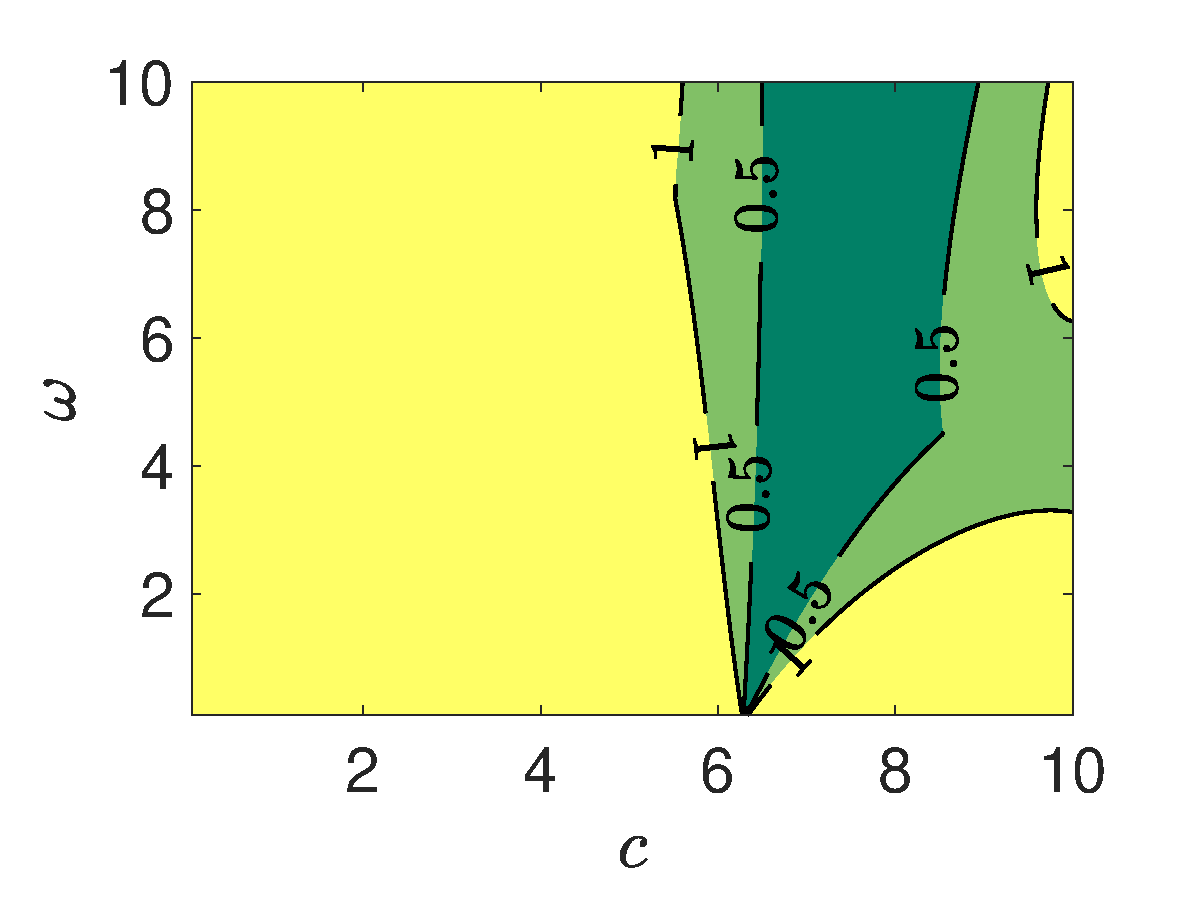
\includegraphics[width=2in]{Figures/MIPcontour1.eps}&
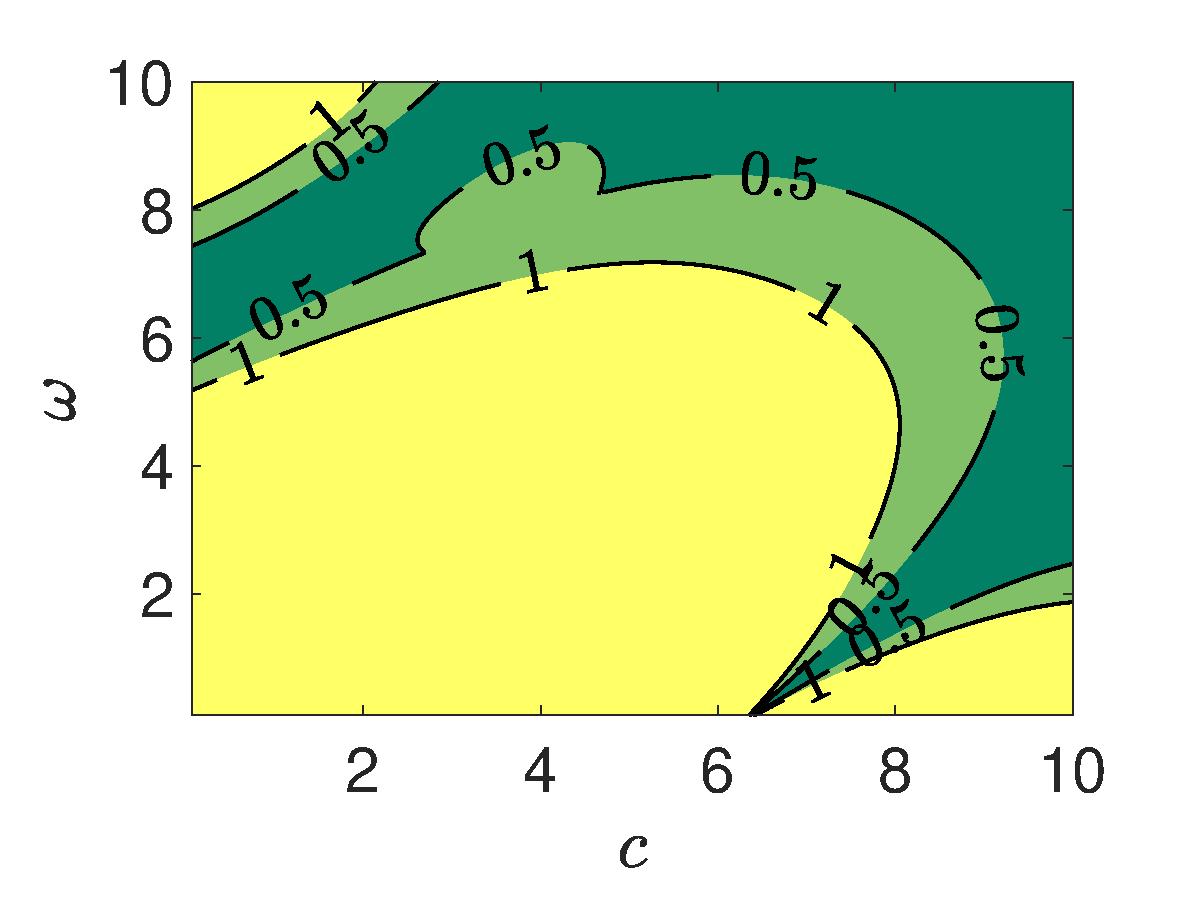
\includegraphics[width=2in]{Figures/MIPcontour2.eps}&
\includegraphics[width=2in]{Figures/MIPcontour3.eps}
\end{tabular}
\caption{Effects of varying domain of observation $X_{\max}$ on the contour of $H(\omega,c)$. (a) $X_{\max}=0.1$; (b) $X_{\max}=0.5$; (c) $X_{\max}=1$.  In all cases, $T_{\max}=0.5$ and $A=0.1$. As $X_{\max}$ increases, the yellow region ($H(\omega,c)>1$) shrinks and flattens towards the $c$-axis.}\label{fig.MIPtest1}
\end{figure}

\begin{figure}
\centering
\begin{tabular}{ccc}
(a)&(b)&(c)\\
\includegraphics[width=2in]{Figures/MIPcontour4.eps}&
\includegraphics[width=2in]{Figures/MIPcontour5.eps}&
\includegraphics[width=2in]{Figures/MIPcontour6.eps}
\end{tabular}
\caption{Effects of varying time of observation $T_{\max}$ on the contour of $H(\omega,c)$. (a) $T_{\max}=0.1$; (b) $T_{\max}=0.4$; (c) $T_{\max}=0.8$.  In all cases, $X_{\max}=0.5$ and $A=0.1$. As $T_{\max}$ increases, the yellow region ($H(\omega,c)>1$) shrinks and flattens towards the $\omega$-axis.}\label{fig.MIPtest2}
\end{figure}


\begin{figure}
\centering
\begin{tabular}{ccc}
(a)&(b)&(c)\\
\includegraphics[width=2in]{Figures/MIPcontour7.eps}&
\includegraphics[width=2in]{Figures/MIPcontour8.eps}&
\includegraphics[width=2in]{Figures/MIPcontour9.eps}
\end{tabular}
\caption{Effects of varying solution magnitude $A$ on the contour of $H(\omega,c)$. (a) $A=0.01$; (b) $A=0.3$; (c) $A=1$.  In all cases, $X_{\max}=0.5$ and $T_{\max}=0.5$. As $A$ increases, the yellow region ($H(\omega,c)>1$) shrinks along the diagonal direction towards the origin.}\label{fig.MIPtest3}
\end{figure}



\subsection{Numerical Validation of Theorem~\ref{thm1}: $\lambda$ Bound}
We numerically demonstrate the implication of Theorem~\ref{thm1}. In particular, we show that the lower bound of the $\ell_1$-regularization parameter $\lambda$ such that $\mathcal{S}(\widehat{\bbeta}^\lambda)\subseteq\mathcal{S}(\bbeta^*)$ holds, behaves as $\sim\sqrt{\ln N/N^{4/7}}$ as the data size $N\to \infty$ (recall that $M=N^{8/7}$). Taking $u(x,t)=2\sin(3x-8t)$ as a solution of the transport equation $u_t=-(8/3)u_x$ and setting $X_{\max}=2$, $T_{\max}=1$,  Figure~\ref{fig.advlambda} shows the lower bound of $\lambda$ that properly recovers the feature variables together with the curve which is some multiple of $\sqrt{\ln N/N^{4/7}}$. The multiple is computed using simple linear regression. The data for (a) is contaminated by Gaussian noise with $\sigma=0.1$ and for (b), the noise level is $\sigma=0.3$. In both cases, the variation of the lower bound for $\lambda$ is well captured by the ratio $\sqrt{\ln N/N^{4/7}}$ as $N\to\infty$. Therefore, Theorem~\ref{thm1} is also numerically validated.
\begin{figure}
\centering
\begin{tabular}{cc}
(a)	& (b)\\
\includegraphics[scale=0.4]{Figures/transport_lambdaexp_0_3.eps}	&
\includegraphics[scale=0.4]{Figures/transport_lambdaexp_1.eps}
\end{tabular}
\caption{As predicted in Theorem~\ref{thm1}, the minimal $\lambda$ required to properly recover $\mS(\bbeta^*)$ decreases in the same order as $\sqrt{\ln N/N^{4/7}}$ when $N\to\infty$. The underlying PDE is $u_t=-(8/3)u_x$, and the data comes from a solution $2\sin(3x-8t)$ with $X_{\max}=2$, $T_{\max}=1$, and noise level $\sigma=0.1$ for (a) and $\sigma=0.3$ for (b). The multipliers in front of $\sqrt{\ln N/N^{4/7}}$ are found via simple linear regression.}\label{fig.advlambda}
\end{figure}


\section{Conclusion}
Formal statistical model selection methods for parameters in PDE models are relatively new in the statistical literature. In this article, we assume that the differential equation models governing the dynamic system are liner PDE. We employ two stage smoothing based method, and apply $\ell_{1}$-PsL for model selection to select correct differential terms. With a properly designed bandwidth parameter, local polynomial regression is used to construct design matrix, and exponential decay rate for achieving strict dual feasibility is obtained, given the constructed design matrix satisfies mutual incoherence property. We provide intuitive insights on how the minimum eigen-value condition and mutual incoherence property can be understood in the PDE context, and how our proposed methods can be applied in identifying two fundamental partial differential equations.

It is noteworthy to mention that the intention of the proposed $\ell_{1}$-PsL method is not to try to improve on the existing methods such as either the cascading method or a Bayesian approach proposed by Xiaolei et al. Though we might loose some estimation efficiency and accuracy, instead we propose our models in the framework of measurement error models to avoid some critical problems of the existing method that includes
1) convergence problem of the Least square methods,
2) high computational cost due to iteratively solving PDE numerically in the estimation proceure; and
3) high computational cost due to complicated optimization problem.

However, there is also a cost associated with the proposed method both from the theoretical and practical points of view. Firstly, a detailed investigation of our proof unveils that the conditions (A2) and (A3) are essential ingredients for obtaining support recovery results in $\ell_{1}$-PsL. Since entries of the estimated feature matrix via local smoothing method are involved with stochasticity, it is desirable to obtain certain probability bounds for the events to happen. However, it turns out that getting the tight bound is a difficult problem, since we don’t know the exact form of the distribution on each entry of gram matrix. Also, as noted by Liang and Wu [], another caveat of our method is that it needs a fair amount of observations for good estimation results for both the response and predictor variables. Particularly, it is a well-known fact that the local kernel smoothing requires a relatively large sample size for the accurate estimates of state variables and their derivatives. A requirement of a large observations for the correct support recovery is also demonstrated by the experiments in Section 4 and 5. We are currently investigating on how to combine our proposed $\ell_{1}$-PsL method with other existing methods to overcome the computational problems of the existing methods, while at the same time put our efforts to see if we can obtain exponentially decaying tail bounds for mutually incoherence quantity for the estimated design matrix, given the ground truth design matrix satisfies mutual incoherence condition. We hope to report some promising results along this line in the near future.

% We employ the local polynomial approximation for the estimators. To simplify the notations, we focus on the case $d=1$. In particular, for an arbitrary point  $X\in\mathbb{R}$ and every $n=1,\cdots,N$, we estimate the partial derivatives with respective to  (wrt.) the spatial dimension by solving the following weighted least square problem:\begin{align}
%\min_{\alpha_j(X,t_n)\in\mathbb{R},j=0,\cdots,p}\sum_{i=1}^{M}(U_i^n-\sum_{j=0}^{p}\alpha_j(X,t_n)(X_i-X)^j)	^2K_w(X_i-X)\;,
%\end{align}
%and setting $\widehat{u^{(j)}(X,t_n)}=j!\alpha_j(X,t_n)$, $j=0,1,\cdots,p$. Here $K_w(\cdot)$ is a symmetric kernel function with bandwidth $w$.  Similarly, with a kernel $K_h$, for arbitrary $t\in\mathbb{R}_+$ and every $i=1,\cdots,M$, we obtain estimators $\widehat{\partial_tu}(X_i,t)$ using local polynomials with degree $q$. Notice that $w$ and $h$ as well as $p$ and $q$ can be different.
%\newpage
\appendix
\section{Proof of Theorem~\ref{thm1}}\label{app.proofthm1}
\subsection{Preparation}
By the KKT-condition, any minimizer $\bbeta$ of~\eqref{eq.lassomat} satisfies:
\begin{align}
-\frac{1}{NM}\widehat{\bF}^T(\widehat{\bu}_t-\widehat{\bF}\bbeta)+\lambda \mathbf{z}=0\;,~\text{for}~\mathbf{z}\in\partial||\bbeta||_1\;,\label{eqKKT}
\end{align}
where $\partial||\bbeta||_1$ denotes the subdifferential of $||\bbeta||_1$. Let $\Delta \bu_t=\widehat{\bu}_t-\bu_t$, $\Delta \bF=\widehat{\bF}-\bF$ denote the error terms, and notice that $\widehat{\bu}_t=\widehat{\bF}\bbeta^*-\Delta \bF\bbeta^*+\Delta \bu_t$, thus from~\eqref{eqKKT}, we get
\begin{align}
&\widehat{\bF}^T\widehat{\bF}(\bbeta-\bbeta^*)+\widehat{\bF}^T(\Delta \bF\bbeta^*-\Delta \bu_t)+\lambda NM\mathbf{z}=0\;~\label{eqKKT2}.
\end{align}
We decompose \eqref{eqKKT2} as follows:
\begin{align}
\begin{bmatrix}
\widehat{\bF}^T_S\widehat{\bF}_\mS&\widehat{\bF}^T_\mS\widehat{\bF}_{\mS^c}\\
\widehat{\bF}^T_{\mS^c}\widehat{\bF}_\mS&\widehat{\bF}^T_{\mS^c}\widehat{\bF}_{\mS^c}
\end{bmatrix}\begin{bmatrix}
\bbeta-\bbeta^*\\
\bbeta_{S^c}
\end{bmatrix}
+\begin{bmatrix}
\widehat{\bF}_\mS^T\\
\widehat{\bF}_{\mS^c}^T
\end{bmatrix}(\Delta \bF_\mS\bbeta_\mS^*-\Delta \bu_t)
+\lambda NM\begin{bmatrix}
\mathbf{z}_\mS\\
\mathbf{z}_{\mS^c}
\end{bmatrix}=\begin{bmatrix}
	\mathbf{0}\\\mathbf{0}
\end{bmatrix}\;.\label{matKKT}
\end{align}
Suppose $(\check{\bbeta},\check{\mathbf{z}})\in\mathbb{R}^K\times\mathbb{R}^K$ is a pair obtained by the primal-dual witness construction, where $\check{\bbeta}_{\mS^c}=0$ and $\check{\mathbf{z}}$ is an element of the subdifferential of $||\check{\bbeta}||_1$.  Plugging $(\check{\bbeta},\check{\mathbf{z}})$ into \eqref{matKKT} gives:
\begin{align}
\check{\mathbf{z}}_{\mS^c}=\widehat{\bF}_{\mS^c}^T\widehat{\bF}_\mS(\widehat{\bF}_{\mS}^T\widehat{\bF}_\mS)^{-1}\mathbf{z}_\mS-\frac{1}{\lambda MN}\widehat{\bF}_{\mS^c}^T{\bf{\Pi}}(\Delta \bF_\mS\bbeta_\mS^*-\Delta \bu_t)\;,\label{zSc}
\end{align}
where ${\bf{\Pi}}={\bf{I}}-\widehat{\bF}_\mS(\widehat{\bF}_\mS^T\widehat{\bF}_S)^{-1}\widehat{\bF}_\mS^T$ is an orthogonal projection. By the complementary slackness condition,  $|\check{\mathbf{z}}_j|< 1$ implies $\check{\bbeta}_j=\mathbf{0}$, which guarantees the proper support recovery. By~\eqref{assum1}, we can focus on proving that, as $N,M\to \infty$, $
\mathbb{P}\big[\max_{j\in \mS^c}|\widetilde{Z}_j|\geq s\big]\to 0$, for $\widetilde{Z}_j = [\widehat{\bF}_{\mS^c}]^T_j{\bf\Pi}\frac{\Delta \bF_\mS\bbeta_\mS^*-\Delta \bu_t}{\lambda NM}$, $[\widehat{\bF}_{\mS^c}]_j$ is the $j$-th column of $\widehat{\bF}_{\mS^c}$. By the following lemma, we claim that to prove Theorem~\ref{thm1}, it suffices to bound $\ell_\infty$-norm of the PDE estimation error $\btau$.
\begin{lemma}\label{Zlemma}
For any $\varepsilon>0$:
\begin{align}
\mathbb{P}\big[\max_{j\in \mS^c}|\widetilde{Z}_j|>\varepsilon\big]\leq  \mathbb{P}\Big[||\btau||_\infty>\frac{\lambda\varepsilon}{\sqrt{K}}\Big]\;.\label{ZlemmaBound}
\end{align}
\end{lemma}
\begin{proof}
	\begin{align*}
	\mathbb{P}\Big[||\widehat{\bF}_{\mS^c}^T{\bf\Pi}\frac{\btau}{\lambda NM}||_\infty>\varepsilon\Big]&\leq\mathbb{P}\Big[||\widehat{\bF}^T{\bf\Pi}\frac{\btau}{\lambda NM}||_2>\varepsilon\Big]\\
	&\leq\mathbb{P}\Big[||\widehat{\bF}||_2\,||\frac{\btau}{\lambda NM}||_2>\varepsilon\Big]\\
	&\leq \mathbb{P}\Big[||\btau||_2>\lambda \varepsilon\sqrt{\frac{NM}{K}}\Big]\leq \mathbb{P}\Big[||\btau||_\infty>\frac{\lambda\varepsilon}{\sqrt{K}}\Big]
	\end{align*}
\end{proof}

\subsection{Sufficient conditions for bounding $\widehat{\bu}_t-\bu_t$}
\begin{prop}\label{prop.Deltat}
For any fixed $i=0,\cdots,M-1$, denote $\eta^2 = \max_{n=0,\cdots,N-1}E(U_i^n)^2$, $\mathcal{K}^*_{\max}=||\mathcal{K}^*||_\infty$. There exist finite positive constants $A(X_i),\overline{C}(X_i),C,L,Q$ which do not depend on the temporal sample size $N$, such that for any $\gamma>0$ and $\varepsilon_N^*$ satisfying:
\begin{align*}
&\varepsilon_N^*(X_i)>\\
&\max\{2|C^*(X_i)|h_N^2,\frac{12\mathcal{K}^*_{\max}B_N}{Nh_N^2},12A(X_i)B_N^{1-s},\frac{12B_N(C\log N+\gamma)\log N}{h_N^2N},12\overline{C}(X_i)\sqrt{\frac{2\ln1/h_N}{h_N^3N}}\}\;,	
\end{align*}
where $B_N$ is an arbitrary increasing sequence $B_N\to\infty$ as $N\to\infty$, we have:
\begin{align}
\mathbb{P}\Big[\sup_{t\in[0,T]}|\Delta u_t(X_i,t)|>\varepsilon_N^*(X_i)\Big]<2N \exp(-\frac{C_N^2}{2\sigma^2})+Qe^{-L\gamma}+4\sqrt{2}\eta^4\exp(-72N)\;,\label{eq.boundDut}
\end{align}
where $C_N =B_N-||u||_{L^\infty(\Omega)}$.
\end{prop}

\begin{proof}
In the following argument, since we have fixed $i=0,\cdots, M-1$, we will omit the dependence of the constants on $X_i$ in the notations. Let $B_N$ be a sequence of increasing positive numbers such that $B_N\to \infty$ as $N\to\infty$, then define the truncated estimate:
\begin{align}
	\widehat{u_t}^B(X_i,t)&=\frac{1}{Nh^2_N}\sum_{n=0}^{N-1}\mathcal{K}^*(\frac{t_n-t}{h_N})U_i^n I\{|U_i^n|<B_N\}\\
	&=\frac{1}{h^2_N}\iint_{|y|<B_N}\mathcal{K}^*(\frac{z-t}{h_N})y\,df_N(z,y)
\end{align}
where $f_N(\cdot,\cdot):=f_N(\cdot,\cdot|X_i)$ is the empirical distribution of $(t_n,U_i^n)$. Construct another increasing sequence by $C_N = B_N-||u||_{L^\infty(\Omega)}$ (which is positive if we take sufficiently large $N$), and notice that for any $\varepsilon\geq \frac{\mathcal{K}^*_{\max}B_N}{Nh_N^2}$:
\begin{align*}
\mathbb{P}\Big[\sup_t|\widehat{u_t}(X_i,t)-\widehat{u_t}^B(X_i,t)|>\varepsilon\Big]&=\mathbb{P}\Big[\sup_t |\frac{1}{Nh^2_N}\sum_{n=0}^{N-1}\mathcal{K}^*(\frac{t_n-t}{h_N})U_i^n I\{|U_i^n|\geq B_N\}|>\varepsilon\Big]\\
&\leq \mathbb{P}\Big[\frac{\mathcal{K}^*_{\max}}{Nh_N^2}\sum_{n=0}^{N-1}|U_i^n|I\{|U_i^n|\geq B_N\}>\varepsilon\Big]\\
&\leq \mathbb{P}\Big[\exists n=0,1,\cdots, N-1,~|U_i^n|\geq B_N\Big]\\
& = \mathbb{P}\Big[\max_{n=0,1,\cdots,N-1}|U_i^n|\geq B_N\Big]\\
&\leq \mathbb{P}\Big[\max_{n=0,1,\cdots, N-1}|U_i^n-u_i^n|\geq C_N\Big]\leq 2N \exp(-\frac{C_N^2}{2\sigma^2})\;.
\end{align*}
On the other hand, from Proposition 1 of~\cite{mack1982weak}:
\begin{align*}
E|\widehat{u_t}(X_i,t)-\widehat{u_t}^B(X_i,t)|\leq AB_N^{1-s}\;.
\end{align*}
for $A=\int|\mathcal{K}(\zeta)|\,d\zeta\times\sup_{t}\int|y|^sf(t,y|X_i)\,dy$ with $f(\cdot,\cdot|X_i)=:f(\cdot,\cdot)$ as the distribution of $(t,U(X_i,t))$; hence for any $\varepsilon_{1,N}\geq \max\{\frac{2\mathcal{K}^*_{\max}B_N}{Nh_N^2},2AB_N^{1-s}\}$, we have:
\begin{align}
&\mathbb{P}\Big[\sup_t|\widehat{u_t}(X_i,t)-\widehat{u_t}^B(X_i,t)-E(\widehat{u_t}(X_i,t)-\widehat{u_t}^B(X_i,t))|>\varepsilon_{1,N}\Big]\leq 2N \exp(-\frac{C_N^2}{2\sigma^2})\;.\label{eq.sup}
\end{align}
Following~\cite{mack1982weak}, we decompose the truncated estimate as follows:
\begin{align*}
\widehat{u_t}^B(X_i,t)=E	\Big[\widehat{u_t}^B(X_i,t)\Big]+\frac{1}{\sqrt{N}}\rho_N(X_i,t)+e_N(X_i,t)\;,
\end{align*}
where
\begin{align}
\rho_N(X_i,t)=\frac{1}{h_N^2}\iint_{|y|<B_N}	\mathcal{K}^*(\frac{t_n-t}{h_N})y\,dB^0(\mathcal{T}(t,y))\;,\label{eq.rhoterm}
\end{align}
with $\mathcal{T}:\mathbb{R}^2\to [0,1]^2$ a distribution transformation defined in~\cite{rosenblatt1952remarks}, and $B^0$ is a sample path of 2D Brownian bridge; and
\begin{align}
e_N(X_i,t)=-\frac{1}{\sqrt{N}h_N^2}\int\Big(\int_{|y|<B_N}y\,d_y\big[Z_N(z,y)-B^0(\mathcal{T}(z,y))\big]\Big)\,d_z \mathcal{K}^*(\frac{z-t}{h_N})\;.	\label{eq.eterm}
\end{align}
with $Z_N(z,y) = \sqrt{N}\big(f_N(z,y)-f(z,y)\big)$ as a 2D-empirical process, where $f(\cdot,\cdot)$ is the distribution function

	$(t_n,U_i^n)$. It is proved in~\cite{tusnady1977remark} that for any $\gamma$:
\begin{align}
\mathbb{P}\Big[\sup_{z,y}|Z_N(t,y)-B^0(\mathcal{T}(z,y))|>\frac{(C\log N+\gamma)\log N}{\sqrt{N}}\Big]<Qe^{-L \gamma}\;,
\end{align}
where $C$, $Q$, and $L$ are absolute positive constants. Therefore, for  $\varepsilon_{2,N}=\frac{2B_N(C\log N+\gamma)\log N}{h_N^2N}$, by change of variable in \eqref{eq.eterm}, we obatin:
\begin{align*}
	\mathbb{P}\Big[\sup_{t}|e_N(X_i,t)|>\varepsilon_{2,N}\Big]&\leq\mathbb{P}\Big[\sup_{t}\frac{2B_N}{h^2_N\sqrt{N}}\sup_{z,y}|Z_N(z,y)-B^0(\mathcal{T}(z,y))|>\varepsilon_{2,N}\Big]<Qe^{-L\gamma}\;.
\end{align*}
As for~\eqref{eq.rhoterm}, similarly to (7) of~\cite{mack1982weak}, we have:
\begin{align*}
\frac{h_N^{3/2}\sup_t|\rho_N(X_i,t)|}{\sqrt{\ln\frac{1}{h_N}}}&\leq 16(\ln V)^{1/2}S^{1/2}\Big(\ln\frac{1}{h_N}\Big)^{-1/2}\int|\zeta|^{1/2}\,|d\mathcal{K}^*(\zeta)|\\
&+16\sqrt{2}h_N^{-1/2}\Big(\ln\frac{1}{h_N}\Big)^{-1/2}\int q(Sh_N|\zeta|)\,|d\mathcal{K}^*(\zeta)|\;,
\end{align*}
%
%\begin{align}
%N^{-1/2}\sqrt{\ln\frac{1}{h_N}}h_N^{-1/2}	
%\end{align}
%
%
%\begin{align*}
%N^{-1/2}\sup_t|\rho_N(X_i,t)|&\leq 16(\ln V)^{1/2}S^{1/2}N^{-1/2}h_N^{-3/2}\int|\zeta|^{1/2}\,|d\mathcal{K}^*(\zeta)|\\
%&+16\sqrt{2}h_N^{-2}N^{-1/2}	\int q(Sh_N|\zeta|)\,|d\mathcal{K}^*(\zeta)|\;,
%\end{align*}
where  $V$ is a random variable satisfying $EV\leq 4\sqrt{2}\eta^4$ for $\eta^2 = \max_{n=0,\cdots,N-1}E(U_i^n)^2$, $q(r)=\int_0^r\frac{1}{2}(\frac{1}{y}\log\frac{1}{y})^{1/2}\,dy$, $S=\sup_t\int y^2f(y,t)\,dy$.  From $\overline{C}=16S^{1/2}\int|\zeta|^{1/2}|d\mathcal{K}^*(\zeta)|$,  for any $\varepsilon_{3,N}>2\overline{C}\sqrt{\frac{2\ln1/h_N}{h_N^3N}}$, then we can bound the probability:
\begin{align}
\mathbb{P}\Big[\sup_t|N^{-1/2}\rho_N(X_i,t)|>\varepsilon_{3,N}\Big]\leq 4\sqrt{2}\eta^4\exp\frac{-N\varepsilon_{3,N}^2h_N^3}{4\overline{C}^2\ln 1/h_N}\;,
\end{align}
when $N$ is large. Combining the results~\eqref{eq.sup}, \eqref{eq.eterm}, and \eqref{eq.rhoterm}, for any
\begin{align*}
\varepsilon_N^*>\max\{2|C^*|h_N^2,\frac{12\mathcal{K}^*_{\max}B_N}{Nh_N^2},12AB_N^{1-s},\frac{12B_N(C\log N+\gamma)\log N}{h_N^2N},12\overline{C}\sqrt{\frac{2\ln1/h_N}{h_N^3N}}\}	\;,
\end{align*}
\begin{align}
\mathbb{P}\Big[\sup_{t\in[0,T]}|\Delta u_t(X_i,t)|>\varepsilon_N^*\Big]<2N \exp(-\frac{C_N^2}{2\sigma^2})+Qe^{-L\gamma}+4\sqrt{2}\eta^4\exp(-72N)\;.
\end{align}
\end{proof}
\begin{remark}
In~\cite{mack1982weak}, there is an additional condition for $B_N$ that, $\sum_{N}B_N^{-s}<\infty$. This is to guarantee that the supremum in~\eqref{eq.sup} is bounded by $B_N^{1-s}$ with probability $1$. In our case, we focus on convergence in probability, hence we do not need this requirement.
\end{remark}
\begin{remark}
From~\cite{fan1997local}, we can obtain the asymptotic bias of this estimator:
\begin{align}
	E\{\widehat{u_t}(X_i,t)\}- u_t(X_i,t)=C^*(X_i)h_N^{2}\;.
\end{align}
for some constant $C^*(X_i)$ that depends on the space point $X_i$. By~\cite{mack1982weak,tusnady1977remark}, under the assumptions stated in Section~\ref{sec.assumptions}, we have:
\begin{align}
\sup_{t\in[0,T]}|\widehat{u_t}(X_i,t)-E\widehat{u_t}(X_i,t)|	=O_P\Big(\sqrt{\frac{-\log h_N}{Nh_N}}\Big)\;.
\end{align}
Therefore, by triangular inequality:
\begin{align}
\sup_{t\in[0,T]}|\Delta u_t(X_i,t)|=	O_P\Big(h_N^2+\sqrt{\frac{-\log h_N}{Nh_N}}\Big)\;.
\end{align}
This expression gives the asymptotic order the error term. Our proof above provides further details of this convergence behavior.
\end{remark}

\subsection{Sufficient conditions for bounding $(\widehat{\bF}-\bF)\bbeta^*$}
%For every fixed $n=0,1,\cdots, N-1$, we employ a one-dimensional local degree $p=1,2,\cdots$ polynomial regression at arbitrary location $x\in [0,X_{\max}]$ by minimizing:
%\begin{align}
%(\widehat{c}^p_j)_{j=0}^p=\arg\min_{c_j(x)\in\mathbb{R},j=0,\cdots,p}\sum_{i=0}^{M-1}\big(u(X_i,t_n)-\sum_{j=0}^{p}c_j(x)(X_i-x)^j\big)^2K\big(\frac{X_i-x}{w_{M,p}}\big)\;,
%\end{align}
%where $w_{M,p}$ is the bandwidth parameter when $p$ is fixed; then we approximate the $p-1$-th order partial derivatives by:
%\begin{align}
%	\widehat{\partial_x^{p}u}(x,t_n):=(p-1)!\,\widehat{c}^p_{p-1}(x),~\forall x\in[0,X_{\max}]\;.
%\end{align}
%For product terms such as $uu_x$, we estimate it using $\widehat{u}\widehat{u}_x$. Notice that, from~\cite{fan1997local}, we can obtain the asymptotic bias of the estimator:
%\begin{align}
%	E\{\widehat{\partial_x^pu}(x,t_n)\}- \partial_x^pu(x,t_n)=C_p^*(t_n)w_M^{2}\;.
%\end{align}
%for some constant $C_p^*(t_n)$ that depends on the time $t_n$ and the order of the derivative $p$.
For the first order partial derivative estimators, we have results similarly to Proposition~\ref{prop.Deltat}.
\begin{prop}\label{prop.Dx}
For any fixed $n=0,\cdots,N-1$, denote $\eta^2 = \max_{n=0,\cdots,N-1}E(U_i^n)^2$, $\mathcal{K}^*_{\max}=||\mathcal{K}^*||_\infty$. There exist finite positive constants $A_p(t_n),\overline{C}_p(t_n),C,L,Q$ which do not depend on the spatial sample size $M$, such that for any $\gamma>0$ and $\varepsilon_M^*$ satisfying:
\begin{align*}
&\varepsilon_{M,p}^*(t_n)>\\
&\max\{2|C_p^*(t_n)|w_{M,p}^2,\frac{12\mathcal{K}^*_{\max}B_M}{Mw_{M,p}^{1+p}},12A_p(t_n)B_M^{1-s},\frac{12B_M(C\log M+\gamma)\log M}{w_{M,p}^{1+p}M},12\overline{C}_p(t_n)\sqrt{\frac{2\ln1/w_M}{w_M^{2+p}M}}\}\;,	
\end{align*}
where $B_M$ is an arbitrary increasing sequence $B_M\to\infty$ as $M\to\infty$, we have:
\begin{align}
\mathbb{P}\Big[\sup_{x\in[0,X_{\max}]}|\widehat{\partial_x^pu}(x,t_n)-\partial_x^pu(x,t_n)|>\varepsilon_{M,p}^*\Big]<2M \exp(-\frac{C_M^2}{2\sigma^2})+Qe^{-L\gamma}+4\sqrt{2}\eta^4\exp(-72M)\;,
\end{align}
where $C_M = B_M-||u||_{L^\infty(\Omega)}$.
\end{prop}
As for the product terms:
\begin{prop}\label{prop.Dxx}
For any fixed $n=0,\cdots,N-1$, denote $\eta^2 = \max_{n=0,\cdots,N-1}E(U_i^n)^2$, $\mathcal{K}^*_{\max}=||\mathcal{K}^*||_\infty$. There exist constants $L$ and $Q$ which do not depend on the spatial sample size $M$, such that for any $\gamma>0$ and $\varepsilon_M^*$ satisfying:
\begin{align*}
\varepsilon_{M,p,q}^*>\max\{3||\partial_x^pu(\cdot,t_n)||_\infty\varepsilon^*_{M,p},~3||\partial_x^qu(\cdot,t_n)||_\infty\varepsilon^*_{M,q},~3(\varepsilon^*_{M,p})^2,~3(\varepsilon^*_{M,q})^2\}
\end{align*}
where $B_M$ is an arbitrary increasing sequence $B_M\to\infty$ as $M\to\infty$; $\varepsilon^*_{M,p}$ and $\varepsilon^*_{M,q}$ are the thresholds in Proposition~\ref{prop.Dx} for the sup-norm bound of the estimator $\widehat{\partial_x^pu}$ and $\widehat{\partial_x^qu}$, respectively, $p,q=0,1,\cdots$, we have:
\begin{align}
&\frac{1}{4}\mathbb{P}\Big[\sup_{x\in[0,X_{\max}]}|\widehat{\partial_x^pu}(x,t_n)\widehat{\partial_x^qu}(x,t_n)-\partial_x^pu(x,t_n)\partial_x^qu(x,t_n)|>\varepsilon_{M,p,q}^*\Big]<\nonumber\\
&2M \exp(-\frac{C_M^2}{2\sigma^2})+Q_{p,q}(t_n)e^{-L_{p,q}(t_n)\gamma}+4\sqrt{2}\eta^4\exp(-72M)\;,
\end{align}	
where $C_M = B_M-||u||_{L^\infty(\Omega)}$.
\end{prop}

\begin{proof}
Notice that for any $\varepsilon>0$, we can bound the probability:
\begin{align*}
&\mathbb{P}\Big[\sup_{x\in[0,X_{\max}]}|\widehat{\partial_x^pu}(x,t_n)\widehat{\partial_x^qu}(x,t_n)-\partial_x^pu(x,t_n)\partial_x^qu(x,t_n)|>\varepsilon\Big]\leq\\
&\leq\mathbb{P}\Big[||\partial_x^pu(\cdot,t_n)||_{\infty}\sup_{x\in[0,X_{\max}]}|\Delta\partial_x^qu(x,t_n)|>\varepsilon/3\Big]+\\
&\mathbb{P}\Big[||\partial_x^qu(\cdot,t_n)||_{\infty}\sup_{x\in[0,X_{\max}]}|\Delta\partial_x^pu(x,t_n)|>\varepsilon/3\Big]+\\
&\mathbb{P}\Big[\sup_{x\in[0,X_{\max}]}|\Delta\partial_x^pu(x,t_n)|>\sqrt{\frac{\varepsilon}{3}}\Big]+\mathbb{P}\Big[\sup_{x\in[0,X_{\max}]}|\Delta\partial_x^qu(x,t_n)|>\sqrt{\frac{\varepsilon}{3}}\Big]\;,
\end{align*}
hence the results follow from Proposition~\ref{prop.Dx}.
\end{proof}
%\subsection{Stochastic truncation error bound}
%Combining the results from Proposition~\ref{prop.Deltat},~\ref{prop.Dx}, and~\ref{prop.Dxx}, we finally reach at the following theorem.
%\begin{thm}~\label{mainThm}
%Denote $\eta^2 = \max_{n=0,\cdots,N-1}E(U_i^n)^2$, $\mathcal{K}^*_{\max}=||\mathcal{K}^*||_\infty$. Using the notations from Proposition~\ref{prop.Deltat},~\ref{prop.Dx}, and~\ref{prop.Dxx}, there exist positive constants $L$ and $Q$, such that for any $\gamma>0$ and $\varepsilon_{N,M}$ satisfying:
%\begin{align*}
%\varepsilon_{N,M}>\max\{(2NK\beta^*_{\max}\varepsilon^*_{M,p})_{p=0,1,\cdots},(2NK\beta^*_{\max}\varepsilon^*_{M,p,q})_{p,q=0,1,\cdots},2M\varepsilon^*_{N}\}	
%\end{align*}
%we have
%\begin{align}
%\mathbb{P}\Big[||\tau||_\infty>\varepsilon_{N,M}\Big]<&4N\Big(1-(1-C_sB_M^{-s})^M+Qe^{-\gamma L}+4\sqrt{2}\eta^4\exp(-72M)\Big)+\nonumber\\
%&M\Big(1-(1-C_sB_N^{-s})^N+Qe^{-\gamma L}+4\sqrt{2}\eta^4\exp(-72N)\Big)\;,
%\end{align}
%where $B_N$ and $B_M$ are arbitrary increasing sequences, $B_N\to\infty$, $B_M\to\infty$ as $N,M\to\infty$, respectively.
%\end{thm}
%\begin{proof}
%The only thing left to check is tha
%
%Notice that
%
%
%\end{proof}

\subsection{Simplification on the Probability Bounds}
We focus on the simplification of~\eqref{eq.boundDut}, and the others follow similarly. Let $a>0$ and $b>0$  be some positive real numbers to be specified, then the bandwidth $h_N$ and the arbitrary increasing $B_N$ take the forms:
\begin{align}
h_N = \frac{1}{N^a},~B_N = N^b\;.	\label{eq.form}
\end{align}
%We require that $h_N<1$, hence a preliminary condition for $a$ and $c$ is that:
%\begin{align}
%\ln\frac{c}{a}<1\;.\label{eq.pre}	
%\end{align}
Note that the threshold $\varepsilon^*_N$ is determined by the maximum of 5 terms, which can be written as follows after plugging the forms in~\eqref{eq.form}:
%\begin{align}
%&E_1(N) = \frac{2|C*(X_i)|\ln^{2c} N}{N^{2a}}\\
%&E_2(N) = \frac{12K_{\max}^*}{N^{1-b-2a}\ln^{2c} N}\\
%&E_3(N) = \frac{12A(X_i)}{N^{b(s-1)}}	\\
%&E_4(N) =\frac{12(C\ln N+\gamma)\ln^{1-2c} N}{N^{1-b-2a}}\label{eq.gamma}\\
%&E_5(N) = 12\overline{C}(X_i)\sqrt{\frac{2a\ln N-2c\ln\ln N}{N^{1-3a}\ln^{3c}N}}\;.
%\end{align}
\begin{align}
&E_1(N) = \frac{2|C^*(X_i)|}{N^{2a}}\\
&E_2(N) = \frac{12K_{\max}^*}{N^{1-b-2a}}\\
&E_3(N) = \frac{12A(X_i)}{N^{b(s-1)}}	\\
&E_4(N) =\frac{12(C\ln N+\gamma)\ln N}{N^{1-b-2a}}\label{eq.gamma}\\
&E_5(N) = 12\overline{C}(X_i)\sqrt{\frac{2a\ln N}{N^{1-3a}}}\;.
\end{align}
In order to have $E_i(N)\to 0$ as $N\to\infty$, it is thus sufficient to have that:
\begin{align}
\begin{cases}
	1-b-2a>0\\
s-1>0\\
	1-3a>0
\end{cases}	
\end{align}
%Considering the preliminary condition~\eqref{eq.pre}, thus need:
%\begin{align}
%	\ln 3c<1\;.
%\end{align}
%Figure~\ref{} shows an illustration of the sufficient region for the pair $(a,b)$.
%\begin{figure}
%\centering
%\begin{tikzpicture}
%      \draw[->] (-3,0) -- (4.2,0) node[right] {$a$};
%      \draw[->] (0,-3) -- (0,4.2) node[above] {$b$};
%      \draw[scale=3,domain=-3/3:4/3,smooth,variable=\x,gray] plot ({1/3},{\x});
%      \draw[scale=3,domain=-3/3:4/3,smooth,variable=\x,gray] plot ({1/15},{\x});
%      \node [text=gray] at (-1.5, 3.4) {$b =-2a + 1$};
%      \node [text=gray] at (2, 3.4) {$a =1/3$};
%      \node [text=gray] at (-1.15, 1.1) {$a = c/\exp(1)$};
%      \draw[scale=3,domain=-2/3:7/3,smooth,variable=\x,gray]  plot ({\x/3},{1-2*\x/3});
%    \end{tikzpicture}	
%\end{figure}


Notice that the probability bound in~\eqref{eq.boundDut} becomes:
\begin{align}
2N \exp(-\frac{(N^b-||u||_{L^\infty(\Omega)})^2}{2\sigma^2})+Qe^{-L\gamma}+4\sqrt{2}\eta^4\exp(-72N)\,,~\label{eq.probbound}
\end{align}
and the free parameter $\gamma$ is related to both probability upper-bound~\eqref{eq.probbound} and the threshold lower-bound~\eqref{eq.gamma}. We take for some $c>0$:
\begin{align}
\gamma = \frac{N^c}{L}\;.
\end{align}
% hence the probability upper-bound \eqref{eq.probbound} is simplified:
%\begin{align}
%2N \exp(-\frac{(N^b-||u||_{L^\infty(\Omega)})^2}{2\sigma^2})+(4\sqrt{2}\eta^4+Q)\exp(-72N)\;,
%\end{align}
%Hence $E_4(N)$ in \eqref{eq.gamma} becomes:
%\begin{align}
%&E_4(N) =\frac{\omega\ln^{2} N}{N^{1-b-2a-r}}	
%\end{align}
%where $\omega = 12(C+\frac{bs-1}{L})$ is a constant independent of $N$.
The optimal choice for such a $c$ satisfies $c\geq \min\{2b,1\}$. When $N$ is sufficiently large, to determine $\varepsilon_N^*$, we only need to focus on comparing the powers of $N$ in $E_i(N)$, $i=1,2,\cdots,6$; this immediately leads to:
\begin{align}
E_2(N)\lesssim E_4(N) \text{~and~} E_3(N)\lesssim E_4(N)	\;,
\end{align}
hence it's sufficient to only consider $E_1(N)$, $E_4(N)$, and $E_5(N)$. The optimal choice of $a$ and $b$ is determined by requiring that $b$ is maximized when the following constraints are satisfied:
\begin{align}
\begin{cases}
	2a = 1-b-2a-c\\
	2a = \frac{1-3a}{2}\\
	c\geq \min\{2b,1\}
\end{cases}	\implies\begin{cases}
a= \frac{1}{7}\\
b = \frac{1}{7}\\
c = \frac{2}{7}	
\end{cases}\label{eq.parchoice}
\end{align}
To summarize the discussion above, we have
\begin{corollary}
For any fixed $i=0,\cdots,M-1$, denote $\eta^2 = \max_{n=0,\cdots,N-1}E(U_i^n)^2$, $\mathcal{K}^*_{\max}=||\mathcal{K}^*||_\infty$. There exist finite constants $C(X_i)$ independent of $N$, such that with sufficiently large $N$ and a bandwidth $h_N = N^{-1/7}$, for any $\varepsilon_N^*(X_i)$ satisfying
\begin{align*}
\varepsilon_N^*(X_i)> \frac{C(X_i)\sqrt{\ln N}}{N^{2/7}}\;,
\end{align*}
we have:
\begin{align}
\mathbb{P}\Big[\sup_{t\in[0,T]}|\Delta u_t(X_i,t)|>\varepsilon_N^*(X_i)\Big]<2N \exp(-\frac{(N^{1/7}-||u||_{L^\infty(\Omega)})^2}{2\sigma^2})\;.\label{eq.SimpleboundDut}
\end{align}
\end{corollary}
\begin{proof}
With the choice of $a,b,c$ in~\eqref{eq.parchoice}, the probability bound~\eqref{eq.probbound} becomes:
\begin{align*}
2N \exp(-\frac{(N^{1/7}-||u||_{L^\infty(\Omega)})^2}{2\sigma^2})+Qe^{-N^{2/7}}+4\sqrt{2}\eta^4\exp(-72N)\sim 2N \exp(-\frac{(N^{1/7}-||u||_{L^\infty(\Omega)})^2}{2\sigma^2})\;.
\end{align*}
Taking $C(X_i) = \max\{2|C^*(X_i)|,12,\sqrt{\frac{288}{7}}\overline{C}(X_i)\}$	and omitting the second order term $(\ln N/N^{2/7})^2$ gives the result.
\end{proof}
Using similar strategy, we can derive analogous results for the spatial derivative errors.
\begin{corollary}\label{cor.singlespace}
For any nonnegative integer $p=0,1,2,\cdots$ and any fixed $n=0,\cdots,N-1$, denote $\eta^2 = \max_{n=0,\cdots,N-1}E(U_i^n)^2$, $\mathcal{K}^*_{\max}=||\mathcal{K}^*||_\infty$. There exist finite constants $C_{p}(t_n)>0$ independent of $M$, such that with sufficiently large $M$ and a bandwidth $w_{M,p} = M^{-1/(6+p)}$, for any $\varepsilon_{M,p}^*$ satisfying:
\begin{align*}
\varepsilon_{M,p}^*(t_n)> \frac{C_{p}(t_n)\sqrt{\ln M}}{M^{2/(6+p)}}\;,
\end{align*}
we have:
\begin{align}
\mathbb{P}\Big[\sup_{x\in[0,X_{\max}]}|\widehat{\partial_x^pu}(x,t_n)-\partial_x^pu(x,t_n)|>\varepsilon_{M,p}^*\Big]<2M \exp(-\frac{(M^{1/(6+p)}-||u||_{L^\infty(\Omega)})^2}{2\sigma^2})
\end{align}	
\end{corollary}


\begin{corollary}\label{cor.doublespace}
For any nonnegative integers $p,q=0,1,2,\cdots$ and any fixed $n=0,\cdots,N-1$, denote $\eta^2 = \max_{n=0,\cdots,N-1}E(U_i^n)^2$, $\mathcal{K}^*_{\max}=||\mathcal{K}^*||_\infty$. There exist finite constants $C_{p,q}(t_n)>0$ independent of $M$, such that with sufficiently large $M$ and a bandwidth $w_{M,p,q} =M^{-1/(6+\max(p,q))}$,  for any $\varepsilon_{M,p,q}^*$ satisfying:
\begin{align*}
\varepsilon_{M,p,q}^*> C_{p,q}(t_n)M^{-2/(6+\max(p,q))}
\end{align*}
we have:
\begin{align}
&\frac{1}{4}\mathbb{P}\Big[\sup_{x\in[0,X_{\max}]}|\widehat{\partial_x^pu}(x,t_n)\widehat{\partial_x^qu}(x,t_n)-\partial_x^pu(x,t_n)\partial_x^qu(x,t_n)|>\varepsilon_{M,p,q}^*\Big]\nonumber\\
&<2M \exp(-\frac{(M^{1/(6+\max\{p,q\})}-||u||_{L^\infty(\Omega)})^2}{2\sigma^2})\;.
\end{align}	
\end{corollary}
\subsection{$\ell_\infty$ Bound for the PDE Estimation Error}
Notice that in the previous results, the constants $C(X_i)$ (independent of $N$), $C_p(t_n)$, $C_{p,q}(t_n)$ (independent of $M$) for the lower bound of the error thresholds depend on the spatial or temporal grid points. To guarantee that as both $N,M\to\infty$, these constants are uniformly bounded, we prove the following lemma.
\begin{lemma}\label{lemma}
For any integer $M\geq 1$, and any $i=0,1,\cdots, M-1$,  $|C^*(X_i)|$ and $\overline{C}(X_i)$ in Corollary~\ref{prop.Deltat} are bounded by constants that are independent of $M$. That is, there exist constants $C^*, \overline{C}(\sigma,||u||_{L^\infty(\Omega)})>0$ such that for any $M\geq 1$
\begin{align}
\max_{i=0,\cdots, M-1}|C^*(X_i)|\leq C^*||\partial_t^3u||_\infty,~\max_{i=0,\cdots, M-1}\overline{C}(X_i)\leq \overline{C}(\sigma,||u||_{L^\infty(\Omega)})\;.
\end{align}
\end{lemma}
\begin{proof}
From (3.7) in the Theorem 3.1 of~\cite{fan1997local}, we see that
\begin{align*}
|C^*(X_i)|\leq C^*||\partial_t^3u||_\infty<\infty
\end{align*}
where $C^*$ only depends on the choice of the kernel function and the order of the local polynomial. For a general $s$, we know that
\begin{align*}
&\sup_{t\in [0,T]}\int |y|^sf(t,y|X_i)\,dy=\sup_{t\in [0,T]}\int |y|^s\frac{1}{\sqrt{2\pi\sigma^2}}\exp(-\frac{(y-u(X_i,t))^2}{2\sigma^2})\,dy\\
&=\sup_{t\in[0,T]}\sigma^s2^{s/2}\frac{\Gamma\big(\frac{1+s}{2}\big)}{\sqrt{\pi}}{_1F_1}(-\frac{s}{2},\frac{1}{2},-\frac{1}{2}\Big(\frac{u(X_i,t)}{\sigma}\Big)^2)
\end{align*}
where ${_1F_1}(a,b,z)$ is Kummer's confluent hypergeometric function of $z\in\mathbb{C}$ with parameters $a,b\in\mathbb{C}$~(See, e.g.\cite{winkelbauer2012moments}). Since ${_1F_1}(-\frac{s}{2},\frac{1}{2},\cdot)$ is an entire function for fixed parameters,
\begin{align*}
\sup_{t\in [0,T]}\int |y|^sf(t,y|X_i)\,dy\leq 	\sup_{t\in[0,T]}\sigma^s2^{s/2}\frac{\Gamma\big(\frac{1+s}{2}\big)}{\sqrt{\pi}}\sup_{z\in [-\frac{\max_{x\in\Omega} u^2(x,t)}{2\sigma^2},-\frac{\min_{x\in\Omega} u^2(x,t)}{2\sigma^2}]}{_1F_1}(-\frac{s}{2},\frac{1}{2},z)<\infty
\end{align*}
which clearly does not depend on $M$. Take $s=2$, we can obtain that $\overline{C}(X_i)\leq \overline{C}(\sigma,||u||_{L^\infty(\Omega)})$ for some $\overline{C}(\sigma,||u||_{L^\infty(\Omega)})$ that only depends on $||u||_{L^\infty(\Omega)}$ and $\sigma$.
\end{proof}
Note that the same proof can derive that the constants in Proposition~\ref{prop.Dx} are also bounded by $N$-independent constants. This technical lemma allows us to state our main theorem:
\begin{thm}\label{theorem.main1}
Denote $\eta^2 = \max_{n=0,\cdots,N-1}E(U_i^n)^2$, $\mathcal{K}^*_{\max}=||\mathcal{K}^*||_\infty$. Suppose the maximal order of spatial partial derivative we consider is $P_{\max} >0$. There exist some constant $C'=C'(||u||_{W^{P_{\max},\infty}},s,\sigma, ||\beta||_\infty,K)$ independent of $N$ and $M$,  such that with sufficiently large $N$ and $M$, using bandwidths $h_N=N^{-1/7}$ in the time direction and $w_{M} = M^{-1/(6+P_{\max})}$ in the space direction, for any $\varepsilon_{N,M}$ satisfying:
\begin{align*}
\varepsilon_{N,M}>C'\max\{\frac{\sqrt{\ln M}}{M^{2/(6+P_{\max})}},\frac{\sqrt{\ln N}}{N^{2/7}}\}	
\end{align*}
we have
%\begin{align}
%\mathbb{P}\Big[||\tau||_\infty>\varepsilon_{N,M}\Big]<&4N \Big(C''_sM^{1-\frac{3s}{6+P_{\max}}}+4\sqrt{2}\eta^4\exp(-72M)\Big)+M\Big(C''_sN^{1-\frac{3s}{7}}+4\sqrt{2}\eta^4\exp(-72N)\Big)\;.\label{ineq.main}
%\end{align}
\begin{align}
\mathbb{P}\Big[||\btau||_\infty>\varepsilon_{N,M}\Big]<&8MNK \exp(-\frac{(M^{1/(6+P_{\max})}-||u||_{L^\infty(\Omega)})^2}{2\sigma^2})+2MN \exp(-\frac{(N^{1/7}-||u||_{L^\infty(\Omega)})^2}{2\sigma^2})\;.\label{ineq.main}
\end{align}
Here $||u||_{W^{P_{\max},\infty}(\Omega)}$ denotes the Sobolev $P_{\max},\infty$-norm of $u$, $s$ the data regularity parameter in Section~\ref{sec.assumptions}, $\sigma$ the noise level, $||\bbeta^*||_\infty$ the maximal absolute coefficient, and $K$ the number of feature variables.

%In particular, setting $M = N^{(6+P_{\max})/7}$ gives:
%\begin{align}
%\mathbb{P}\Big[||\tau||_\infty>\varepsilon_{N,M}\Big]<&(8K+2)N^{(13+P_{\max})/7}\exp(-\frac{(N^{1/7}-||u||_{L^\infty(\Omega)})^2}{2\sigma^2})\;.\label{ineq.main}
%\end{align}

\end{thm}
\begin{proof}
By triangle inequality:
\begin{align*}
||\btau||_\infty&\leq ||\Delta \bF\bbeta^*||_\infty+||\Delta \bu_t||_\infty\;.
\end{align*}
Since
\begin{align*}
||\Delta \bu_t||_\infty\leq \max_{i=0,1,\cdots,M-1}\sup_{t\in[0,T]}|\Delta u_t(X_i,t)|\;,
\end{align*}
then for sufficiently large $N$, we have that if $\frac{\varepsilon_{N,M}}{2}>C_{1}'\ln N/N^{2/7}$ for some constant $C_1'$:
\begin{align*}
\mathbb{P}\Big[||\Delta \bu_t||_\infty>\frac{\varepsilon_{N,M}}{2}\Big]&\leq\mathbb{P}\Big[\max_{i=0,1,\cdots,M-1}\sup_{t\in[0,T]}|\Delta u_t(X_i,t)|>\frac{\varepsilon_{N,M}}{2}\Big]	\\
&\leq \sum_{i=0}^{M-1}\mathbb{P}\Big[\sup_{t\in[0,T]}|\Delta u_t(X_i,t)|>\frac{\varepsilon_{N,M}}{2}\Big]\\
&\leq 2MN \exp(-\frac{(N^{1/7}-||u||_{L^\infty(\Omega)})^2}{2\sigma^2})\;.
\end{align*}
On the other hand, if we denote $\Delta F_k(x,t)$ as the approximation error of the $k$-th feature variable at time $t$ and space $x$, we have
\begin{align*}
||\Delta \bF\bbeta^*||_\infty\leq \max_{n=0,1,\cdots, N}||\beta||_\infty	\sup_{x\in[0,X_{\max}]}\sum_{k=1}^K|\Delta F_{k}(x,t_n)|\;.
\end{align*}
Hence, for sufficiently large $M$ and if $\frac{\varepsilon_{N,M}}{2K||\bbeta^*||_\infty}>C'_2\ln M/M^{2/(6+P_{max})}$ for some constant $C_2'$:
\begin{align*}
\mathbb{P}\Big[||\Delta \bF\bbeta^*||_\infty>\frac{\varepsilon_{N,M}}{2}\Big]&\leq \sum_{n=0}^{N-1}\sum_{k=1}^{K}\mathbb{P}\Big[\sup_{x\in[0,X_{\max}]}|\Delta F_{k}(x,t_n)|>\frac{\varepsilon_{N,M}}{2K||\bbeta^*||_\infty}\Big]\\
&\leq 8NMK \exp(-\frac{(M^{1/(6+\max\{p,q\})}-||u||_{L^\infty(\Omega)})^2}{2\sigma^2})\;.
\end{align*}
Taking $C'=\max\{2C_1',2K||\bbeta^*||_\infty C_2'\}$   proves the theorem.
\end{proof}
\subsection{Final Step of the Proof}
Combining Lemma~\ref{Zlemma} with Theorem~\ref{theorem.main1}, we see that, for any $\varepsilon$, if it satisfies:
\begin{align}
\lambda\varepsilon>C'\sqrt{K}\max\{\frac{\sqrt{\ln M}}{M^{2/(6+P_{\max})}},\frac{\sqrt{\ln N}}{N^{2/7}}\}
\end{align}
then~\eqref{ZlemmaBound} implies
\begin{align}
\mathbb{P}\Big[\max_{j\in \mS^c}|\widetilde{Z}_j|>\varepsilon\Big]\leq 8MNK \exp(-\frac{(M^{1/(6+P_{\max})}-||u||_{L^\infty(\Omega)})^2}{2\sigma^2})+2MN \exp(-\frac{(N^{1/7}-||u||_{L^\infty(\Omega)})^2}{2\sigma^2})\;.
\end{align}
Therefore, if we take $\varepsilon= \mu$, then the following inequality
\begin{align}
\mathbb{P}\Big[||\check{\mathbf{z}}_{\mS^c}||_\infty	\geq1\Big]&\leq \mathbb{P}\Big[||\widehat{\bF}_{\mS^c}^T\widehat{\bF}_\mS(\widehat{\bF}_{\mS}^T\widehat{\bF}_\mS)^{-1}||_\infty\geq 1-\mu\Big]+\mathbb{P}\Big[\max_{j\in \mS^c}|\widetilde{Z}_j|>\mu\Big]
\end{align}
finishes the proof of Theorem~\ref{thm1}.
\section{Proof of Lemma~\ref{nonoise_lemma}}\label{proof_nonoise_lemma}
\begin{proof}
For any grid point $(x_i,t_n)$ on $\Omega=[0,X_{\max}]\times[0,T_{\max}]$, $i=0,1,\cdots,M-1$, $n=0,1,\cdots,N-1$, if $0<x_i<X_{\max}$ and $0<t_n<T_{\max}$, it is called an inner grid point; otherwise, a boundary grid point. Now denote $L$ as the number of rectangles centering at the inner grid points in $\Omega$ with width $\Delta x$, height $\Delta t$; and $L'$ as that of the boundary grid points. We decompose:
\begin{align*}
\int_\Omega \partial_x^ku(x,t)\,dx\,dt&=\underbrace{\sum_{l=1,2,\cdots,L}\int_{\Omega_l}\partial_x^ku(x,t)\,dx\,dt}_{I}+\underbrace{\sum_{l'=1,2,\cdots,L'}\int_{\Omega_{l'}}\partial_x^ku(x,t)\,dx\,dt}_{I'}\;.
\end{align*}
For the first integral, by triangle inequality and Taylor's theorem:
\begin{align*}
&|I-\sum_{l=1,2,\cdots,L}\int_{\Omega_l}\partial_x^ku(x_l,t_l)\,dx\,dt|\\&\leq\sum_{l=1,2,\cdots,L}\int_{\Omega_l}|\partial_x^{k+1}u(\zeta_l,\eta_l)(x-\zeta_l)|\,dx\,dt+\sum_{l=1,2,\cdots,L}\int_{\Omega_l}|\partial_x^k\partial_tu(x_l,t_l)(t-\eta_l)|\,dx\,dt\\
&\leq ||\partial_x^{k+1}u||_{L^\infty(\Omega)}L\Delta x^2\Delta t+||\partial_x^{k}\partial_tu||_{L^\infty(\Omega)}L\Delta t^2\Delta x\;.
\end{align*}
Here $(\zeta_l,\eta_l)$ denote some point in the domain $(x_l-\Delta x/2,x_l+\Delta x/2)\times (t_l-\Delta t/2,t_l+\Delta t/2)$, $l=1,2,\cdots,L$. Similarly, for the second integral, we obtain:
\begin{align*}
|I'-\sum_{l'=1,2,\cdots,L'}\int_{\Omega_{l'}}\partial_x^ku(x_{l'},t_{l'})\,dx\,dt|\leq \frac{1}{2}(||\partial_x^{k+1}u||_{L^\infty(\Omega)}L'\Delta x^2\Delta t+||\partial_x^{k}\partial_tu||_{L^\infty(\Omega)}L'\Delta t^2\Delta x)	\;.
\end{align*}
Note that $L=(M-1)(N-1)$ and $L'=2M+2N-4$, hence
\begin{align*}
&|\int_\Omega\partial_x^ku(x,t)\,dx\,dt-\mathbf{1}^TF_k\Delta x\Delta t|\\
&\leq ||\partial_x^{k+1}u||_{L^\infty(\Omega)}|\Omega|\Delta x+||\partial_x^{k}\partial_tu||_{L^\infty(\Omega)}|\Omega|\Delta t+\frac{1}{2}(||\partial_x^{k+1}u||_{L^\infty(\Omega)}(2X_{\max}\Delta x\Delta t+2T_{\max}\Delta x^2 )+\\
&||\partial_x^{k}\partial_tu||_{L^\infty(\Omega)}(2X_{\max}\Delta t^2+2T_{\max}\Delta x\Delta t))\\
&=o(\Delta x)+o(\Delta t)\,,\text{as~}N,M\to\infty\;.
\end{align*}
The statement for the product feature is similarly proved once we note the following inequality:
\begin{align*}
&|\sum_{l=1,2,\cdots,L}\int_{\Omega_l}\partial_x^ku(x,t)\partial_x^ju(x,t)\,dx\,dt-\sum_{l=1,2,\cdots,L}\int_{\Omega_l}\partial_x^ku(x_l,t_l)\partial_x^ju(x_l,t_l)\,dx\,dt|\\
&\leq\sum_{l=1,2,\cdots,L}\int_{\Omega_l}|\partial_x^ku(x,t)-\partial_x^ku(x_l,t_l)|\,|\partial_x^ju(x,t)|\,dx\,dt+\\
&\sum_{l=1,2,\cdots,L}\int_{\Omega_l}|\partial_x^ku(x_l,t_l)|\,|\partial_x^ju(x,t)-\partial_x^ju(x_l,t_l)|\,dx\,dt\;.
\end{align*}
\end{proof}

\bibliographystyle{unsrt}
\bibliography{references.bib}
\end{document}
